%!TEX root = ../thesis.tex

\chapter{Literature review}
% \section{Introduction}
\paragraph{}
Creation of mesh in FEM can be expensive in terms of time and human resource.
One possible solution is trying to replace the geometric modelling tool in FEM by something more CAD-like.
NURBS, for example, is a standard mathematical model utilized in CAD industry.
Exact CAD geometric boundaries are achieved with the help of the NURBS curve.
This idea to be geometrically exact with a minimum discretization is adopted in Isogeometric analysis developed in 2005 \cite{Hug2005b} and further refined recently \cite{Zhang2007,Hug2005b,Cot2006,Cot2009,Baz2006a,Baz2006b}.
Furthermore, a simplified mesh refinement method by omitting the necessity for communication with the CAD geometry once the initial shape is received is also targeted \cite{Cot2007}.
% It shows advantage in the structure analysis (fig.~\ref{thinshell}) , fluid mechanics \citep{Buf2011} and dynamics (fig.~\ref{Femvsnurbs}).
The objectives of Isogeometric Analysis are to generalize the meshing process and improve the conventional Finite Element Analysis in the following ways \cite{Aur2010}.
\begin{enumerate}
    \item Offering remarkable degree of accuracy in representing complicated conformations and describing ordinary engineering moulds especially conic sections exactly.
    \item Minimizing geometrical errors and maintain high degree of accuracy in description of geometry at coarsest level of discretization
    \item Simplifying mesh refinement radically by omitting the necessity for communication with the CAD geometry
\end{enumerate}

\paragraph{}
Tensor product Non-Uniform Rational B-spline (NURBS) are well-known curve and surface representation method and have been adopted as a standard in computer graphics, computer-aided-design (CAD) \cite{Nas2003} and Initial Graphics Exchange Specification (IGES) standard since 1983 \cite{IGES1983}.
Nowadays, The employment of rational polynomial functions in description of geometry in CAD/CAM applications is becoming more and more extensive \cite{Pie1987}.
A general sculptured surface can be built easily with the help of NURBS \cite{Rog2001}.
One of its strongest reasons for that is its ability to represent conic curves and surface precisely.

\paragraph{}
The reason why the geometry is represented differently in computer aided design (CAD) and finite element analysis is because of different time they were born.
Commercial software with FEM has already been designed by the late 1960s and it spread to other engineering fields due to its convenience and accuracy.
It employs variational methods (the Calculus of variations) to minimize the error function in order to achieve a converge solution.
However, CAD, which gives an exact description on geometry, has not been developed until 1980s \cite{Dav2008}.
The first uni-graphics System (for 2D modelling and drafting) was sold by United Computing in 1975 \cite{Ste2010}.
Nowadays, CAD has been widespread and wins even more popularity than finite element analysis does. While, the geometric descriptions adopted by engineers today for CAD and analysis are totally different.
One rough estimate \cite{Hug2005} suggests that more than half of the overall analysis time is spent on meshing in the industries such as automotive and aerospace where complex shapes are involved.
Furthermore, frequent design modifications in fast pace, modern society restricts the usage of analysis if a new mesh cannot be created in a short duration.

\paragraph{}
In current Isogeometric analysis, accuracy problems with numerical integration of a rational polynomials attract significant attention \cite{Hug2010,Sev2011,Aur2012}.
Furthermore, incapability to create a set of control points to fit an inhomogeneous essential boundary condition may lead to considerable errors and lower converge speed due to the non-interpolatory characteristics of the NURBS surface and curves \cite{Wang2010,Wol2011,Koo2013}.
Besides, although numerous amount of research has been conducted on improving the algorithm efficiency \cite{Boo1972,Qin1996,Cho1990,Gra1992,Pan2001,Wang2012}, most of the time is devoted to calculate the basis function which restricts the usage of high order basis function in 3D problems.
Moreover, one of the most critical problems in the existing Isogeometric analysis lies in dimension incompatibility.
It is based on FEM where 3D NURBS solids are required for meshing in 3D problems but only the boundary is described in CAD system.
Further meshing process for converting input surface data to higher dimension physical geometry in isogeometric analysis has been referred to as ``analysis-aware modelling'' \cite{Coh2010}.
Considerable research on solving this incompatibility by domain parameterization has been performed on using a variety of methods \cite{Yang2007,Aig2009,Mar2009,Qian2011}.

\paragraph{}
In order to eliminate the need for domain parameterization, a NURBS based Boundary Element Method (BEM) is proposed \cite{Li2011,Taka2012,Beli2013,Sco2013,Sim2013}.
In BEM, only the boundary was discretised, contributing to a reduction of the spatial dimension by one and hence be fully compatible with CAD output geometric data.
Moreover, error induced in boundary condition fitting and numerical integration decreases and higher order basis function can be utilized to achieve higher accuracy.
Nevertheless, the fundamental solution satisfying the governing differential equations in the domain must be available.
Unfortunately, this fundamental solution may be extremely complex.

\paragraph{}
A Scaled Boundary finite element method (SBFEM) which has similarity with both the FEM and the BEM is proposed to eradicate the necessity of fundamental solution in BEM. SBFEM is a novel semi-analytical approach developed by Wolf and Song \cite{Wol1999}.
As a method developed based on FEM and BEM, SBFEM is a fundamental-solution-less boundary element method which keeps the benefits of the both as well as provides some effective solutions to the limitations to the FEM and the BEM \cite{Wol1999}.
The fundamental solution is no longer required, spatial dimension is reduced by one as only the boundary is meshed with surface elements which lead to decline in the number of unknowns and achievement of infinite boundary \cite{Wol2003}.

\paragraph{}
In this chapter,the idea of isogeometric analysis \cite{Hug2005}, NURBS and IGES will first be introduced.
After that, computational mechanics method including FEM, BEM and SBFEM will be discussed.
Furthermore, data mining technology will be introduced in order to perform an adaptive analysis.
Finally, STL file will be discussed to extend the proposed method to 3D problems.

\section{Isogeometric analysis}
\label{lr_sec:iso_analysis}
\paragraph{}
In the traditional approach, geometric design and analysis are treated as separate modules requiring different methods and interpretations.
For example, the geometric design module employed non-uniform rational B-splines (NURBS) introduced in Sec.~\ref{lr_sec:NURBS} to describe the geometry, whilst the analysis module consisted of one of the following
\begin{enumerate}
    \item Mesh based discrete models, such as the finite element method (FEM) \citep{doi:10.1111/j.1467-8667.1989.tb00025.x}
    \item Boundary based methods, such as the boundary element method (BEM) \citep{book}, scaled boundary finite element method (SBFEM) \citep{Son1997}
    \item Meshless methods \citep{article123213eds}
\end{enumerate}
The approximation space employed in the analysis module to describe both the geometry and the fields is different from that used in the CAD system.
Hence it requires repetitive conversion between the CAD and the analysis and in this process errors are inevitable.
Moreover, the analysis module employs polynomials that do not lead to exact representation of the geometry, whilst the geometric module employs Bézier representations that use Bernstein polynomials or B-splines and NURBS that employ de Boor polynomials \citep{Pie1997}.
The above representations utilize basis functions and control points to represent the geometry, in addition to this, B-splines and NURBS also utilize a vector
of knots.
NURBS further use weights to control points to model intricate shapes.

\paragraph{}
As a consequence, the concept of isogeometric analysis is proposed \citep{Hug2005}, in which the conventional Lagrange polynomials are replaced with the NURBS basis functions.
The concept of isogeometric analysis (IGA) has revolutionized the analysis procedure.
The IGA provides a natural link with the CAD model.
A key feature of this framework is that the geometry is represented exactly by NURBS and the isoparametric concept is invoked to define the field variables.
Since its inception, the method has been applied to a variety of problems such as plates and shells \citep{NGUYENTHANH20113410,NGUYENXUAN2014222,HOSSEINI20141}, as
cohesive elements \citep{NGUYEN2014193}, for shape optimization \citep{WALL20082976}, fluid–structure interaction problems \citep{BAZILEVS201228}, problems with strong discontinuities and singularities \citep{doi:10.1093/imamat/hxu004, doi:10.1002/nme.4580, BAZILEVS201228}, optimization problems \citep{GHASEMI2014463} to name a few.
Jia et al. \citep{JIA2013342} by incorporating reproducing kernel approximation methods, alleviated the instabilities of the conventional triangular B-spline element.
The new approach yielded improved convergence rate and accuracy when compared to the conventional triangular B-spline element.
This seems to be a promising alternative to NURBS and T-splines where considerable effort is required for local refinements. 
In the conventional IGA, the surfaces/volumes are represented by the tensor product of the corresponding knot vectors.
This requires the domain to be discretized with standard shapes and leads to a restricted number of boundary curves/surfaces.
Also, this leads to excessive overhead of control points with refinement.
This can be circumvented by adopting local refinement as proposed \citep{NGUYENTHANH20111892} or by employing T-splines \citep{Sederberg:2003:TT:882262.882295}.
Recently, Simpson et al. \citep{Sim2013, SIMPSON201287} proposed the isogeometric boundary element method (IGABEM), in which the NURBS functions were used to approximate the unknown fields.
This framework circumvents the need to discretize the domain, as required by the IGAFEM.
It was shown that the IGABEM is more accurate than the conventional BEM with polynomial interpolations.
Furthermore, Scott et al. \citep{Sco2013} and Simpson et al. \citep{SIMPSON2014265} combined the collocated IGABEM with T-splines for linear elastostatics and acoustic analysis, respectively.
The concept of IGABEM was further extended to damage tolerance assessment \citep{PengXuan;AtroshchenkoElena;Bordas2014} and shape sensitivity analysis \citep{LianHaojie;SimpsonRobert;Bordas2013}.
\subsection{Initial Graphics Exchange Specification (IGES) file}
\label{lr_sec:IGES}
% what is IGES
% why IGES
\paragraph{}
The Initial Graphics Exchange Specification (IGES) is one of the standard file formats that allow the digital data exchange among the CAD industries, proposed by the United States Air Force (USAF) Integrated Computer Aided Manufacturing (ICAM) project \citep{uspro2006}.
The initial propose of the ICAM is to significantly decrease the expenditure of data exchange in Aerospace manufacturing industry by developing procedures processes and CAD softwares.
In order to minimize the gap between parts design and manufacturing in Aerospace industry, ICAM planed to improved the CAD software so that it can produce the numerical control programs automatically for the complex Computer Numerically Controlled (CNC) machine tools.
One of the significant problem of it is that the data structure of the output of different CAD softwares can be different between each others.
Later, this problem is solved by the introduction of the IGES.
% development
\paragraph{}
The IGES had not gain popularity until 1988, when United State Department of Defense (USDoD) accepted the IGES file only for the contract of all weapons system if the products are delivered in digital form.
Consequently, any CAD softwares whose targeting customers want to sell their products to USDoD must support this file specification in terms or reading and writing.


% In the proposed approach, the geometry will be imported from the IGES file.
% IGES file can be easily exported from almost all popular CAD softwares such as AutoCAD.
% In this section, we give a brief overview of IGES file format.
% For more detailed description and implementation aspects, interested readers can refer to \citep{uspro2006}.
% data structure
% \subsubsection{General data structure}
\paragraph{}
A typical IGES file will be divided into 5 sections: start section, global section, directory entry section, parameter data section and terminate section as shown in Fig.~\ref{lr_fig:iges_data_form}.
The mathematical tools that represent most of geometric shapes in IGES is Non-Uniform Rational Splines (NURBS) curve in 2D and NURBS surfaces in 3D which will be introduced in Sec.~\ref{lr_sec:NURBS}
% \paragraph{Start section}
% The start section provides a human-readable description about the file.
% This section shall always have the letter `S' in 73rd column.
% Data field of the start section will start at column 1 and end at column 72.
% The field can contain any text message expect ASCII control characters.
% Start section must appear in the file.
% The text can be empty but the sequence field shall not left empty.

% \paragraph{Global section}
% The global section describe the preprocessor and information that are necessary to handle the file by post-processors.
% Similar to start section, global section will always have the letter `G' in 73rd column.
% Parameters for the global section will be discussed later.
%
\begin{figure}[!ht]
    \centering
    \scalebox{0.4}{
        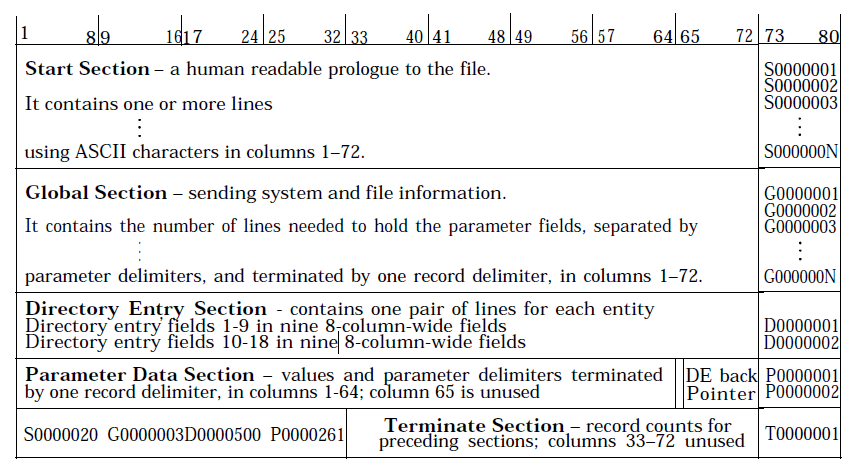
\includegraphics{literature/images/lr_iges_data_form.png}
    }
    \caption{File structure of an IGES file}
    \label{lr_fig:iges_data_form}
\end{figure}

\paragraph{}

\subsection{Non-Uniform Rational B-Spline (NURBS)}
\paragraph{}
In the proposed approach, the geometry and the unknown fields are represented by non-uniform rational B-splines (NURBS).
In this section, we give a brief overview of NURBS.
For more detailed description and implementation aspects, interested readers can refer to \cite{Pie1997,NGUYEN201589}.
\paragraph{}
% basis function
NURBS are the superset of B-spline functions.
B-spline is short for basis spline and is a generalization of Bézier curves.
A spline function is a piecewise polynomial function of degree $p$ and the points of intersection of such functions are called knots.
The number of knots must be equal to or greater than $p + 1$.
One of the salient features of spline functions is that the functions are continuous at the knots, however, the continuity of the functions can be altered by repeating the knots.
The B-spline functions are parametric functions of the form $F(\eta)$ in which the parameter $\eta$ lies in the parametric space.
The key ingredients in the construction of B-spline functions are: the knot vector (a non decreasing sequence of parameter values, $\eta_i \leq \eta_{i+1}$ , $i = 0,1,\dots,m -1$) and the degree of the curve p. The $i$th B-spline basis function of degree $p$, denoted by $_{i,p}$ is defined as \cite{Pie1997}:
\begin{equation}
    \begin{aligned}
        N_{i,0}(\eta) &=
            \begin{cases}
                1   & \text{if } \eta_i \leq \eta \leq \eta_{i+1}    \\
                0   & \text{else}
            \end{cases}\\
        N_{i,p}(\eta) &= 
            \frac{\eta - \eta_i}{\eta_{i+p}-\eta_i}     N_{i,p-1}(\eta) - 
            \frac{\eta_{i+p+1}-\eta}{\eta_{i+p+1} - \eta_{i+1}}     N_{i+1,p-1}(\eta)
    \end{aligned}
    \label{lr_nurbs_basis}
\end{equation}

The first derivative of the B-spline basis function can be computed recursively from lower order basis functions as:
\begin{equation}
    \frac{d}{d\eta} N_{i,p}(\eta) =
        \frac{p}{\eta_{i+p} - \eta_i} N_{i,p-1}(\eta) -
        \frac{p}{\eta_{i+p+1} - \eta_{i+1}} N_{i+1,p-1}(\eta)
\end{equation}

\paragraph{}
% basis properties
The B-spline basis functions has the following properties:
\begin{enumerate}
    \item Non-negativity
    \item Partition of unity, $\sum_i N_{i,p}=1$
    \item Interpolatory at the end points. The last point requires special treatment when imposing non-homogeneous Dirichlet boundary conditions [58].
\end{enumerate}


\paragraph{}
% curves
Moreover, the spline function has limited support.
Given $n + 1$ control points $(P_0 ,P_1,\dots,P_n )$ and a knot vector 
    $\Xi$ = $\left\{
        \eta_0 ,\eta_1 ,\dots,\eta_m 
    \right\}$, the piecewise polynomial B-spline curve of degree p is defined as:
\begin{equation}
    C(\eta) = \sum_{i=0}^n P_i N_{i,p} (\eta)
\end{equation}

where $P_i$ are the control points.
A B-spline curve has the following information: $n+1$ control points, $m+1$ knots and a degree $p$.
It is noted that $n$,$m$ and $p$ must satisfy $m = n + p + 1$.
The B-spline functions also provide a variety of refinement algorithms, which are essential when employing B-spline functions to discretize the unknown fields.
The analogous $h$ and $p$ refinement can be done by the process of `knot insertion' and `order elevation'.
Another unique feature of the B-spline basis function is that, it is possible to combine the knot insertion and the degree elevation, commonly referred to as ‘k-refinement’ in the literature \cite{Hug2005b}.
Here we briefly discuss the knot insertion and the degree elevation.
For more details, interested readers are referred to \cite{Pie1997,Hug2005b} and references therein.


\subsubsection{Knot insertion}
\label{lr_sec:nurbs_knot_ins}
\paragraph{}
Consider a B-spline basis functions defined on 
$\Xi = \left\{
    \eta_0 ,\eta_1,\dots,\eta_m 
    \right\}$,
let $\overline{\eta} \in [\eta_k ,\eta_{k+1} )$, and insert $\overline{\eta}$ into $\Xi$ to form a new knot vector 
$\overline{\Xi} = \left\{
    \eta_0 ,\dots, \overline{\eta}_k = \eta_k , 
    \overline{\eta}_{k+1} = \overline{\eta}, 
    \overline{\eta}_{k+2} = \overline{\eta}_{k+1} ,
    \dots,\eta_{m+1} = \eta_m
    \right\}$.
Simultaneously, the size of the control points is increased by one. Thus $C(\eta)$ has a representation on $\overline{\Xi}$ of the form
\begin{equation}
    \mathbf{C}(\eta) = \sum_{i=0}^{n+1}
                        \overline{N}_{i,p} (\eta)
                        \mathbf{Q}_i
\end{equation}
Where $\mathbf{Q}_i$ is:
\begin{equation}
    \mathbf{Q}_i = \alpha_i \mathbf{P}_i +
                    (1-\alpha_i) \mathbf{P}_{i-1}
\end{equation}
where
\begin{equation}
    \alpha_i =  \begin{cases}
                    1       & i \leq k-p \\
                    \frac{ \overline{\eta} -\eta_i }{ \eta_{i+p} - \eta_i } & k-p \leq i \leq k \\
                    0 & i \geq k+1                          
                \end{cases}
\end{equation}


\subsubsection{Order elevation}
Let $
\mathbf{C}(\eta) =  \sum_{i=0}^n
                    N_{i,p}(\eta)
                    \mathbf{P}_i
$
be a $p$th-degree B-spline curve on the knot vector $\Xi$.
As a piecewise polynomial curve with $p+1$ order, $\mathbf{C}(\eta)$ is expected to be expressed in higher order basis functions.
In other words, another set of control points $Q_i$ and knot vector $\Xi$ should exists such that
\begin{equation}
    \mathbf{C}(\eta) =  \sum_{i=0}^{\overline{n}}
                        N_{i, p+1}(\eta)
                        \mathbf{Q}_i
\end{equation}
The procedure to elevate the order of a B-spline is listed as follows \cite{Pie1997}:
\begin{enumerate}
    \item Extract each Bézier segment from the curve
    \item Elevate the order of each Bézier segment
    \item Remove unnecessary knots separating the ($i-1$)th and $i$th segments
\end{enumerate}
When elevating a $p$th Bézier curve, a new set of control points can be determined from:
\begin{equation}
    \mathbf{Q}_i =  (1-\alpha_i) \mathbf{P}_i +
                    \alpha_i \mathbf{P}_{i-1}
\end{equation}
where $\alpha_i=\frac{i}{p+i}$, $i=0$, $\dots$, $p+1$.
Fig.~\ref{lr_fig:nurbs_knotins} and Fig.~\ref{lr_fig:nurbs_orderele} show an example of basis function when performing a knot insertion and order elevation, respectively.

\begin{figure}[h!]
    \centering
    % This file was created by matlab2tikz v0.4.6 running on MATLAB 8.0.
% Copyright (c) 2008--2014, Nico Schlömer <nico.schloemer@gmail.com>
% All rights reserved.
% Minimal pgfplots version: 1.3
% 
% The latest updates can be retrieved from
%   http://www.mathworks.com/matlabcentral/fileexchange/22022-matlab2tikz
% where you can also make suggestions and rate matlab2tikz.
% 
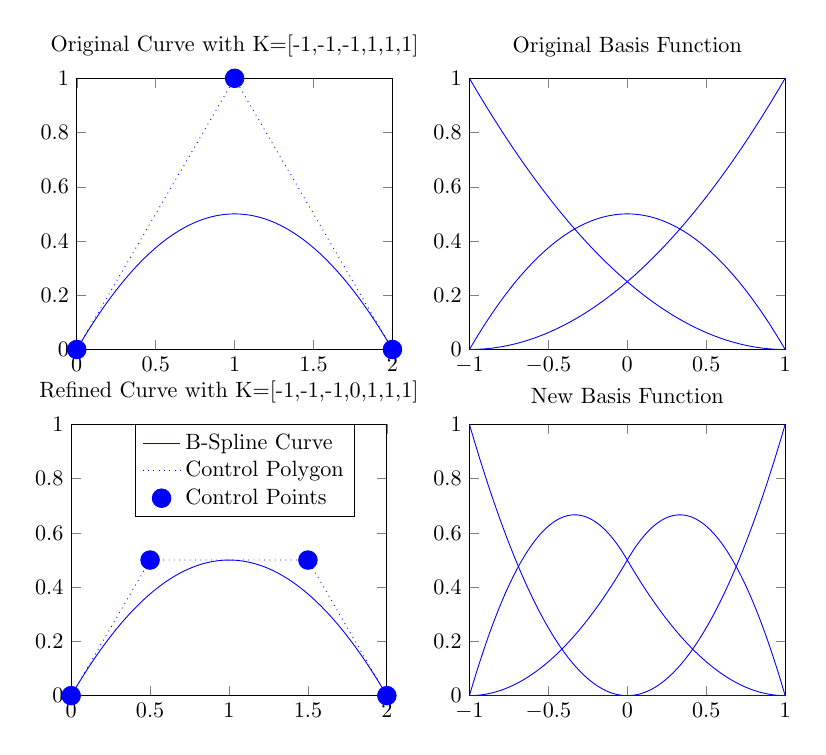
\begin{tikzpicture}[scale=0.8]

\begin{axis}[%
width=1.97309422348485in,
height=1.69505450581395in,
scale only axis,
xmin=0,
xmax=2,
ymin=0,
ymax=1,
name=plot1,
title={Original Curve with K=[-1,-1,-1,1,1,1]}
]
\addplot [color=blue,solid,forget plot]
  table[row sep=crcr]{
0	0	\\
0.0100502512562815	0.00999974748112426	\\
0.0201005025125628	0.019898487411934	\\
0.0301507537688442	0.0296962197924295	\\
0.0402010050251256	0.0393929446226105	\\
0.050251256281407	0.0489886619024772	\\
0.0603015075376885	0.0584833716320295	\\
0.0703517587939698	0.0678770738112674	\\
0.0804020100502513	0.0771697684401909	\\
0.0904522613065326	0.0863614555188	\\
0.100502512562814	0.0954521350470948	\\
0.110552763819096	0.104441807025075	\\
0.120603015075377	0.113330471452741	\\
0.130653266331658	0.122118128330093	\\
0.14070351758794	0.13080477765713	\\
0.150753768844221	0.139390419433853	\\
0.160804020100503	0.147875053660261	\\
0.170854271356784	0.156258680336355	\\
0.180904522613065	0.164541299462135	\\
0.190954773869347	0.1727229110376	\\
0.201005025125628	0.180803515062751	\\
0.21105527638191	0.188783111537587	\\
0.221105527638191	0.19666170046211	\\
0.231155778894472	0.204439281836317	\\
0.241206030150754	0.212115855660211	\\
0.251256281407035	0.21969142193379	\\
0.261306532663317	0.227165980657054	\\
0.271356783919598	0.234539531830004	\\
0.281407035175879	0.24181207545264	\\
0.291457286432161	0.248983611524961	\\
0.301507537688442	0.256054140046968	\\
0.311557788944724	0.263023661018661	\\
0.321608040201005	0.269892174440039	\\
0.331658291457286	0.276659680311103	\\
0.341708542713568	0.283326178631853	\\
0.351758793969849	0.289891669402288	\\
0.361809045226131	0.296356152622409	\\
0.371859296482412	0.302719628292215	\\
0.381909547738693	0.308982096411707	\\
0.391959798994975	0.315143556980884	\\
0.402010050251256	0.321204009999747	\\
0.412060301507538	0.327163455468296	\\
0.422110552763819	0.333021893386531	\\
0.4321608040201	0.338779323754451	\\
0.442211055276382	0.344435746572056	\\
0.452261306532663	0.349991161839347	\\
0.462311557788945	0.355445569556324	\\
0.472361809045226	0.360798969722987	\\
0.482412060301508	0.366051362339335	\\
0.492462311557789	0.371202747405369	\\
0.50251256281407	0.376253124921088	\\
0.512562814070352	0.381202494886493	\\
0.522613065326633	0.386050857301583	\\
0.532663316582915	0.390798212166359	\\
0.542713567839196	0.395444559480821	\\
0.552763819095477	0.399989899244969	\\
0.562814070351759	0.404434231458802	\\
0.57286432160804	0.40877755612232	\\
0.582914572864322	0.413019873235524	\\
0.592964824120603	0.417161182798414	\\
0.603015075376884	0.42120148481099	\\
0.613065326633166	0.425140779273251	\\
0.623115577889447	0.428979066185197	\\
0.633165829145729	0.43271634554683	\\
0.64321608040201	0.436352617358148	\\
0.653266331658292	0.439887881619151	\\
0.663316582914573	0.44332213832984	\\
0.673366834170854	0.446655387490215	\\
0.683417085427136	0.449887629100275	\\
0.693467336683417	0.453018863160021	\\
0.703517587939699	0.456049089669453	\\
0.71356783919598	0.45897830862857	\\
0.723618090452261	0.461806520037373	\\
0.733668341708543	0.464533723895861	\\
0.743718592964824	0.467159920204035	\\
0.753768844221106	0.469685108961895	\\
0.763819095477387	0.47210929016944	\\
0.773869346733668	0.474432463826671	\\
0.78391959798995	0.476654629933588	\\
0.793969849246231	0.47877578849019	\\
0.804020100502513	0.480795939496477	\\
0.814070351758794	0.482715082952451	\\
0.824120603015075	0.48453321885811	\\
0.834170854271357	0.486250347213454	\\
0.844221105527638	0.487866468018484	\\
0.85427135678392	0.4893815812732	\\
0.864321608040201	0.490795686977602	\\
0.874371859296482	0.492108785131689	\\
0.884422110552764	0.493320875735461	\\
0.894472361809045	0.494431958788919	\\
0.904522613065327	0.495442034292063	\\
0.914572864321608	0.496351102244893	\\
0.924623115577889	0.497159162647408	\\
0.934673366834171	0.497866215499609	\\
0.944723618090452	0.498472260801495	\\
0.954773869346734	0.498977298553067	\\
0.964824120603015	0.499381328754324	\\
0.974874371859296	0.499684351405268	\\
0.984924623115578	0.499886366505896	\\
0.994974874371859	0.499987374056211	\\
1.00502512562814	0.499987374056211	\\
1.01507537688442	0.499886366505896	\\
1.0251256281407	0.499684351405268	\\
1.03517587939699	0.499381328754324	\\
1.04522613065327	0.498977298553067	\\
1.05527638190955	0.498472260801495	\\
1.06532663316583	0.497866215499609	\\
1.07537688442211	0.497159162647408	\\
1.08542713567839	0.496351102244893	\\
1.09547738693467	0.495442034292063	\\
1.10552763819095	0.494431958788919	\\
1.11557788944724	0.493320875735461	\\
1.12562814070352	0.492108785131689	\\
1.1356783919598	0.490795686977602	\\
1.14572864321608	0.4893815812732	\\
1.15577889447236	0.487866468018484	\\
1.16582914572864	0.486250347213454	\\
1.17587939698492	0.48453321885811	\\
1.18592964824121	0.482715082952451	\\
1.19597989949749	0.480795939496477	\\
1.20603015075377	0.47877578849019	\\
1.21608040201005	0.476654629933588	\\
1.22613065326633	0.474432463826671	\\
1.23618090452261	0.47210929016944	\\
1.24623115577889	0.469685108961895	\\
1.25628140703518	0.467159920204035	\\
1.26633165829146	0.464533723895861	\\
1.27638190954774	0.461806520037373	\\
1.28643216080402	0.45897830862857	\\
1.2964824120603	0.456049089669453	\\
1.30653266331658	0.453018863160021	\\
1.31658291457286	0.449887629100275	\\
1.32663316582915	0.446655387490215	\\
1.33668341708543	0.44332213832984	\\
1.34673366834171	0.439887881619151	\\
1.35678391959799	0.436352617358148	\\
1.36683417085427	0.43271634554683	\\
1.37688442211055	0.428979066185197	\\
1.38693467336683	0.425140779273251	\\
1.39698492462312	0.42120148481099	\\
1.4070351758794	0.417161182798414	\\
1.41708542713568	0.413019873235524	\\
1.42713567839196	0.40877755612232	\\
1.43718592964824	0.404434231458802	\\
1.44723618090452	0.399989899244969	\\
1.4572864321608	0.395444559480821	\\
1.46733668341709	0.390798212166359	\\
1.47738693467337	0.386050857301583	\\
1.48743718592965	0.381202494886493	\\
1.49748743718593	0.376253124921088	\\
1.50753768844221	0.371202747405369	\\
1.51758793969849	0.366051362339335	\\
1.52763819095477	0.360798969722987	\\
1.53768844221106	0.355445569556324	\\
1.54773869346734	0.349991161839347	\\
1.55778894472362	0.344435746572056	\\
1.5678391959799	0.338779323754451	\\
1.57788944723618	0.333021893386531	\\
1.58793969849246	0.327163455468296	\\
1.59798994974874	0.321204009999747	\\
1.60804020100503	0.315143556980884	\\
1.61809045226131	0.308982096411707	\\
1.62814070351759	0.302719628292215	\\
1.63819095477387	0.296356152622409	\\
1.64824120603015	0.289891669402288	\\
1.65829145728643	0.283326178631853	\\
1.66834170854271	0.276659680311103	\\
1.67839195979899	0.269892174440039	\\
1.68844221105528	0.263023661018661	\\
1.69849246231156	0.256054140046968	\\
1.70854271356784	0.248983611524961	\\
1.71859296482412	0.24181207545264	\\
1.7286432160804	0.234539531830004	\\
1.73869346733668	0.227165980657054	\\
1.74874371859296	0.21969142193379	\\
1.75879396984925	0.212115855660211	\\
1.76884422110553	0.204439281836317	\\
1.77889447236181	0.19666170046211	\\
1.78894472361809	0.188783111537587	\\
1.79899497487437	0.180803515062751	\\
1.80904522613065	0.1727229110376	\\
1.81909547738693	0.164541299462135	\\
1.82914572864322	0.156258680336355	\\
1.8391959798995	0.147875053660261	\\
1.84924623115578	0.139390419433853	\\
1.85929648241206	0.13080477765713	\\
1.86934673366834	0.122118128330093	\\
1.87939698492462	0.113330471452741	\\
1.8894472361809	0.104441807025075	\\
1.89949748743719	0.0954521350470948	\\
1.90954773869347	0.0863614555188	\\
1.91959798994975	0.0771697684401908	\\
1.92964824120603	0.0678770738112675	\\
1.93969849246231	0.0584833716320295	\\
1.94974874371859	0.0489886619024772	\\
1.95979899497487	0.0393929446226105	\\
1.96984924623116	0.0296962197924294	\\
1.97989949748744	0.0198984874119341	\\
1.98994974874372	0.00999974748112426	\\
2	0	\\
};
\addplot [color=blue,dotted,forget plot]
  table[row sep=crcr]{
0	0	\\
1	1	\\
2	0	\\
};
\addplot [color=blue,mark size=4.2pt,only marks,mark=*,mark options={solid},forget plot]
  table[row sep=crcr]{
0	0	\\
1	1	\\
2	0	\\
};
\end{axis}

\begin{axis}[%
width=1.97309422348485in,
height=1.69505450581395in,
scale only axis,
xmin=-1,
xmax=1,
ymin=0,
ymax=1,
name=plot2,
at=(plot1.right of south east),
anchor=left of south west,
title={Original Basis Function}
]
\addplot [color=blue,solid,forget plot]
  table[row sep=crcr]{
-1	1	\\
-0.989949748743719	0.989975000631297	\\
-0.979899497487437	0.980000505037751	\\
-0.969849246231156	0.970076513219363	\\
-0.959798994974874	0.960203025176132	\\
-0.949748743718593	0.950380040908058	\\
-0.939698492462312	0.940607560415141	\\
-0.92964824120603	0.930885583697381	\\
-0.919597989949749	0.921214110754779	\\
-0.909547738693467	0.911593141587334	\\
-0.899497487437186	0.902022676195046	\\
-0.889447236180904	0.892502714577915	\\
-0.879396984924623	0.883033256735941	\\
-0.869346733668342	0.873614302669125	\\
-0.85929648241206	0.864245852377465	\\
-0.849246231155779	0.854927905860963	\\
-0.839195979899497	0.845660463119618	\\
-0.829145728643216	0.83644352415343	\\
-0.819095477386935	0.8272770889624	\\
-0.809045226130653	0.818161157546527	\\
-0.798994974874372	0.80909572990581	\\
-0.78894472361809	0.800080806040251	\\
-0.778894472361809	0.79111638594985	\\
-0.768844221105528	0.782202469634605	\\
-0.758793969849246	0.773339057094518	\\
-0.748743718592965	0.764526148329588	\\
-0.738693467336683	0.755763743339815	\\
-0.728643216080402	0.747051842125199	\\
-0.718592964824121	0.73839044468574	\\
-0.708542713567839	0.729779551021439	\\
-0.698492462311558	0.721219161132295	\\
-0.688442211055276	0.712709275018308	\\
-0.678391959798995	0.704249892679478	\\
-0.668341708542714	0.695841014115805	\\
-0.658291457286432	0.68748263932729	\\
-0.648241206030151	0.679174768313932	\\
-0.638190954773869	0.67091740107573	\\
-0.628140703517588	0.662710537612687	\\
-0.618090452261307	0.6545541779248	\\
-0.608040201005025	0.64644832201207	\\
-0.597989949748744	0.638392969874498	\\
-0.587939698492462	0.630388121512083	\\
-0.577889447236181	0.622433776924825	\\
-0.5678391959799	0.614529936112725	\\
-0.557788944723618	0.606676599075781	\\
-0.547738693467337	0.598873765813995	\\
-0.537688442211055	0.591121436327365	\\
-0.527638190954774	0.583419610615894	\\
-0.517587939698492	0.575768288679579	\\
-0.507537688442211	0.568167470518421	\\
-0.49748743718593	0.560617156132421	\\
-0.487437185929648	0.553117345521578	\\
-0.477386934673367	0.545668038685892	\\
-0.467336683417085	0.538269235625363	\\
-0.457286432160804	0.530920936339991	\\
-0.447236180904523	0.523623140829777	\\
-0.437185929648241	0.51637584909472	\\
-0.42713567839196	0.50917906113482	\\
-0.417085427135678	0.502032776950077	\\
-0.407035175879397	0.494936996540491	\\
-0.396984924623116	0.487891719906063	\\
-0.386934673366834	0.480896947046792	\\
-0.376884422110553	0.473952677962678	\\
-0.366834170854271	0.467058912653721	\\
-0.35678391959799	0.460215651119921	\\
-0.346733668341708	0.453422893361279	\\
-0.336683417085427	0.446680639377794	\\
-0.326633165829146	0.439988889169465	\\
-0.316582914572864	0.433347642736295	\\
-0.306532663316583	0.426756900078281	\\
-0.296482412060301	0.420216661195424	\\
-0.28643216080402	0.413726926087725	\\
-0.276381909547739	0.407287694755183	\\
-0.266331658291457	0.400898967197798	\\
-0.256281407035176	0.39456074341557	\\
-0.246231155778894	0.3882730234085	\\
-0.236180904522613	0.382035807176586	\\
-0.226130653266332	0.37584909471983	\\
-0.21608040201005	0.369712886038231	\\
-0.206030150753769	0.36362718113179	\\
-0.195979899497487	0.357591980000505	\\
-0.185929648241206	0.351607282644378	\\
-0.175879396984925	0.345673089063407	\\
-0.165829145728643	0.339789399257595	\\
-0.155778894472362	0.333956213226939	\\
-0.14572864321608	0.32817353097144	\\
-0.135678391959799	0.322441352491099	\\
-0.125628140703518	0.316759677785915	\\
-0.115577889447236	0.311128506855887	\\
-0.105527638190955	0.305547839701018	\\
-0.0954773869346733	0.300017676321305	\\
-0.085427135678392	0.29453801671675	\\
-0.0753768844221105	0.289108860887351	\\
-0.0653266331658291	0.28373020883311	\\
-0.0552763819095478	0.278402060554026	\\
-0.0452261306532663	0.2731244160501	\\
-0.035175879396985	0.26789727532133	\\
-0.0251256281407035	0.262720638367718	\\
-0.0150753768844221	0.257594505189263	\\
-0.00502512562814073	0.252518875785965	\\
0.00502512562814061	0.247493750157824	\\
0.0150753768844221	0.242519128304841	\\
0.0251256281407035	0.237595010227014	\\
0.035175879396985	0.232721395924345	\\
0.0452261306532664	0.227898285396833	\\
0.0552763819095476	0.223125678644479	\\
0.0653266331658291	0.218403575667281	\\
0.0753768844221105	0.213731976465241	\\
0.085427135678392	0.209110881038358	\\
0.0954773869346734	0.204540289386632	\\
0.105527638190955	0.200020201510063	\\
0.115577889447236	0.195550617408651	\\
0.125628140703518	0.191131537082397	\\
0.135678391959799	0.1867629605313	\\
0.14572864321608	0.18244488775536	\\
0.155778894472362	0.178177318754577	\\
0.165829145728643	0.173960253528951	\\
0.175879396984925	0.169793692078483	\\
0.185929648241206	0.165677634403172	\\
0.195979899497488	0.161612080503018	\\
0.206030150753769	0.157597030378021	\\
0.21608040201005	0.153632484028181	\\
0.226130653266332	0.149718441453499	\\
0.236180904522613	0.145854902653973	\\
0.246231155778895	0.142041867629605	\\
0.256281407035176	0.138279336380394	\\
0.266331658291457	0.134567308906341	\\
0.276381909547739	0.130905785207444	\\
0.28643216080402	0.127294765283705	\\
0.296482412060302	0.123734249135123	\\
0.306532663316583	0.120224236761698	\\
0.316582914572864	0.11676472816343	\\
0.326633165829146	0.11335572334032	\\
0.336683417085427	0.109997222292366	\\
0.346733668341709	0.10668922501957	\\
0.35678391959799	0.103431731521931	\\
0.366834170854271	0.10022474179945	\\
0.376884422110553	0.097068255852125	\\
0.386934673366834	0.0939622736799576	\\
0.396984924623116	0.0909067952829474	\\
0.407035175879397	0.0879018206610944	\\
0.417085427135678	0.0849473498143987	\\
0.42713567839196	0.08204338274286	\\
0.437185929648241	0.0791899194464786	\\
0.447236180904523	0.0763869599252544	\\
0.457286432160804	0.0736345041791874	\\
0.467336683417085	0.0709325522082776	\\
0.477386934673367	0.0682811040125249	\\
0.487437185929648	0.0656801595919295	\\
0.49748743718593	0.0631297189464912	\\
0.507537688442211	0.0606297820762102	\\
0.517587939698492	0.0581803489810864	\\
0.527638190954774	0.0557814196611197	\\
0.537688442211055	0.0534329941163102	\\
0.547738693467337	0.0511350723466579	\\
0.557788944723618	0.0488876543521628	\\
0.567839195979899	0.0466907401328249	\\
0.577889447236181	0.0445443296886442	\\
0.587939698492462	0.0424484230196207	\\
0.597989949748744	0.0404030201257544	\\
0.608040201005025	0.0384081210070453	\\
0.618090452261306	0.0364637256634934	\\
0.628140703517588	0.0345698340950986	\\
0.638190954773869	0.0327264463018611	\\
0.648241206030151	0.0309335622837807	\\
0.658291457286432	0.0291911820408575	\\
0.668341708542713	0.0274993055730916	\\
0.678391959798995	0.0258579328804828	\\
0.688442211055276	0.0242670639630312	\\
0.698492462311558	0.0227266988207368	\\
0.708542713567839	0.0212368374535996	\\
0.71859296482412	0.0197974798616197	\\
0.728643216080402	0.0184086260447969	\\
0.738693467336683	0.0170702760031312	\\
0.748743718592965	0.0157824297366228	\\
0.758793969849246	0.0145450872452716	\\
0.768844221105528	0.0133582485290775	\\
0.778894472361809	0.0122219135880407	\\
0.78894472361809	0.0111360824221611	\\
0.798994974874372	0.0101007550314386	\\
0.809045226130653	0.00911593141587333	\\
0.819095477386935	0.00818161157546526	\\
0.829145728643216	0.0072977955102144	\\
0.839195979899497	0.00646448322012071	\\
0.849246231155779	0.00568167470518421	\\
0.85929648241206	0.00494936996540491	\\
0.869346733668342	0.0042675690007828	\\
0.879396984924623	0.0036362718113179	\\
0.889447236180904	0.00305547839701018	\\
0.899497487437186	0.00252518875785965	\\
0.909547738693467	0.00204540289386631	\\
0.919597989949749	0.00161612080503017	\\
0.92964824120603	0.00123734249135123	\\
0.939698492462312	0.000909067952829475	\\
0.949748743718593	0.000631297189464912	\\
0.959798994974874	0.000404030201257543	\\
0.969849246231156	0.000227266988207367	\\
0.979899497487437	0.000101007550314387	\\
0.989949748743719	2.52518875785967e-05	\\
1	0	\\
};
\addplot [color=blue,solid,forget plot]
  table[row sep=crcr]{
-1	0	\\
-0.989949748743719	0.00999974748112426	\\
-0.979899497487437	0.019898487411934	\\
-0.969849246231156	0.0296962197924295	\\
-0.959798994974874	0.0393929446226105	\\
-0.949748743718593	0.0489886619024772	\\
-0.939698492462312	0.0584833716320295	\\
-0.92964824120603	0.0678770738112674	\\
-0.919597989949749	0.0771697684401909	\\
-0.909547738693467	0.0863614555188	\\
-0.899497487437186	0.0954521350470948	\\
-0.889447236180904	0.104441807025075	\\
-0.879396984924623	0.113330471452741	\\
-0.869346733668342	0.122118128330093	\\
-0.85929648241206	0.13080477765713	\\
-0.849246231155779	0.139390419433853	\\
-0.839195979899497	0.147875053660261	\\
-0.829145728643216	0.156258680336355	\\
-0.819095477386935	0.164541299462135	\\
-0.809045226130653	0.1727229110376	\\
-0.798994974874372	0.180803515062751	\\
-0.78894472361809	0.188783111537587	\\
-0.778894472361809	0.19666170046211	\\
-0.768844221105528	0.204439281836317	\\
-0.758793969849246	0.212115855660211	\\
-0.748743718592965	0.21969142193379	\\
-0.738693467336683	0.227165980657054	\\
-0.728643216080402	0.234539531830004	\\
-0.718592964824121	0.24181207545264	\\
-0.708542713567839	0.248983611524961	\\
-0.698492462311558	0.256054140046968	\\
-0.688442211055276	0.263023661018661	\\
-0.678391959798995	0.269892174440039	\\
-0.668341708542714	0.276659680311103	\\
-0.658291457286432	0.283326178631853	\\
-0.648241206030151	0.289891669402288	\\
-0.638190954773869	0.296356152622409	\\
-0.628140703517588	0.302719628292215	\\
-0.618090452261307	0.308982096411707	\\
-0.608040201005025	0.315143556980884	\\
-0.597989949748744	0.321204009999747	\\
-0.587939698492462	0.327163455468296	\\
-0.577889447236181	0.333021893386531	\\
-0.5678391959799	0.338779323754451	\\
-0.557788944723618	0.344435746572056	\\
-0.547738693467337	0.349991161839347	\\
-0.537688442211055	0.355445569556324	\\
-0.527638190954774	0.360798969722987	\\
-0.517587939698492	0.366051362339335	\\
-0.507537688442211	0.371202747405369	\\
-0.49748743718593	0.376253124921088	\\
-0.487437185929648	0.381202494886493	\\
-0.477386934673367	0.386050857301583	\\
-0.467336683417085	0.390798212166359	\\
-0.457286432160804	0.395444559480821	\\
-0.447236180904523	0.399989899244969	\\
-0.437185929648241	0.404434231458802	\\
-0.42713567839196	0.40877755612232	\\
-0.417085427135678	0.413019873235524	\\
-0.407035175879397	0.417161182798414	\\
-0.396984924623116	0.42120148481099	\\
-0.386934673366834	0.425140779273251	\\
-0.376884422110553	0.428979066185197	\\
-0.366834170854271	0.43271634554683	\\
-0.35678391959799	0.436352617358148	\\
-0.346733668341708	0.439887881619151	\\
-0.336683417085427	0.44332213832984	\\
-0.326633165829146	0.446655387490215	\\
-0.316582914572864	0.449887629100275	\\
-0.306532663316583	0.453018863160021	\\
-0.296482412060301	0.456049089669453	\\
-0.28643216080402	0.45897830862857	\\
-0.276381909547739	0.461806520037373	\\
-0.266331658291457	0.464533723895861	\\
-0.256281407035176	0.467159920204035	\\
-0.246231155778894	0.469685108961895	\\
-0.236180904522613	0.47210929016944	\\
-0.226130653266332	0.474432463826671	\\
-0.21608040201005	0.476654629933588	\\
-0.206030150753769	0.47877578849019	\\
-0.195979899497487	0.480795939496477	\\
-0.185929648241206	0.482715082952451	\\
-0.175879396984925	0.48453321885811	\\
-0.165829145728643	0.486250347213454	\\
-0.155778894472362	0.487866468018484	\\
-0.14572864321608	0.4893815812732	\\
-0.135678391959799	0.490795686977602	\\
-0.125628140703518	0.492108785131689	\\
-0.115577889447236	0.493320875735461	\\
-0.105527638190955	0.494431958788919	\\
-0.0954773869346733	0.495442034292063	\\
-0.085427135678392	0.496351102244893	\\
-0.0753768844221105	0.497159162647408	\\
-0.0653266331658291	0.497866215499609	\\
-0.0552763819095478	0.498472260801495	\\
-0.0452261306532663	0.498977298553067	\\
-0.035175879396985	0.499381328754324	\\
-0.0251256281407035	0.499684351405268	\\
-0.0150753768844221	0.499886366505896	\\
-0.00502512562814073	0.499987374056211	\\
0.00502512562814061	0.499987374056211	\\
0.0150753768844221	0.499886366505896	\\
0.0251256281407035	0.499684351405268	\\
0.035175879396985	0.499381328754324	\\
0.0452261306532664	0.498977298553067	\\
0.0552763819095476	0.498472260801495	\\
0.0653266331658291	0.497866215499609	\\
0.0753768844221105	0.497159162647408	\\
0.085427135678392	0.496351102244893	\\
0.0954773869346734	0.495442034292063	\\
0.105527638190955	0.494431958788919	\\
0.115577889447236	0.493320875735461	\\
0.125628140703518	0.492108785131689	\\
0.135678391959799	0.490795686977602	\\
0.14572864321608	0.4893815812732	\\
0.155778894472362	0.487866468018484	\\
0.165829145728643	0.486250347213454	\\
0.175879396984925	0.48453321885811	\\
0.185929648241206	0.482715082952451	\\
0.195979899497488	0.480795939496477	\\
0.206030150753769	0.47877578849019	\\
0.21608040201005	0.476654629933588	\\
0.226130653266332	0.474432463826671	\\
0.236180904522613	0.47210929016944	\\
0.246231155778895	0.469685108961895	\\
0.256281407035176	0.467159920204035	\\
0.266331658291457	0.464533723895861	\\
0.276381909547739	0.461806520037373	\\
0.28643216080402	0.45897830862857	\\
0.296482412060302	0.456049089669453	\\
0.306532663316583	0.453018863160021	\\
0.316582914572864	0.449887629100275	\\
0.326633165829146	0.446655387490215	\\
0.336683417085427	0.44332213832984	\\
0.346733668341709	0.439887881619151	\\
0.35678391959799	0.436352617358148	\\
0.366834170854271	0.43271634554683	\\
0.376884422110553	0.428979066185197	\\
0.386934673366834	0.425140779273251	\\
0.396984924623116	0.42120148481099	\\
0.407035175879397	0.417161182798414	\\
0.417085427135678	0.413019873235524	\\
0.42713567839196	0.40877755612232	\\
0.437185929648241	0.404434231458802	\\
0.447236180904523	0.399989899244969	\\
0.457286432160804	0.395444559480821	\\
0.467336683417085	0.390798212166359	\\
0.477386934673367	0.386050857301583	\\
0.487437185929648	0.381202494886493	\\
0.49748743718593	0.376253124921088	\\
0.507537688442211	0.371202747405369	\\
0.517587939698492	0.366051362339335	\\
0.527638190954774	0.360798969722987	\\
0.537688442211055	0.355445569556324	\\
0.547738693467337	0.349991161839347	\\
0.557788944723618	0.344435746572056	\\
0.567839195979899	0.338779323754451	\\
0.577889447236181	0.333021893386531	\\
0.587939698492462	0.327163455468296	\\
0.597989949748744	0.321204009999747	\\
0.608040201005025	0.315143556980884	\\
0.618090452261306	0.308982096411707	\\
0.628140703517588	0.302719628292215	\\
0.638190954773869	0.296356152622409	\\
0.648241206030151	0.289891669402288	\\
0.658291457286432	0.283326178631853	\\
0.668341708542713	0.276659680311103	\\
0.678391959798995	0.269892174440039	\\
0.688442211055276	0.263023661018661	\\
0.698492462311558	0.256054140046968	\\
0.708542713567839	0.248983611524961	\\
0.71859296482412	0.24181207545264	\\
0.728643216080402	0.234539531830004	\\
0.738693467336683	0.227165980657054	\\
0.748743718592965	0.21969142193379	\\
0.758793969849246	0.212115855660211	\\
0.768844221105528	0.204439281836317	\\
0.778894472361809	0.19666170046211	\\
0.78894472361809	0.188783111537587	\\
0.798994974874372	0.180803515062751	\\
0.809045226130653	0.1727229110376	\\
0.819095477386935	0.164541299462135	\\
0.829145728643216	0.156258680336355	\\
0.839195979899497	0.147875053660261	\\
0.849246231155779	0.139390419433853	\\
0.85929648241206	0.13080477765713	\\
0.869346733668342	0.122118128330093	\\
0.879396984924623	0.113330471452741	\\
0.889447236180904	0.104441807025075	\\
0.899497487437186	0.0954521350470948	\\
0.909547738693467	0.0863614555188	\\
0.919597989949749	0.0771697684401908	\\
0.92964824120603	0.0678770738112675	\\
0.939698492462312	0.0584833716320295	\\
0.949748743718593	0.0489886619024772	\\
0.959798994974874	0.0393929446226105	\\
0.969849246231156	0.0296962197924294	\\
0.979899497487437	0.0198984874119341	\\
0.989949748743719	0.00999974748112426	\\
1	0	\\
};
\addplot [color=blue,solid,forget plot]
  table[row sep=crcr]{
-1	0	\\
-0.989949748743719	2.52518875785967e-05	\\
-0.979899497487437	0.000101007550314386	\\
-0.969849246231156	0.000227266988207369	\\
-0.959798994974874	0.000404030201257543	\\
-0.949748743718593	0.000631297189464912	\\
-0.939698492462312	0.000909067952829475	\\
-0.92964824120603	0.00123734249135123	\\
-0.919597989949749	0.00161612080503018	\\
-0.909547738693467	0.00204540289386631	\\
-0.899497487437186	0.00252518875785965	\\
-0.889447236180904	0.00305547839701018	\\
-0.879396984924623	0.00363627181131789	\\
-0.869346733668342	0.00426756900078281	\\
-0.85929648241206	0.00494936996540491	\\
-0.849246231155779	0.00568167470518421	\\
-0.839195979899497	0.00646448322012071	\\
-0.829145728643216	0.00729779551021439	\\
-0.819095477386935	0.00818161157546527	\\
-0.809045226130653	0.00911593141587333	\\
-0.798994974874372	0.0101007550314386	\\
-0.78894472361809	0.0111360824221611	\\
-0.778894472361809	0.0122219135880407	\\
-0.768844221105528	0.0133582485290775	\\
-0.758793969849246	0.0145450872452716	\\
-0.748743718592965	0.0157824297366228	\\
-0.738693467336683	0.0170702760031312	\\
-0.728643216080402	0.0184086260447969	\\
-0.718592964824121	0.0197974798616197	\\
-0.708542713567839	0.0212368374535996	\\
-0.698492462311558	0.0227266988207368	\\
-0.688442211055276	0.0242670639630312	\\
-0.678391959798995	0.0258579328804828	\\
-0.668341708542714	0.0274993055730916	\\
-0.658291457286432	0.0291911820408575	\\
-0.648241206030151	0.0309335622837807	\\
-0.638190954773869	0.0327264463018611	\\
-0.628140703517588	0.0345698340950986	\\
-0.618090452261307	0.0364637256634933	\\
-0.608040201005025	0.0384081210070453	\\
-0.597989949748744	0.0404030201257544	\\
-0.587939698492462	0.0424484230196207	\\
-0.577889447236181	0.0445443296886442	\\
-0.5678391959799	0.0466907401328249	\\
-0.557788944723618	0.0488876543521628	\\
-0.547738693467337	0.0511350723466579	\\
-0.537688442211055	0.0534329941163102	\\
-0.527638190954774	0.0557814196611197	\\
-0.517587939698492	0.0581803489810863	\\
-0.507537688442211	0.0606297820762102	\\
-0.49748743718593	0.0631297189464912	\\
-0.487437185929648	0.0656801595919295	\\
-0.477386934673367	0.0682811040125249	\\
-0.467336683417085	0.0709325522082776	\\
-0.457286432160804	0.0736345041791874	\\
-0.447236180904523	0.0763869599252544	\\
-0.437185929648241	0.0791899194464786	\\
-0.42713567839196	0.08204338274286	\\
-0.417085427135678	0.0849473498143986	\\
-0.407035175879397	0.0879018206610944	\\
-0.396984924623116	0.0909067952829474	\\
-0.386934673366834	0.0939622736799576	\\
-0.376884422110553	0.097068255852125	\\
-0.366834170854271	0.10022474179945	\\
-0.35678391959799	0.103431731521931	\\
-0.346733668341708	0.10668922501957	\\
-0.336683417085427	0.109997222292366	\\
-0.326633165829146	0.11335572334032	\\
-0.316582914572864	0.11676472816343	\\
-0.306532663316583	0.120224236761698	\\
-0.296482412060301	0.123734249135123	\\
-0.28643216080402	0.127294765283705	\\
-0.276381909547739	0.130905785207444	\\
-0.266331658291457	0.134567308906341	\\
-0.256281407035176	0.138279336380394	\\
-0.246231155778894	0.142041867629605	\\
-0.236180904522613	0.145854902653973	\\
-0.226130653266332	0.149718441453499	\\
-0.21608040201005	0.153632484028181	\\
-0.206030150753769	0.157597030378021	\\
-0.195979899497487	0.161612080503018	\\
-0.185929648241206	0.165677634403172	\\
-0.175879396984925	0.169793692078483	\\
-0.165829145728643	0.173960253528951	\\
-0.155778894472362	0.178177318754577	\\
-0.14572864321608	0.18244488775536	\\
-0.135678391959799	0.1867629605313	\\
-0.125628140703518	0.191131537082397	\\
-0.115577889447236	0.195550617408651	\\
-0.105527638190955	0.200020201510063	\\
-0.0954773869346733	0.204540289386632	\\
-0.085427135678392	0.209110881038358	\\
-0.0753768844221105	0.213731976465241	\\
-0.0653266331658291	0.218403575667281	\\
-0.0552763819095478	0.223125678644479	\\
-0.0452261306532663	0.227898285396833	\\
-0.035175879396985	0.232721395924345	\\
-0.0251256281407035	0.237595010227014	\\
-0.0150753768844221	0.242519128304841	\\
-0.00502512562814073	0.247493750157824	\\
0.00502512562814061	0.252518875785965	\\
0.0150753768844221	0.257594505189263	\\
0.0251256281407035	0.262720638367718	\\
0.035175879396985	0.26789727532133	\\
0.0452261306532664	0.2731244160501	\\
0.0552763819095476	0.278402060554026	\\
0.0653266331658291	0.28373020883311	\\
0.0753768844221105	0.289108860887351	\\
0.085427135678392	0.29453801671675	\\
0.0954773869346734	0.300017676321305	\\
0.105527638190955	0.305547839701018	\\
0.115577889447236	0.311128506855887	\\
0.125628140703518	0.316759677785915	\\
0.135678391959799	0.322441352491099	\\
0.14572864321608	0.32817353097144	\\
0.155778894472362	0.333956213226939	\\
0.165829145728643	0.339789399257594	\\
0.175879396984925	0.345673089063407	\\
0.185929648241206	0.351607282644378	\\
0.195979899497488	0.357591980000505	\\
0.206030150753769	0.36362718113179	\\
0.21608040201005	0.369712886038231	\\
0.226130653266332	0.37584909471983	\\
0.236180904522613	0.382035807176586	\\
0.246231155778895	0.3882730234085	\\
0.256281407035176	0.39456074341557	\\
0.266331658291457	0.400898967197798	\\
0.276381909547739	0.407287694755183	\\
0.28643216080402	0.413726926087725	\\
0.296482412060302	0.420216661195424	\\
0.306532663316583	0.426756900078281	\\
0.316582914572864	0.433347642736295	\\
0.326633165829146	0.439988889169465	\\
0.336683417085427	0.446680639377794	\\
0.346733668341709	0.453422893361279	\\
0.35678391959799	0.460215651119921	\\
0.366834170854271	0.467058912653721	\\
0.376884422110553	0.473952677962678	\\
0.386934673366834	0.480896947046792	\\
0.396984924623116	0.487891719906063	\\
0.407035175879397	0.494936996540491	\\
0.417085427135678	0.502032776950077	\\
0.42713567839196	0.50917906113482	\\
0.437185929648241	0.51637584909472	\\
0.447236180904523	0.523623140829777	\\
0.457286432160804	0.530920936339991	\\
0.467336683417085	0.538269235625363	\\
0.477386934673367	0.545668038685892	\\
0.487437185929648	0.553117345521578	\\
0.49748743718593	0.560617156132421	\\
0.507537688442211	0.568167470518421	\\
0.517587939698492	0.575768288679579	\\
0.527638190954774	0.583419610615894	\\
0.537688442211055	0.591121436327365	\\
0.547738693467337	0.598873765813995	\\
0.557788944723618	0.606676599075781	\\
0.567839195979899	0.614529936112724	\\
0.577889447236181	0.622433776924825	\\
0.587939698492462	0.630388121512083	\\
0.597989949748744	0.638392969874498	\\
0.608040201005025	0.64644832201207	\\
0.618090452261306	0.6545541779248	\\
0.628140703517588	0.662710537612687	\\
0.638190954773869	0.67091740107573	\\
0.648241206030151	0.679174768313932	\\
0.658291457286432	0.68748263932729	\\
0.668341708542713	0.695841014115805	\\
0.678391959798995	0.704249892679478	\\
0.688442211055276	0.712709275018308	\\
0.698492462311558	0.721219161132295	\\
0.708542713567839	0.729779551021439	\\
0.71859296482412	0.73839044468574	\\
0.728643216080402	0.747051842125199	\\
0.738693467336683	0.755763743339815	\\
0.748743718592965	0.764526148329588	\\
0.758793969849246	0.773339057094518	\\
0.768844221105528	0.782202469634605	\\
0.778894472361809	0.79111638594985	\\
0.78894472361809	0.800080806040251	\\
0.798994974874372	0.80909572990581	\\
0.809045226130653	0.818161157546527	\\
0.819095477386935	0.8272770889624	\\
0.829145728643216	0.83644352415343	\\
0.839195979899497	0.845660463119618	\\
0.849246231155779	0.854927905860963	\\
0.85929648241206	0.864245852377465	\\
0.869346733668342	0.873614302669125	\\
0.879396984924623	0.883033256735941	\\
0.889447236180904	0.892502714577915	\\
0.899497487437186	0.902022676195046	\\
0.909547738693467	0.911593141587334	\\
0.919597989949749	0.921214110754779	\\
0.92964824120603	0.930885583697381	\\
0.939698492462312	0.940607560415141	\\
0.949748743718593	0.950380040908058	\\
0.959798994974874	0.960203025176132	\\
0.969849246231156	0.970076513219363	\\
0.979899497487437	0.980000505037751	\\
0.989949748743719	0.989975000631297	\\
1	1	\\
};
\end{axis}

\begin{axis}[%
width=1.97309422348485in,
height=1.69505450581395in,
scale only axis,
xmin=-1,
xmax=1,
ymin=0,
ymax=1,
name=plot4,
at=(plot2.below south west),
anchor=above north west,
title={New Basis Function}
]
\addplot [color=blue,solid,forget plot]
  table[row sep=crcr]{
-1	1	\\
-0.989949748743719	0.980000505037751	\\
-0.979899497487437	0.960203025176132	\\
-0.969849246231156	0.940607560415141	\\
-0.959798994974874	0.921214110754779	\\
-0.949748743718593	0.902022676195046	\\
-0.939698492462312	0.883033256735941	\\
-0.92964824120603	0.864245852377465	\\
-0.919597989949749	0.845660463119618	\\
-0.909547738693467	0.8272770889624	\\
-0.899497487437186	0.80909572990581	\\
-0.889447236180904	0.79111638594985	\\
-0.879396984924623	0.773339057094518	\\
-0.869346733668342	0.755763743339815	\\
-0.85929648241206	0.73839044468574	\\
-0.849246231155779	0.721219161132295	\\
-0.839195979899497	0.704249892679478	\\
-0.829145728643216	0.68748263932729	\\
-0.819095477386935	0.67091740107573	\\
-0.809045226130653	0.6545541779248	\\
-0.798994974874372	0.638392969874498	\\
-0.78894472361809	0.622433776924825	\\
-0.778894472361809	0.606676599075781	\\
-0.768844221105528	0.591121436327365	\\
-0.758793969849246	0.575768288679579	\\
-0.748743718592965	0.560617156132421	\\
-0.738693467336683	0.545668038685892	\\
-0.728643216080402	0.530920936339991	\\
-0.718592964824121	0.51637584909472	\\
-0.708542713567839	0.502032776950077	\\
-0.698492462311558	0.487891719906063	\\
-0.688442211055276	0.473952677962678	\\
-0.678391959798995	0.460215651119921	\\
-0.668341708542714	0.446680639377794	\\
-0.658291457286432	0.433347642736295	\\
-0.648241206030151	0.420216661195424	\\
-0.638190954773869	0.407287694755183	\\
-0.628140703517588	0.39456074341557	\\
-0.618090452261307	0.382035807176586	\\
-0.608040201005025	0.369712886038231	\\
-0.597989949748744	0.357591980000505	\\
-0.587939698492462	0.345673089063407	\\
-0.577889447236181	0.333956213226939	\\
-0.5678391959799	0.322441352491099	\\
-0.557788944723618	0.311128506855887	\\
-0.547738693467337	0.300017676321305	\\
-0.537688442211055	0.289108860887351	\\
-0.527638190954774	0.278402060554026	\\
-0.517587939698492	0.26789727532133	\\
-0.507537688442211	0.257594505189263	\\
-0.49748743718593	0.247493750157824	\\
-0.487437185929648	0.237595010227014	\\
-0.477386934673367	0.227898285396833	\\
-0.467336683417085	0.218403575667281	\\
-0.457286432160804	0.209110881038358	\\
-0.447236180904523	0.200020201510063	\\
-0.437185929648241	0.191131537082397	\\
-0.42713567839196	0.18244488775536	\\
-0.417085427135678	0.173960253528951	\\
-0.407035175879397	0.165677634403172	\\
-0.396984924623116	0.157597030378021	\\
-0.386934673366834	0.149718441453499	\\
-0.376884422110553	0.142041867629605	\\
-0.366834170854271	0.134567308906341	\\
-0.35678391959799	0.127294765283705	\\
-0.346733668341708	0.120224236761698	\\
-0.336683417085427	0.11335572334032	\\
-0.326633165829146	0.10668922501957	\\
-0.316582914572864	0.10022474179945	\\
-0.306532663316583	0.0939622736799576	\\
-0.296482412060301	0.0879018206610944	\\
-0.28643216080402	0.08204338274286	\\
-0.276381909547739	0.0763869599252544	\\
-0.266331658291457	0.0709325522082776	\\
-0.256281407035176	0.0656801595919295	\\
-0.246231155778894	0.0606297820762102	\\
-0.236180904522613	0.0557814196611197	\\
-0.226130653266332	0.0511350723466579	\\
-0.21608040201005	0.0466907401328249	\\
-0.206030150753769	0.0424484230196207	\\
-0.195979899497487	0.0384081210070453	\\
-0.185929648241206	0.0345698340950986	\\
-0.175879396984925	0.0309335622837807	\\
-0.165829145728643	0.0274993055730916	\\
-0.155778894472362	0.0242670639630312	\\
-0.14572864321608	0.0212368374535996	\\
-0.135678391959799	0.0184086260447969	\\
-0.125628140703518	0.0157824297366228	\\
-0.115577889447236	0.0133582485290775	\\
-0.105527638190955	0.0111360824221611	\\
-0.0954773869346733	0.00911593141587333	\\
-0.085427135678392	0.0072977955102144	\\
-0.0753768844221105	0.00568167470518421	\\
-0.0653266331658291	0.0042675690007828	\\
-0.0552763819095478	0.00305547839701018	\\
-0.0452261306532663	0.00204540289386631	\\
-0.035175879396985	0.00123734249135123	\\
-0.0251256281407035	0.000631297189464912	\\
-0.0150753768844221	0.000227266988207367	\\
-0.00502512562814073	2.52518875785967e-05	\\
0.00502512562814061	0	\\
0.0150753768844221	0	\\
0.0251256281407035	0	\\
0.035175879396985	0	\\
0.0452261306532664	0	\\
0.0552763819095476	0	\\
0.0653266331658291	0	\\
0.0753768844221105	0	\\
0.085427135678392	0	\\
0.0954773869346734	0	\\
0.105527638190955	0	\\
0.115577889447236	0	\\
0.125628140703518	0	\\
0.135678391959799	0	\\
0.14572864321608	0	\\
0.155778894472362	0	\\
0.165829145728643	0	\\
0.175879396984925	0	\\
0.185929648241206	0	\\
0.195979899497488	0	\\
0.206030150753769	0	\\
0.21608040201005	0	\\
0.226130653266332	0	\\
0.236180904522613	0	\\
0.246231155778895	0	\\
0.256281407035176	0	\\
0.266331658291457	0	\\
0.276381909547739	0	\\
0.28643216080402	0	\\
0.296482412060302	0	\\
0.306532663316583	0	\\
0.316582914572864	0	\\
0.326633165829146	0	\\
0.336683417085427	0	\\
0.346733668341709	0	\\
0.35678391959799	0	\\
0.366834170854271	0	\\
0.376884422110553	0	\\
0.386934673366834	0	\\
0.396984924623116	0	\\
0.407035175879397	0	\\
0.417085427135678	0	\\
0.42713567839196	0	\\
0.437185929648241	0	\\
0.447236180904523	0	\\
0.457286432160804	0	\\
0.467336683417085	0	\\
0.477386934673367	0	\\
0.487437185929648	0	\\
0.49748743718593	0	\\
0.507537688442211	0	\\
0.517587939698492	0	\\
0.527638190954774	0	\\
0.537688442211055	0	\\
0.547738693467337	0	\\
0.557788944723618	0	\\
0.567839195979899	0	\\
0.577889447236181	0	\\
0.587939698492462	0	\\
0.597989949748744	0	\\
0.608040201005025	0	\\
0.618090452261306	0	\\
0.628140703517588	0	\\
0.638190954773869	0	\\
0.648241206030151	0	\\
0.658291457286432	0	\\
0.668341708542713	0	\\
0.678391959798995	0	\\
0.688442211055276	0	\\
0.698492462311558	0	\\
0.708542713567839	0	\\
0.71859296482412	0	\\
0.728643216080402	0	\\
0.738693467336683	0	\\
0.748743718592965	0	\\
0.758793969849246	0	\\
0.768844221105528	0	\\
0.778894472361809	0	\\
0.78894472361809	0	\\
0.798994974874372	0	\\
0.809045226130653	0	\\
0.819095477386935	0	\\
0.829145728643216	0	\\
0.839195979899497	0	\\
0.849246231155779	0	\\
0.85929648241206	0	\\
0.869346733668342	0	\\
0.879396984924623	0	\\
0.889447236180904	0	\\
0.899497487437186	0	\\
0.909547738693467	0	\\
0.919597989949749	0	\\
0.92964824120603	0	\\
0.939698492462312	0	\\
0.949748743718593	0	\\
0.959798994974874	0	\\
0.969849246231156	0	\\
0.979899497487437	0	\\
0.989949748743719	0	\\
1	0	\\
};
\addplot [color=blue,solid,forget plot]
  table[row sep=crcr]{
-1	0	\\
-0.989949748743719	0.0199489911870913	\\
-0.979899497487437	0.0395949597232393	\\
-0.969849246231156	0.0589379056084443	\\
-0.959798994974874	0.0779778288427059	\\
-0.949748743718593	0.0967147294260246	\\
-0.939698492462312	0.1151486073584	\\
-0.92964824120603	0.133279462639832	\\
-0.919597989949749	0.151107295270321	\\
-0.909547738693467	0.168632105249867	\\
-0.899497487437186	0.18585389257847	\\
-0.889447236180904	0.20277265725613	\\
-0.879396984924623	0.219388399282846	\\
-0.869346733668342	0.23570111865862	\\
-0.85929648241206	0.25171081538345	\\
-0.849246231155779	0.267417489457337	\\
-0.839195979899497	0.282821140880281	\\
-0.829145728643216	0.297921769652281	\\
-0.819095477386935	0.312719375773339	\\
-0.809045226130653	0.327213959243453	\\
-0.798994974874372	0.341405520062625	\\
-0.78894472361809	0.355294058230853	\\
-0.778894472361809	0.368879573748138	\\
-0.768844221105528	0.382162066614479	\\
-0.758793969849246	0.395141536829878	\\
-0.748743718592965	0.407817984394333	\\
-0.738693467336683	0.420191409307846	\\
-0.728643216080402	0.432261811570415	\\
-0.718592964824121	0.444029191182041	\\
-0.708542713567839	0.455493548142724	\\
-0.698492462311558	0.466654882452463	\\
-0.688442211055276	0.47751319411126	\\
-0.678391959798995	0.488068483119113	\\
-0.668341708542714	0.498320749476023	\\
-0.658291457286432	0.50826999318199	\\
-0.648241206030151	0.517916214237014	\\
-0.638190954773869	0.527259412641095	\\
-0.628140703517588	0.536299588394233	\\
-0.618090452261307	0.545036741496427	\\
-0.608040201005025	0.553470871947678	\\
-0.597989949748744	0.561601979747986	\\
-0.587939698492462	0.569430064897351	\\
-0.577889447236181	0.576955127395773	\\
-0.5678391959799	0.584177167243251	\\
-0.557788944723618	0.591096184439787	\\
-0.547738693467337	0.597712178985379	\\
-0.537688442211055	0.604025150880028	\\
-0.527638190954774	0.610035100123734	\\
-0.517587939698492	0.615742026716497	\\
-0.507537688442211	0.621145930658317	\\
-0.49748743718593	0.626246811949193	\\
-0.487437185929648	0.631044670589127	\\
-0.477386934673367	0.635539506578117	\\
-0.467336683417085	0.639731319916164	\\
-0.457286432160804	0.643620110603268	\\
-0.447236180904523	0.647205878639428	\\
-0.437185929648241	0.650488624024646	\\
-0.42713567839196	0.65346834675892	\\
-0.417085427135678	0.656145046842252	\\
-0.407035175879397	0.65851872427464	\\
-0.396984924623116	0.660589379056084	\\
-0.386934673366834	0.662357011186586	\\
-0.376884422110553	0.663821620666145	\\
-0.366834170854271	0.66498320749476	\\
-0.35678391959799	0.665841771672433	\\
-0.346733668341708	0.666397313199162	\\
-0.336683417085427	0.666649832074948	\\
-0.326633165829146	0.66659932829979	\\
-0.316582914572864	0.66624580187369	\\
-0.306532663316583	0.665589252796646	\\
-0.296482412060301	0.66462968106866	\\
-0.28643216080402	0.66336708668973	\\
-0.276381909547739	0.661801469659857	\\
-0.266331658291457	0.659932829979041	\\
-0.256281407035176	0.657761167647282	\\
-0.246231155778894	0.655286482664579	\\
-0.236180904522613	0.652508775030934	\\
-0.226130653266332	0.649428044746345	\\
-0.21608040201005	0.646044291810813	\\
-0.206030150753769	0.642357516224338	\\
-0.195979899497487	0.63836771798692	\\
-0.185929648241206	0.634074897098558	\\
-0.175879396984925	0.629479053559253	\\
-0.165829145728643	0.624580187369006	\\
-0.155778894472362	0.619378298527815	\\
-0.14572864321608	0.613873387035681	\\
-0.135678391959799	0.608065452892604	\\
-0.125628140703518	0.601954496098583	\\
-0.115577889447236	0.59554051665362	\\
-0.105527638190955	0.588823514557713	\\
-0.0954773869346733	0.581803489810863	\\
-0.085427135678392	0.57448044241307	\\
-0.0753768844221105	0.566854372364334	\\
-0.0653266331658291	0.558925279664655	\\
-0.0552763819095478	0.550693164314032	\\
-0.0452261306532663	0.542158026312467	\\
-0.035175879396985	0.533319865659958	\\
-0.0251256281407035	0.524178682356506	\\
-0.0150753768844221	0.514734476402111	\\
-0.00502512562814073	0.504987247796773	\\
0.00502512562814061	0.494987500315649	\\
0.0150753768844221	0.485038256609682	\\
0.0251256281407035	0.475190020454029	\\
0.035175879396985	0.465442791848691	\\
0.0452261306532664	0.455796570793667	\\
0.0552763819095476	0.446251357288957	\\
0.0653266331658291	0.436807151334562	\\
0.0753768844221105	0.427463952930482	\\
0.085427135678392	0.418221762076715	\\
0.0954773869346734	0.409080578773263	\\
0.105527638190955	0.400040403020126	\\
0.115577889447236	0.391101234817303	\\
0.125628140703518	0.382263074164794	\\
0.135678391959799	0.373525921062599	\\
0.14572864321608	0.364889775510719	\\
0.155778894472362	0.356354637509154	\\
0.165829145728643	0.347920507057903	\\
0.175879396984925	0.339587384156966	\\
0.185929648241206	0.331355268806343	\\
0.195979899497488	0.323224161006035	\\
0.206030150753769	0.315194060756042	\\
0.21608040201005	0.307264968056362	\\
0.226130653266332	0.299436882906997	\\
0.236180904522613	0.291709805307947	\\
0.246231155778895	0.284083735259211	\\
0.256281407035176	0.276558672760789	\\
0.266331658291457	0.269134617812682	\\
0.276381909547739	0.261811570414889	\\
0.28643216080402	0.25458953056741	\\
0.296482412060302	0.247468498270246	\\
0.306532663316583	0.240448473523396	\\
0.316582914572864	0.23352945632686	\\
0.326633165829146	0.226711446680639	\\
0.336683417085427	0.219994444584733	\\
0.346733668341709	0.21337845003914	\\
0.35678391959799	0.206863463043862	\\
0.366834170854271	0.200449483598899	\\
0.376884422110553	0.19413651170425	\\
0.386934673366834	0.187924547359915	\\
0.396984924623116	0.181813590565895	\\
0.407035175879397	0.175803641322189	\\
0.417085427135678	0.169894699628797	\\
0.42713567839196	0.16408676548572	\\
0.437185929648241	0.158379838892957	\\
0.447236180904523	0.152773919850509	\\
0.457286432160804	0.147269008358375	\\
0.467336683417085	0.141865104416555	\\
0.477386934673367	0.13656220802505	\\
0.487437185929648	0.131360319183859	\\
0.49748743718593	0.126259437892982	\\
0.507537688442211	0.12125956415242	\\
0.517587939698492	0.116360697962173	\\
0.527638190954774	0.111562839322239	\\
0.537688442211055	0.10686598823262	\\
0.547738693467337	0.102270144693316	\\
0.557788944723618	0.0977753087043256	\\
0.567839195979899	0.0933814802656499	\\
0.577889447236181	0.0890886593772885	\\
0.587939698492462	0.0848968460392414	\\
0.597989949748744	0.0808060402515088	\\
0.608040201005025	0.0768162420140905	\\
0.618090452261306	0.0729274513269867	\\
0.628140703517588	0.0691396681901972	\\
0.638190954773869	0.0654528926037221	\\
0.648241206030151	0.0618671245675614	\\
0.658291457286432	0.0583823640817151	\\
0.668341708542713	0.0549986111461832	\\
0.678391959798995	0.0517158657609657	\\
0.688442211055276	0.0485341279260625	\\
0.698492462311558	0.0454533976414737	\\
0.708542713567839	0.0424736749071993	\\
0.71859296482412	0.0395949597232393	\\
0.728643216080402	0.0368172520895937	\\
0.738693467336683	0.0341405520062625	\\
0.748743718592965	0.0315648594732456	\\
0.758793969849246	0.0290901744905432	\\
0.768844221105528	0.0267164970581551	\\
0.778894472361809	0.0244438271760814	\\
0.78894472361809	0.0222721648443221	\\
0.798994974874372	0.0202015100628772	\\
0.809045226130653	0.0182318628317467	\\
0.819095477386935	0.0163632231509305	\\
0.829145728643216	0.0145955910204288	\\
0.839195979899497	0.0129289664402414	\\
0.849246231155779	0.0113633494103684	\\
0.85929648241206	0.00989873993080982	\\
0.869346733668342	0.0085351380015656	\\
0.879396984924623	0.0072725436226358	\\
0.889447236180904	0.00611095679402036	\\
0.899497487437186	0.0050503775157193	\\
0.909547738693467	0.00409080578773263	\\
0.919597989949749	0.00323224161006034	\\
0.92964824120603	0.00247468498270246	\\
0.939698492462312	0.00181813590565895	\\
0.949748743718593	0.00126259437892982	\\
0.959798994974874	0.000808060402515086	\\
0.969849246231156	0.000454533976414734	\\
0.979899497487437	0.000202015100628774	\\
0.989949748743719	5.05037751571934e-05	\\
1	0	\\
};
\addplot [color=blue,solid,forget plot]
  table[row sep=crcr]{
-1	0	\\
-0.989949748743719	5.05037751571934e-05	\\
-0.979899497487437	0.000202015100628772	\\
-0.969849246231156	0.000454533976414738	\\
-0.959798994974874	0.000808060402515086	\\
-0.949748743718593	0.00126259437892982	\\
-0.939698492462312	0.00181813590565895	\\
-0.92964824120603	0.00247468498270246	\\
-0.919597989949749	0.00323224161006035	\\
-0.909547738693467	0.00409080578773263	\\
-0.899497487437186	0.0050503775157193	\\
-0.889447236180904	0.00611095679402036	\\
-0.879396984924623	0.00727254362263579	\\
-0.869346733668342	0.00853513800156562	\\
-0.85929648241206	0.00989873993080982	\\
-0.849246231155779	0.0113633494103684	\\
-0.839195979899497	0.0129289664402414	\\
-0.829145728643216	0.0145955910204288	\\
-0.819095477386935	0.0163632231509305	\\
-0.809045226130653	0.0182318628317467	\\
-0.798994974874372	0.0202015100628772	\\
-0.78894472361809	0.0222721648443221	\\
-0.778894472361809	0.0244438271760814	\\
-0.768844221105528	0.0267164970581551	\\
-0.758793969849246	0.0290901744905432	\\
-0.748743718592965	0.0315648594732456	\\
-0.738693467336683	0.0341405520062625	\\
-0.728643216080402	0.0368172520895937	\\
-0.718592964824121	0.0395949597232393	\\
-0.708542713567839	0.0424736749071993	\\
-0.698492462311558	0.0454533976414737	\\
-0.688442211055276	0.0485341279260625	\\
-0.678391959798995	0.0517158657609657	\\
-0.668341708542714	0.0549986111461832	\\
-0.658291457286432	0.0583823640817151	\\
-0.648241206030151	0.0618671245675614	\\
-0.638190954773869	0.0654528926037221	\\
-0.628140703517588	0.0691396681901972	\\
-0.618090452261307	0.0729274513269867	\\
-0.608040201005025	0.0768162420140905	\\
-0.597989949748744	0.0808060402515088	\\
-0.587939698492462	0.0848968460392414	\\
-0.577889447236181	0.0890886593772885	\\
-0.5678391959799	0.0933814802656499	\\
-0.557788944723618	0.0977753087043257	\\
-0.547738693467337	0.102270144693316	\\
-0.537688442211055	0.10686598823262	\\
-0.527638190954774	0.111562839322239	\\
-0.517587939698492	0.116360697962173	\\
-0.507537688442211	0.12125956415242	\\
-0.49748743718593	0.126259437892982	\\
-0.487437185929648	0.131360319183859	\\
-0.477386934673367	0.13656220802505	\\
-0.467336683417085	0.141865104416555	\\
-0.457286432160804	0.147269008358375	\\
-0.447236180904523	0.152773919850509	\\
-0.437185929648241	0.158379838892957	\\
-0.42713567839196	0.16408676548572	\\
-0.417085427135678	0.169894699628797	\\
-0.407035175879397	0.175803641322189	\\
-0.396984924623116	0.181813590565895	\\
-0.386934673366834	0.187924547359915	\\
-0.376884422110553	0.19413651170425	\\
-0.366834170854271	0.200449483598899	\\
-0.35678391959799	0.206863463043863	\\
-0.346733668341708	0.21337845003914	\\
-0.336683417085427	0.219994444584733	\\
-0.326633165829146	0.226711446680639	\\
-0.316582914572864	0.23352945632686	\\
-0.306532663316583	0.240448473523396	\\
-0.296482412060301	0.247468498270246	\\
-0.28643216080402	0.25458953056741	\\
-0.276381909547739	0.261811570414889	\\
-0.266331658291457	0.269134617812681	\\
-0.256281407035176	0.276558672760789	\\
-0.246231155778894	0.284083735259211	\\
-0.236180904522613	0.291709805307947	\\
-0.226130653266332	0.299436882906997	\\
-0.21608040201005	0.307264968056362	\\
-0.206030150753769	0.315194060756042	\\
-0.195979899497487	0.323224161006035	\\
-0.185929648241206	0.331355268806343	\\
-0.175879396984925	0.339587384156966	\\
-0.165829145728643	0.347920507057903	\\
-0.155778894472362	0.356354637509154	\\
-0.14572864321608	0.364889775510719	\\
-0.135678391959799	0.373525921062599	\\
-0.125628140703518	0.382263074164794	\\
-0.115577889447236	0.391101234817303	\\
-0.105527638190955	0.400040403020126	\\
-0.0954773869346733	0.409080578773263	\\
-0.085427135678392	0.418221762076715	\\
-0.0753768844221105	0.427463952930482	\\
-0.0653266331658291	0.436807151334562	\\
-0.0552763819095478	0.446251357288957	\\
-0.0452261306532663	0.455796570793667	\\
-0.035175879396985	0.465442791848691	\\
-0.0251256281407035	0.475190020454029	\\
-0.0150753768844221	0.485038256609682	\\
-0.00502512562814073	0.494987500315649	\\
0.00502512562814061	0.504987247796773	\\
0.0150753768844221	0.514734476402111	\\
0.0251256281407035	0.524178682356506	\\
0.035175879396985	0.533319865659958	\\
0.0452261306532664	0.542158026312467	\\
0.0552763819095476	0.550693164314032	\\
0.0653266331658291	0.558925279664655	\\
0.0753768844221105	0.566854372364334	\\
0.085427135678392	0.57448044241307	\\
0.0954773869346734	0.581803489810863	\\
0.105527638190955	0.588823514557713	\\
0.115577889447236	0.59554051665362	\\
0.125628140703518	0.601954496098583	\\
0.135678391959799	0.608065452892604	\\
0.14572864321608	0.613873387035681	\\
0.155778894472362	0.619378298527815	\\
0.165829145728643	0.624580187369006	\\
0.175879396984925	0.629479053559253	\\
0.185929648241206	0.634074897098558	\\
0.195979899497488	0.63836771798692	\\
0.206030150753769	0.642357516224338	\\
0.21608040201005	0.646044291810813	\\
0.226130653266332	0.649428044746345	\\
0.236180904522613	0.652508775030934	\\
0.246231155778895	0.655286482664579	\\
0.256281407035176	0.657761167647282	\\
0.266331658291457	0.659932829979041	\\
0.276381909547739	0.661801469659857	\\
0.28643216080402	0.66336708668973	\\
0.296482412060302	0.66462968106866	\\
0.306532663316583	0.665589252796646	\\
0.316582914572864	0.66624580187369	\\
0.326633165829146	0.66659932829979	\\
0.336683417085427	0.666649832074948	\\
0.346733668341709	0.666397313199162	\\
0.35678391959799	0.665841771672433	\\
0.366834170854271	0.66498320749476	\\
0.376884422110553	0.663821620666145	\\
0.386934673366834	0.662357011186586	\\
0.396984924623116	0.660589379056084	\\
0.407035175879397	0.65851872427464	\\
0.417085427135678	0.656145046842252	\\
0.42713567839196	0.65346834675892	\\
0.437185929648241	0.650488624024646	\\
0.447236180904523	0.647205878639428	\\
0.457286432160804	0.643620110603268	\\
0.467336683417085	0.639731319916164	\\
0.477386934673367	0.635539506578117	\\
0.487437185929648	0.631044670589127	\\
0.49748743718593	0.626246811949193	\\
0.507537688442211	0.621145930658317	\\
0.517587939698492	0.615742026716497	\\
0.527638190954774	0.610035100123734	\\
0.537688442211055	0.604025150880028	\\
0.547738693467337	0.597712178985379	\\
0.557788944723618	0.591096184439787	\\
0.567839195979899	0.584177167243252	\\
0.577889447236181	0.576955127395773	\\
0.587939698492462	0.569430064897351	\\
0.597989949748744	0.561601979747986	\\
0.608040201005025	0.553470871947678	\\
0.618090452261306	0.545036741496427	\\
0.628140703517588	0.536299588394233	\\
0.638190954773869	0.527259412641095	\\
0.648241206030151	0.517916214237014	\\
0.658291457286432	0.50826999318199	\\
0.668341708542713	0.498320749476023	\\
0.678391959798995	0.488068483119113	\\
0.688442211055276	0.47751319411126	\\
0.698492462311558	0.466654882452463	\\
0.708542713567839	0.455493548142724	\\
0.71859296482412	0.444029191182041	\\
0.728643216080402	0.432261811570415	\\
0.738693467336683	0.420191409307846	\\
0.748743718592965	0.407817984394333	\\
0.758793969849246	0.395141536829878	\\
0.768844221105528	0.382162066614479	\\
0.778894472361809	0.368879573748138	\\
0.78894472361809	0.355294058230853	\\
0.798994974874372	0.341405520062625	\\
0.809045226130653	0.327213959243453	\\
0.819095477386935	0.312719375773339	\\
0.829145728643216	0.297921769652282	\\
0.839195979899497	0.282821140880281	\\
0.849246231155779	0.267417489457337	\\
0.85929648241206	0.25171081538345	\\
0.869346733668342	0.23570111865862	\\
0.879396984924623	0.219388399282847	\\
0.889447236180904	0.20277265725613	\\
0.899497487437186	0.18585389257847	\\
0.909547738693467	0.168632105249867	\\
0.919597989949749	0.151107295270321	\\
0.92964824120603	0.133279462639832	\\
0.939698492462312	0.1151486073584	\\
0.949748743718593	0.0967147294260246	\\
0.959798994974874	0.0779778288427059	\\
0.969849246231156	0.0589379056084441	\\
0.979899497487437	0.0395949597232395	\\
0.989949748743719	0.0199489911870913	\\
1	0	\\
};
\addplot [color=blue,solid,forget plot]
  table[row sep=crcr]{
-1	0	\\
-0.989949748743719	0	\\
-0.979899497487437	0	\\
-0.969849246231156	0	\\
-0.959798994974874	0	\\
-0.949748743718593	0	\\
-0.939698492462312	0	\\
-0.92964824120603	0	\\
-0.919597989949749	0	\\
-0.909547738693467	0	\\
-0.899497487437186	0	\\
-0.889447236180904	0	\\
-0.879396984924623	0	\\
-0.869346733668342	0	\\
-0.85929648241206	0	\\
-0.849246231155779	0	\\
-0.839195979899497	0	\\
-0.829145728643216	0	\\
-0.819095477386935	0	\\
-0.809045226130653	0	\\
-0.798994974874372	0	\\
-0.78894472361809	0	\\
-0.778894472361809	0	\\
-0.768844221105528	0	\\
-0.758793969849246	0	\\
-0.748743718592965	0	\\
-0.738693467336683	0	\\
-0.728643216080402	0	\\
-0.718592964824121	0	\\
-0.708542713567839	0	\\
-0.698492462311558	0	\\
-0.688442211055276	0	\\
-0.678391959798995	0	\\
-0.668341708542714	0	\\
-0.658291457286432	0	\\
-0.648241206030151	0	\\
-0.638190954773869	0	\\
-0.628140703517588	0	\\
-0.618090452261307	0	\\
-0.608040201005025	0	\\
-0.597989949748744	0	\\
-0.587939698492462	0	\\
-0.577889447236181	0	\\
-0.5678391959799	0	\\
-0.557788944723618	0	\\
-0.547738693467337	0	\\
-0.537688442211055	0	\\
-0.527638190954774	0	\\
-0.517587939698492	0	\\
-0.507537688442211	0	\\
-0.49748743718593	0	\\
-0.487437185929648	0	\\
-0.477386934673367	0	\\
-0.467336683417085	0	\\
-0.457286432160804	0	\\
-0.447236180904523	0	\\
-0.437185929648241	0	\\
-0.42713567839196	0	\\
-0.417085427135678	0	\\
-0.407035175879397	0	\\
-0.396984924623116	0	\\
-0.386934673366834	0	\\
-0.376884422110553	0	\\
-0.366834170854271	0	\\
-0.35678391959799	0	\\
-0.346733668341708	0	\\
-0.336683417085427	0	\\
-0.326633165829146	0	\\
-0.316582914572864	0	\\
-0.306532663316583	0	\\
-0.296482412060301	0	\\
-0.28643216080402	0	\\
-0.276381909547739	0	\\
-0.266331658291457	0	\\
-0.256281407035176	0	\\
-0.246231155778894	0	\\
-0.236180904522613	0	\\
-0.226130653266332	0	\\
-0.21608040201005	0	\\
-0.206030150753769	0	\\
-0.195979899497487	0	\\
-0.185929648241206	0	\\
-0.175879396984925	0	\\
-0.165829145728643	0	\\
-0.155778894472362	0	\\
-0.14572864321608	0	\\
-0.135678391959799	0	\\
-0.125628140703518	0	\\
-0.115577889447236	0	\\
-0.105527638190955	0	\\
-0.0954773869346733	0	\\
-0.085427135678392	0	\\
-0.0753768844221105	0	\\
-0.0653266331658291	0	\\
-0.0552763819095478	0	\\
-0.0452261306532663	0	\\
-0.035175879396985	0	\\
-0.0251256281407035	0	\\
-0.0150753768844221	0	\\
-0.00502512562814073	0	\\
0.00502512562814061	2.52518875785956e-05	\\
0.0150753768844221	0.000227266988207367	\\
0.0251256281407035	0.000631297189464912	\\
0.035175879396985	0.00123734249135123	\\
0.0452261306532664	0.00204540289386632	\\
0.0552763819095476	0.00305547839701017	\\
0.0653266331658291	0.0042675690007828	\\
0.0753768844221105	0.00568167470518421	\\
0.085427135678392	0.0072977955102144	\\
0.0954773869346734	0.00911593141587335	\\
0.105527638190955	0.011136082422161	\\
0.115577889447236	0.0133582485290775	\\
0.125628140703518	0.0157824297366228	\\
0.135678391959799	0.0184086260447969	\\
0.14572864321608	0.0212368374535997	\\
0.155778894472362	0.0242670639630312	\\
0.165829145728643	0.0274993055730916	\\
0.175879396984925	0.0309335622837807	\\
0.185929648241206	0.0345698340950986	\\
0.195979899497488	0.0384081210070453	\\
0.206030150753769	0.0424484230196207	\\
0.21608040201005	0.0466907401328249	\\
0.226130653266332	0.0511350723466579	\\
0.236180904522613	0.0557814196611197	\\
0.246231155778895	0.0606297820762102	\\
0.256281407035176	0.0656801595919295	\\
0.266331658291457	0.0709325522082775	\\
0.276381909547739	0.0763869599252544	\\
0.28643216080402	0.08204338274286	\\
0.296482412060302	0.0879018206610944	\\
0.306532663316583	0.0939622736799576	\\
0.316582914572864	0.100224741799449	\\
0.326633165829146	0.10668922501957	\\
0.336683417085427	0.11335572334032	\\
0.346733668341709	0.120224236761698	\\
0.35678391959799	0.127294765283705	\\
0.366834170854271	0.134567308906341	\\
0.376884422110553	0.142041867629605	\\
0.386934673366834	0.149718441453499	\\
0.396984924623116	0.157597030378021	\\
0.407035175879397	0.165677634403172	\\
0.417085427135678	0.173960253528951	\\
0.42713567839196	0.18244488775536	\\
0.437185929648241	0.191131537082397	\\
0.447236180904523	0.200020201510063	\\
0.457286432160804	0.209110881038358	\\
0.467336683417085	0.218403575667281	\\
0.477386934673367	0.227898285396833	\\
0.487437185929648	0.237595010227014	\\
0.49748743718593	0.247493750157824	\\
0.507537688442211	0.257594505189263	\\
0.517587939698492	0.26789727532133	\\
0.527638190954774	0.278402060554026	\\
0.537688442211055	0.289108860887351	\\
0.547738693467337	0.300017676321305	\\
0.557788944723618	0.311128506855888	\\
0.567839195979899	0.322441352491099	\\
0.577889447236181	0.333956213226939	\\
0.587939698492462	0.345673089063407	\\
0.597989949748744	0.357591980000505	\\
0.608040201005025	0.369712886038231	\\
0.618090452261306	0.382035807176586	\\
0.628140703517588	0.39456074341557	\\
0.638190954773869	0.407287694755183	\\
0.648241206030151	0.420216661195424	\\
0.658291457286432	0.433347642736295	\\
0.668341708542713	0.446680639377793	\\
0.678391959798995	0.460215651119921	\\
0.688442211055276	0.473952677962678	\\
0.698492462311558	0.487891719906063	\\
0.708542713567839	0.502032776950077	\\
0.71859296482412	0.51637584909472	\\
0.728643216080402	0.530920936339991	\\
0.738693467336683	0.545668038685892	\\
0.748743718592965	0.560617156132421	\\
0.758793969849246	0.575768288679579	\\
0.768844221105528	0.591121436327366	\\
0.778894472361809	0.606676599075781	\\
0.78894472361809	0.622433776924825	\\
0.798994974874372	0.638392969874498	\\
0.809045226130653	0.6545541779248	\\
0.819095477386935	0.670917401075731	\\
0.829145728643216	0.68748263932729	\\
0.839195979899497	0.704249892679478	\\
0.849246231155779	0.721219161132295	\\
0.85929648241206	0.73839044468574	\\
0.869346733668342	0.755763743339815	\\
0.879396984924623	0.773339057094518	\\
0.889447236180904	0.79111638594985	\\
0.899497487437186	0.80909572990581	\\
0.909547738693467	0.8272770889624	\\
0.919597989949749	0.845660463119618	\\
0.92964824120603	0.864245852377465	\\
0.939698492462312	0.883033256735941	\\
0.949748743718593	0.902022676195046	\\
0.959798994974874	0.921214110754779	\\
0.969849246231156	0.940607560415141	\\
0.979899497487437	0.960203025176132	\\
0.989949748743719	0.980000505037751	\\
1	1	\\
};
\end{axis}

\begin{axis}[%
width=1.97309422348485in,
height=1.69505450581395in,
scale only axis,
xmin=0,
xmax=2,
ymin=0,
ymax=1,
at=(plot4.left of south west),
anchor=right of south east,
title={Refined Curve with K=[-1,-1,-1,0,1,1,1]},
legend style={draw=black,fill=white,legend cell align=left,at={(0.9,1)},anchor=north east,mark size=.5pt}
]
\addplot [color=blue,solid]
  table[row sep=crcr]{
0	0	\\
0.0100502512562815	0.00999974748112426	\\
0.0201005025125628	0.019898487411934	\\
0.0301507537688442	0.0296962197924295	\\
0.0402010050251256	0.0393929446226105	\\
0.050251256281407	0.0489886619024772	\\
0.0603015075376885	0.0584833716320295	\\
0.0703517587939698	0.0678770738112674	\\
0.0804020100502513	0.0771697684401909	\\
0.0904522613065326	0.0863614555188	\\
0.100502512562814	0.0954521350470948	\\
0.110552763819096	0.104441807025075	\\
0.120603015075377	0.113330471452741	\\
0.130653266331658	0.122118128330093	\\
0.14070351758794	0.13080477765713	\\
0.150753768844221	0.139390419433853	\\
0.160804020100503	0.147875053660261	\\
0.170854271356784	0.156258680336355	\\
0.180904522613065	0.164541299462135	\\
0.190954773869347	0.1727229110376	\\
0.201005025125628	0.180803515062751	\\
0.21105527638191	0.188783111537587	\\
0.221105527638191	0.19666170046211	\\
0.231155778894472	0.204439281836317	\\
0.241206030150754	0.212115855660211	\\
0.251256281407035	0.21969142193379	\\
0.261306532663317	0.227165980657054	\\
0.271356783919598	0.234539531830004	\\
0.281407035175879	0.24181207545264	\\
0.291457286432161	0.248983611524961	\\
0.301507537688442	0.256054140046968	\\
0.311557788944724	0.263023661018661	\\
0.321608040201005	0.269892174440039	\\
0.331658291457286	0.276659680311103	\\
0.341708542713568	0.283326178631853	\\
0.351758793969849	0.289891669402288	\\
0.361809045226131	0.296356152622409	\\
0.371859296482412	0.302719628292215	\\
0.381909547738693	0.308982096411707	\\
0.391959798994975	0.315143556980884	\\
0.402010050251256	0.321204009999747	\\
0.412060301507538	0.327163455468296	\\
0.422110552763819	0.333021893386531	\\
0.4321608040201	0.338779323754451	\\
0.442211055276382	0.344435746572056	\\
0.452261306532663	0.349991161839348	\\
0.462311557788945	0.355445569556324	\\
0.472361809045226	0.360798969722987	\\
0.482412060301508	0.366051362339335	\\
0.492462311557789	0.371202747405369	\\
0.50251256281407	0.376253124921088	\\
0.512562814070352	0.381202494886493	\\
0.522613065326633	0.386050857301583	\\
0.532663316582915	0.390798212166359	\\
0.542713567839196	0.395444559480821	\\
0.552763819095477	0.399989899244969	\\
0.562814070351759	0.404434231458802	\\
0.57286432160804	0.40877755612232	\\
0.582914572864322	0.413019873235524	\\
0.592964824120603	0.417161182798414	\\
0.603015075376884	0.42120148481099	\\
0.613065326633166	0.425140779273251	\\
0.623115577889447	0.428979066185197	\\
0.633165829145729	0.43271634554683	\\
0.64321608040201	0.436352617358148	\\
0.653266331658292	0.439887881619151	\\
0.663316582914573	0.44332213832984	\\
0.673366834170854	0.446655387490215	\\
0.683417085427136	0.449887629100275	\\
0.693467336683417	0.453018863160021	\\
0.703517587939699	0.456049089669453	\\
0.71356783919598	0.45897830862857	\\
0.723618090452261	0.461806520037373	\\
0.733668341708543	0.464533723895861	\\
0.743718592964824	0.467159920204035	\\
0.753768844221106	0.469685108961895	\\
0.763819095477387	0.47210929016944	\\
0.773869346733668	0.474432463826671	\\
0.78391959798995	0.476654629933588	\\
0.793969849246231	0.47877578849019	\\
0.804020100502513	0.480795939496477	\\
0.814070351758794	0.482715082952451	\\
0.824120603015075	0.48453321885811	\\
0.834170854271357	0.486250347213454	\\
0.844221105527638	0.487866468018484	\\
0.85427135678392	0.4893815812732	\\
0.864321608040201	0.490795686977602	\\
0.874371859296482	0.492108785131689	\\
0.884422110552764	0.493320875735461	\\
0.894472361809045	0.494431958788919	\\
0.904522613065327	0.495442034292063	\\
0.914572864321608	0.496351102244893	\\
0.924623115577889	0.497159162647408	\\
0.934673366834171	0.497866215499609	\\
0.944723618090452	0.498472260801495	\\
0.954773869346734	0.498977298553067	\\
0.964824120603015	0.499381328754324	\\
0.974874371859296	0.499684351405268	\\
0.984924623115578	0.499886366505896	\\
0.994974874371859	0.499987374056211	\\
1.00502512562814	0.499987374056211	\\
1.01507537688442	0.499886366505896	\\
1.0251256281407	0.499684351405268	\\
1.03517587939699	0.499381328754324	\\
1.04522613065327	0.498977298553067	\\
1.05527638190955	0.498472260801495	\\
1.06532663316583	0.497866215499609	\\
1.07537688442211	0.497159162647408	\\
1.08542713567839	0.496351102244893	\\
1.09547738693467	0.495442034292063	\\
1.10552763819095	0.494431958788919	\\
1.11557788944724	0.493320875735461	\\
1.12562814070352	0.492108785131689	\\
1.1356783919598	0.490795686977602	\\
1.14572864321608	0.4893815812732	\\
1.15577889447236	0.487866468018484	\\
1.16582914572864	0.486250347213454	\\
1.17587939698492	0.48453321885811	\\
1.18592964824121	0.482715082952451	\\
1.19597989949749	0.480795939496477	\\
1.20603015075377	0.47877578849019	\\
1.21608040201005	0.476654629933588	\\
1.22613065326633	0.474432463826671	\\
1.23618090452261	0.47210929016944	\\
1.24623115577889	0.469685108961895	\\
1.25628140703518	0.467159920204035	\\
1.26633165829146	0.464533723895861	\\
1.27638190954774	0.461806520037373	\\
1.28643216080402	0.45897830862857	\\
1.2964824120603	0.456049089669453	\\
1.30653266331658	0.453018863160021	\\
1.31658291457286	0.449887629100275	\\
1.32663316582915	0.446655387490215	\\
1.33668341708543	0.44332213832984	\\
1.34673366834171	0.439887881619151	\\
1.35678391959799	0.436352617358148	\\
1.36683417085427	0.43271634554683	\\
1.37688442211055	0.428979066185197	\\
1.38693467336683	0.425140779273251	\\
1.39698492462312	0.42120148481099	\\
1.4070351758794	0.417161182798414	\\
1.41708542713568	0.413019873235524	\\
1.42713567839196	0.40877755612232	\\
1.43718592964824	0.404434231458802	\\
1.44723618090452	0.399989899244969	\\
1.4572864321608	0.395444559480821	\\
1.46733668341709	0.390798212166359	\\
1.47738693467337	0.386050857301583	\\
1.48743718592965	0.381202494886493	\\
1.49748743718593	0.376253124921088	\\
1.50753768844221	0.371202747405369	\\
1.51758793969849	0.366051362339335	\\
1.52763819095477	0.360798969722987	\\
1.53768844221106	0.355445569556324	\\
1.54773869346734	0.349991161839348	\\
1.55778894472362	0.344435746572056	\\
1.5678391959799	0.338779323754451	\\
1.57788944723618	0.333021893386531	\\
1.58793969849246	0.327163455468296	\\
1.59798994974874	0.321204009999747	\\
1.60804020100503	0.315143556980884	\\
1.61809045226131	0.308982096411707	\\
1.62814070351759	0.302719628292215	\\
1.63819095477387	0.296356152622409	\\
1.64824120603015	0.289891669402288	\\
1.65829145728643	0.283326178631853	\\
1.66834170854271	0.276659680311103	\\
1.67839195979899	0.269892174440039	\\
1.68844221105528	0.263023661018661	\\
1.69849246231156	0.256054140046968	\\
1.70854271356784	0.248983611524961	\\
1.71859296482412	0.24181207545264	\\
1.7286432160804	0.234539531830004	\\
1.73869346733668	0.227165980657054	\\
1.74874371859296	0.21969142193379	\\
1.75879396984925	0.212115855660211	\\
1.76884422110553	0.204439281836317	\\
1.77889447236181	0.19666170046211	\\
1.78894472361809	0.188783111537587	\\
1.79899497487437	0.180803515062751	\\
1.80904522613065	0.1727229110376	\\
1.81909547738693	0.164541299462135	\\
1.82914572864322	0.156258680336355	\\
1.8391959798995	0.147875053660261	\\
1.84924623115578	0.139390419433853	\\
1.85929648241206	0.13080477765713	\\
1.86934673366834	0.122118128330093	\\
1.87939698492462	0.113330471452741	\\
1.8894472361809	0.104441807025075	\\
1.89949748743719	0.0954521350470948	\\
1.90954773869347	0.0863614555188	\\
1.91959798994975	0.0771697684401908	\\
1.92964824120603	0.0678770738112675	\\
1.93969849246231	0.0584833716320295	\\
1.94974874371859	0.0489886619024772	\\
1.95979899497487	0.0393929446226105	\\
1.96984924623116	0.0296962197924294	\\
1.97989949748744	0.0198984874119341	\\
1.98994974874372	0.00999974748112426	\\
2	0	\\
};
\addlegendentry{B-Spline Curve};

\addplot [color=blue,dotted]
  table[row sep=crcr]{
0	0	\\
0.5	0.5	\\
1.5	0.5	\\
2	0	\\
};
\addlegendentry{Control Polygon};

\addplot [color=blue,mark size=4.2pt,only marks,mark=*,mark options={solid}]
  table[row sep=crcr]{
0	0	\\
0.5	0.5	\\
1.5	0.5	\\
2	0	\\
};
\addlegendentry{Control Points};

\end{axis}
\end{tikzpicture}%
    \caption{B-spline functoins: knot insertion}
    \label{lr_fig:nurbs_knotins}
\end{figure}

\begin{figure}[h!]
    \centering
    % This file was created by matlab2tikz v0.4.6 running on MATLAB 8.0.
% Copyright (c) 2008--2014, Nico Schlömer <nico.schloemer@gmail.com>
% All rights reserved.
% Minimal pgfplots version: 1.3
% 
% The latest updates can be retrieved from
%   http://www.mathworks.com/matlabcentral/fileexchange/22022-matlab2tikz
% where you can also make suggestions and rate matlab2tikz.
% 
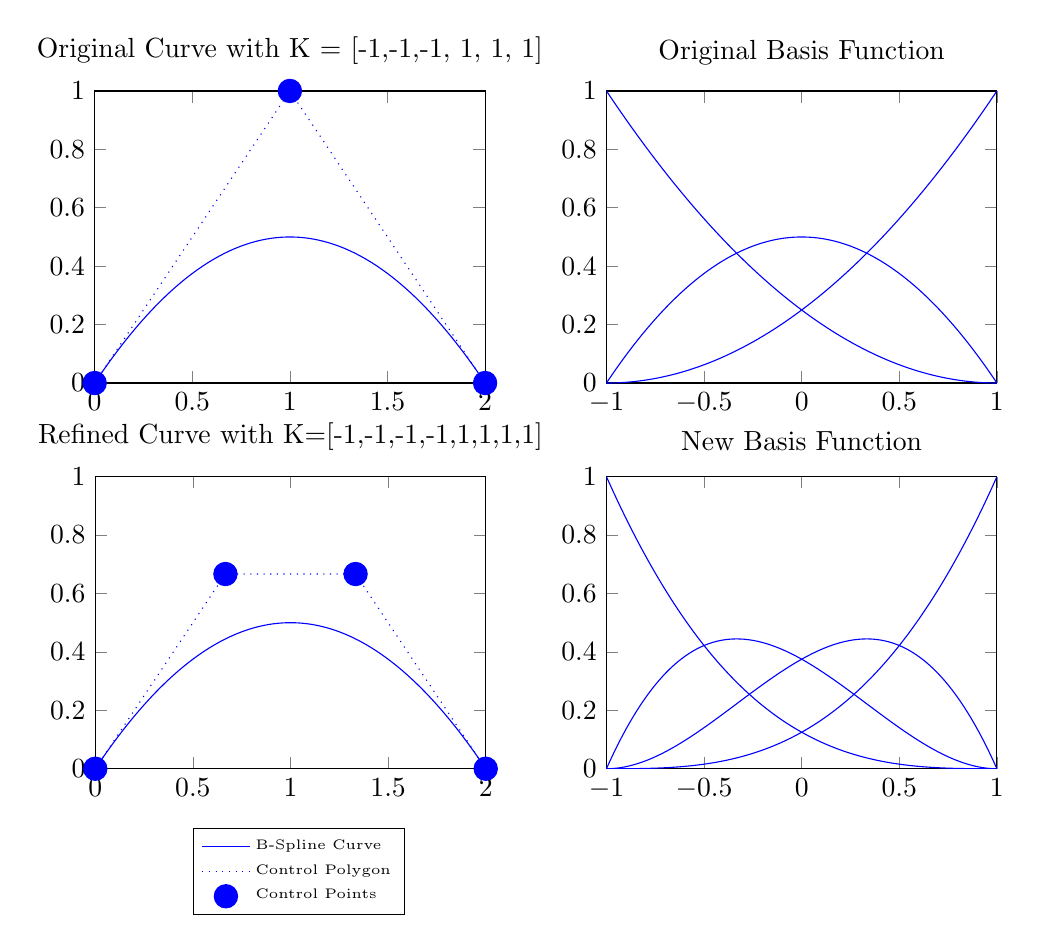
\begin{tikzpicture}[scale=1]

\begin{axis}[%
width=1.95217803030303in,
height=1.46030765503876in,
scale only axis,
xmin=0,
xmax=2,
ymin=0,
ymax=1,
name=plot1,
title={Original  Curve  with  K = [-1,-1,-1, 1, 1, 1]}
]
\addplot [color=blue,solid,forget plot]
  table[row sep=crcr]{
0	0	\\
0.0100502512562815	0.00999974748112426	\\
0.0201005025125628	0.019898487411934	\\
0.0301507537688442	0.0296962197924295	\\
0.0402010050251256	0.0393929446226105	\\
0.050251256281407	0.0489886619024772	\\
0.0603015075376885	0.0584833716320295	\\
0.0703517587939698	0.0678770738112674	\\
0.0804020100502513	0.0771697684401909	\\
0.0904522613065326	0.0863614555188	\\
0.100502512562814	0.0954521350470948	\\
0.110552763819096	0.104441807025075	\\
0.120603015075377	0.113330471452741	\\
0.130653266331658	0.122118128330093	\\
0.14070351758794	0.13080477765713	\\
0.150753768844221	0.139390419433853	\\
0.160804020100503	0.147875053660261	\\
0.170854271356784	0.156258680336355	\\
0.180904522613065	0.164541299462135	\\
0.190954773869347	0.1727229110376	\\
0.201005025125628	0.180803515062751	\\
0.21105527638191	0.188783111537587	\\
0.221105527638191	0.19666170046211	\\
0.231155778894472	0.204439281836317	\\
0.241206030150754	0.212115855660211	\\
0.251256281407035	0.21969142193379	\\
0.261306532663317	0.227165980657054	\\
0.271356783919598	0.234539531830004	\\
0.281407035175879	0.24181207545264	\\
0.291457286432161	0.248983611524961	\\
0.301507537688442	0.256054140046968	\\
0.311557788944724	0.263023661018661	\\
0.321608040201005	0.269892174440039	\\
0.331658291457286	0.276659680311103	\\
0.341708542713568	0.283326178631853	\\
0.351758793969849	0.289891669402288	\\
0.361809045226131	0.296356152622409	\\
0.371859296482412	0.302719628292215	\\
0.381909547738693	0.308982096411707	\\
0.391959798994975	0.315143556980884	\\
0.402010050251256	0.321204009999747	\\
0.412060301507538	0.327163455468296	\\
0.422110552763819	0.333021893386531	\\
0.4321608040201	0.338779323754451	\\
0.442211055276382	0.344435746572056	\\
0.452261306532663	0.349991161839347	\\
0.462311557788945	0.355445569556324	\\
0.472361809045226	0.360798969722987	\\
0.482412060301508	0.366051362339335	\\
0.492462311557789	0.371202747405369	\\
0.50251256281407	0.376253124921088	\\
0.512562814070352	0.381202494886493	\\
0.522613065326633	0.386050857301583	\\
0.532663316582915	0.390798212166359	\\
0.542713567839196	0.395444559480821	\\
0.552763819095477	0.399989899244969	\\
0.562814070351759	0.404434231458802	\\
0.57286432160804	0.40877755612232	\\
0.582914572864322	0.413019873235524	\\
0.592964824120603	0.417161182798414	\\
0.603015075376884	0.42120148481099	\\
0.613065326633166	0.425140779273251	\\
0.623115577889447	0.428979066185197	\\
0.633165829145729	0.43271634554683	\\
0.64321608040201	0.436352617358148	\\
0.653266331658292	0.439887881619151	\\
0.663316582914573	0.44332213832984	\\
0.673366834170854	0.446655387490215	\\
0.683417085427136	0.449887629100275	\\
0.693467336683417	0.453018863160021	\\
0.703517587939699	0.456049089669453	\\
0.71356783919598	0.45897830862857	\\
0.723618090452261	0.461806520037373	\\
0.733668341708543	0.464533723895861	\\
0.743718592964824	0.467159920204035	\\
0.753768844221106	0.469685108961895	\\
0.763819095477387	0.47210929016944	\\
0.773869346733668	0.474432463826671	\\
0.78391959798995	0.476654629933588	\\
0.793969849246231	0.47877578849019	\\
0.804020100502513	0.480795939496477	\\
0.814070351758794	0.482715082952451	\\
0.824120603015075	0.48453321885811	\\
0.834170854271357	0.486250347213454	\\
0.844221105527638	0.487866468018484	\\
0.85427135678392	0.4893815812732	\\
0.864321608040201	0.490795686977602	\\
0.874371859296482	0.492108785131689	\\
0.884422110552764	0.493320875735461	\\
0.894472361809045	0.494431958788919	\\
0.904522613065327	0.495442034292063	\\
0.914572864321608	0.496351102244893	\\
0.924623115577889	0.497159162647408	\\
0.934673366834171	0.497866215499609	\\
0.944723618090452	0.498472260801495	\\
0.954773869346734	0.498977298553067	\\
0.964824120603015	0.499381328754324	\\
0.974874371859296	0.499684351405268	\\
0.984924623115578	0.499886366505896	\\
0.994974874371859	0.499987374056211	\\
1.00502512562814	0.499987374056211	\\
1.01507537688442	0.499886366505896	\\
1.0251256281407	0.499684351405268	\\
1.03517587939699	0.499381328754324	\\
1.04522613065327	0.498977298553067	\\
1.05527638190955	0.498472260801495	\\
1.06532663316583	0.497866215499609	\\
1.07537688442211	0.497159162647408	\\
1.08542713567839	0.496351102244893	\\
1.09547738693467	0.495442034292063	\\
1.10552763819095	0.494431958788919	\\
1.11557788944724	0.493320875735461	\\
1.12562814070352	0.492108785131689	\\
1.1356783919598	0.490795686977602	\\
1.14572864321608	0.4893815812732	\\
1.15577889447236	0.487866468018484	\\
1.16582914572864	0.486250347213454	\\
1.17587939698492	0.48453321885811	\\
1.18592964824121	0.482715082952451	\\
1.19597989949749	0.480795939496477	\\
1.20603015075377	0.47877578849019	\\
1.21608040201005	0.476654629933588	\\
1.22613065326633	0.474432463826671	\\
1.23618090452261	0.47210929016944	\\
1.24623115577889	0.469685108961895	\\
1.25628140703518	0.467159920204035	\\
1.26633165829146	0.464533723895861	\\
1.27638190954774	0.461806520037373	\\
1.28643216080402	0.45897830862857	\\
1.2964824120603	0.456049089669453	\\
1.30653266331658	0.453018863160021	\\
1.31658291457286	0.449887629100275	\\
1.32663316582915	0.446655387490215	\\
1.33668341708543	0.44332213832984	\\
1.34673366834171	0.439887881619151	\\
1.35678391959799	0.436352617358148	\\
1.36683417085427	0.43271634554683	\\
1.37688442211055	0.428979066185197	\\
1.38693467336683	0.425140779273251	\\
1.39698492462312	0.42120148481099	\\
1.4070351758794	0.417161182798414	\\
1.41708542713568	0.413019873235524	\\
1.42713567839196	0.40877755612232	\\
1.43718592964824	0.404434231458802	\\
1.44723618090452	0.399989899244969	\\
1.4572864321608	0.395444559480821	\\
1.46733668341709	0.390798212166359	\\
1.47738693467337	0.386050857301583	\\
1.48743718592965	0.381202494886493	\\
1.49748743718593	0.376253124921088	\\
1.50753768844221	0.371202747405369	\\
1.51758793969849	0.366051362339335	\\
1.52763819095477	0.360798969722987	\\
1.53768844221106	0.355445569556324	\\
1.54773869346734	0.349991161839347	\\
1.55778894472362	0.344435746572056	\\
1.5678391959799	0.338779323754451	\\
1.57788944723618	0.333021893386531	\\
1.58793969849246	0.327163455468296	\\
1.59798994974874	0.321204009999747	\\
1.60804020100503	0.315143556980884	\\
1.61809045226131	0.308982096411707	\\
1.62814070351759	0.302719628292215	\\
1.63819095477387	0.296356152622409	\\
1.64824120603015	0.289891669402288	\\
1.65829145728643	0.283326178631853	\\
1.66834170854271	0.276659680311103	\\
1.67839195979899	0.269892174440039	\\
1.68844221105528	0.263023661018661	\\
1.69849246231156	0.256054140046968	\\
1.70854271356784	0.248983611524961	\\
1.71859296482412	0.24181207545264	\\
1.7286432160804	0.234539531830004	\\
1.73869346733668	0.227165980657054	\\
1.74874371859296	0.21969142193379	\\
1.75879396984925	0.212115855660211	\\
1.76884422110553	0.204439281836317	\\
1.77889447236181	0.19666170046211	\\
1.78894472361809	0.188783111537587	\\
1.79899497487437	0.180803515062751	\\
1.80904522613065	0.1727229110376	\\
1.81909547738693	0.164541299462135	\\
1.82914572864322	0.156258680336355	\\
1.8391959798995	0.147875053660261	\\
1.84924623115578	0.139390419433853	\\
1.85929648241206	0.13080477765713	\\
1.86934673366834	0.122118128330093	\\
1.87939698492462	0.113330471452741	\\
1.8894472361809	0.104441807025075	\\
1.89949748743719	0.0954521350470948	\\
1.90954773869347	0.0863614555188	\\
1.91959798994975	0.0771697684401908	\\
1.92964824120603	0.0678770738112675	\\
1.93969849246231	0.0584833716320295	\\
1.94974874371859	0.0489886619024772	\\
1.95979899497487	0.0393929446226105	\\
1.96984924623116	0.0296962197924294	\\
1.97989949748744	0.0198984874119341	\\
1.98994974874372	0.00999974748112426	\\
2	0	\\
};
\addplot [color=blue,dotted,forget plot]
  table[row sep=crcr]{
0	0	\\
1	1	\\
2	0	\\
};
\addplot [color=blue,mark size=4.2pt,only marks,mark=*,mark options={solid},forget plot]
  table[row sep=crcr]{
0	0	\\
1	1	\\
2	0	\\
};
\end{axis}

\begin{axis}[%
width=1.95217803030303in,
height=1.46030765503876in,
scale only axis,
xmin=-1,
xmax=1,
ymin=0,
ymax=1,
name=plot2,
at=(plot1.right of south east),
anchor=left of south west,
title={Original Basis Function}
]
\addplot [color=blue,solid,forget plot]
  table[row sep=crcr]{
-1	1	\\
-0.989949748743719	0.989975000631297	\\
-0.979899497487437	0.980000505037751	\\
-0.969849246231156	0.970076513219363	\\
-0.959798994974874	0.960203025176132	\\
-0.949748743718593	0.950380040908058	\\
-0.939698492462312	0.940607560415141	\\
-0.92964824120603	0.930885583697381	\\
-0.919597989949749	0.921214110754779	\\
-0.909547738693467	0.911593141587334	\\
-0.899497487437186	0.902022676195046	\\
-0.889447236180904	0.892502714577915	\\
-0.879396984924623	0.883033256735941	\\
-0.869346733668342	0.873614302669125	\\
-0.85929648241206	0.864245852377465	\\
-0.849246231155779	0.854927905860963	\\
-0.839195979899497	0.845660463119618	\\
-0.829145728643216	0.83644352415343	\\
-0.819095477386935	0.8272770889624	\\
-0.809045226130653	0.818161157546527	\\
-0.798994974874372	0.80909572990581	\\
-0.78894472361809	0.800080806040251	\\
-0.778894472361809	0.79111638594985	\\
-0.768844221105528	0.782202469634605	\\
-0.758793969849246	0.773339057094518	\\
-0.748743718592965	0.764526148329588	\\
-0.738693467336683	0.755763743339815	\\
-0.728643216080402	0.747051842125199	\\
-0.718592964824121	0.73839044468574	\\
-0.708542713567839	0.729779551021439	\\
-0.698492462311558	0.721219161132295	\\
-0.688442211055276	0.712709275018308	\\
-0.678391959798995	0.704249892679478	\\
-0.668341708542714	0.695841014115805	\\
-0.658291457286432	0.68748263932729	\\
-0.648241206030151	0.679174768313932	\\
-0.638190954773869	0.67091740107573	\\
-0.628140703517588	0.662710537612687	\\
-0.618090452261307	0.6545541779248	\\
-0.608040201005025	0.64644832201207	\\
-0.597989949748744	0.638392969874498	\\
-0.587939698492462	0.630388121512083	\\
-0.577889447236181	0.622433776924825	\\
-0.5678391959799	0.614529936112725	\\
-0.557788944723618	0.606676599075781	\\
-0.547738693467337	0.598873765813995	\\
-0.537688442211055	0.591121436327365	\\
-0.527638190954774	0.583419610615894	\\
-0.517587939698492	0.575768288679579	\\
-0.507537688442211	0.568167470518421	\\
-0.49748743718593	0.560617156132421	\\
-0.487437185929648	0.553117345521578	\\
-0.477386934673367	0.545668038685892	\\
-0.467336683417085	0.538269235625363	\\
-0.457286432160804	0.530920936339991	\\
-0.447236180904523	0.523623140829777	\\
-0.437185929648241	0.51637584909472	\\
-0.42713567839196	0.50917906113482	\\
-0.417085427135678	0.502032776950077	\\
-0.407035175879397	0.494936996540491	\\
-0.396984924623116	0.487891719906063	\\
-0.386934673366834	0.480896947046792	\\
-0.376884422110553	0.473952677962678	\\
-0.366834170854271	0.467058912653721	\\
-0.35678391959799	0.460215651119921	\\
-0.346733668341708	0.453422893361279	\\
-0.336683417085427	0.446680639377794	\\
-0.326633165829146	0.439988889169465	\\
-0.316582914572864	0.433347642736295	\\
-0.306532663316583	0.426756900078281	\\
-0.296482412060301	0.420216661195424	\\
-0.28643216080402	0.413726926087725	\\
-0.276381909547739	0.407287694755183	\\
-0.266331658291457	0.400898967197798	\\
-0.256281407035176	0.39456074341557	\\
-0.246231155778894	0.3882730234085	\\
-0.236180904522613	0.382035807176586	\\
-0.226130653266332	0.37584909471983	\\
-0.21608040201005	0.369712886038231	\\
-0.206030150753769	0.36362718113179	\\
-0.195979899497487	0.357591980000505	\\
-0.185929648241206	0.351607282644378	\\
-0.175879396984925	0.345673089063407	\\
-0.165829145728643	0.339789399257595	\\
-0.155778894472362	0.333956213226939	\\
-0.14572864321608	0.32817353097144	\\
-0.135678391959799	0.322441352491099	\\
-0.125628140703518	0.316759677785915	\\
-0.115577889447236	0.311128506855887	\\
-0.105527638190955	0.305547839701018	\\
-0.0954773869346733	0.300017676321305	\\
-0.085427135678392	0.29453801671675	\\
-0.0753768844221105	0.289108860887351	\\
-0.0653266331658291	0.28373020883311	\\
-0.0552763819095478	0.278402060554026	\\
-0.0452261306532663	0.2731244160501	\\
-0.035175879396985	0.26789727532133	\\
-0.0251256281407035	0.262720638367718	\\
-0.0150753768844221	0.257594505189263	\\
-0.00502512562814073	0.252518875785965	\\
0.00502512562814061	0.247493750157824	\\
0.0150753768844221	0.242519128304841	\\
0.0251256281407035	0.237595010227014	\\
0.035175879396985	0.232721395924345	\\
0.0452261306532664	0.227898285396833	\\
0.0552763819095476	0.223125678644479	\\
0.0653266331658291	0.218403575667281	\\
0.0753768844221105	0.213731976465241	\\
0.085427135678392	0.209110881038358	\\
0.0954773869346734	0.204540289386632	\\
0.105527638190955	0.200020201510063	\\
0.115577889447236	0.195550617408651	\\
0.125628140703518	0.191131537082397	\\
0.135678391959799	0.1867629605313	\\
0.14572864321608	0.18244488775536	\\
0.155778894472362	0.178177318754577	\\
0.165829145728643	0.173960253528951	\\
0.175879396984925	0.169793692078483	\\
0.185929648241206	0.165677634403172	\\
0.195979899497488	0.161612080503018	\\
0.206030150753769	0.157597030378021	\\
0.21608040201005	0.153632484028181	\\
0.226130653266332	0.149718441453499	\\
0.236180904522613	0.145854902653973	\\
0.246231155778895	0.142041867629605	\\
0.256281407035176	0.138279336380394	\\
0.266331658291457	0.134567308906341	\\
0.276381909547739	0.130905785207444	\\
0.28643216080402	0.127294765283705	\\
0.296482412060302	0.123734249135123	\\
0.306532663316583	0.120224236761698	\\
0.316582914572864	0.11676472816343	\\
0.326633165829146	0.11335572334032	\\
0.336683417085427	0.109997222292366	\\
0.346733668341709	0.10668922501957	\\
0.35678391959799	0.103431731521931	\\
0.366834170854271	0.10022474179945	\\
0.376884422110553	0.097068255852125	\\
0.386934673366834	0.0939622736799576	\\
0.396984924623116	0.0909067952829474	\\
0.407035175879397	0.0879018206610944	\\
0.417085427135678	0.0849473498143987	\\
0.42713567839196	0.08204338274286	\\
0.437185929648241	0.0791899194464786	\\
0.447236180904523	0.0763869599252544	\\
0.457286432160804	0.0736345041791874	\\
0.467336683417085	0.0709325522082776	\\
0.477386934673367	0.0682811040125249	\\
0.487437185929648	0.0656801595919295	\\
0.49748743718593	0.0631297189464912	\\
0.507537688442211	0.0606297820762102	\\
0.517587939698492	0.0581803489810864	\\
0.527638190954774	0.0557814196611197	\\
0.537688442211055	0.0534329941163102	\\
0.547738693467337	0.0511350723466579	\\
0.557788944723618	0.0488876543521628	\\
0.567839195979899	0.0466907401328249	\\
0.577889447236181	0.0445443296886442	\\
0.587939698492462	0.0424484230196207	\\
0.597989949748744	0.0404030201257544	\\
0.608040201005025	0.0384081210070453	\\
0.618090452261306	0.0364637256634934	\\
0.628140703517588	0.0345698340950986	\\
0.638190954773869	0.0327264463018611	\\
0.648241206030151	0.0309335622837807	\\
0.658291457286432	0.0291911820408575	\\
0.668341708542713	0.0274993055730916	\\
0.678391959798995	0.0258579328804828	\\
0.688442211055276	0.0242670639630312	\\
0.698492462311558	0.0227266988207368	\\
0.708542713567839	0.0212368374535996	\\
0.71859296482412	0.0197974798616197	\\
0.728643216080402	0.0184086260447969	\\
0.738693467336683	0.0170702760031312	\\
0.748743718592965	0.0157824297366228	\\
0.758793969849246	0.0145450872452716	\\
0.768844221105528	0.0133582485290775	\\
0.778894472361809	0.0122219135880407	\\
0.78894472361809	0.0111360824221611	\\
0.798994974874372	0.0101007550314386	\\
0.809045226130653	0.00911593141587333	\\
0.819095477386935	0.00818161157546526	\\
0.829145728643216	0.0072977955102144	\\
0.839195979899497	0.00646448322012071	\\
0.849246231155779	0.00568167470518421	\\
0.85929648241206	0.00494936996540491	\\
0.869346733668342	0.0042675690007828	\\
0.879396984924623	0.0036362718113179	\\
0.889447236180904	0.00305547839701018	\\
0.899497487437186	0.00252518875785965	\\
0.909547738693467	0.00204540289386631	\\
0.919597989949749	0.00161612080503017	\\
0.92964824120603	0.00123734249135123	\\
0.939698492462312	0.000909067952829475	\\
0.949748743718593	0.000631297189464912	\\
0.959798994974874	0.000404030201257543	\\
0.969849246231156	0.000227266988207367	\\
0.979899497487437	0.000101007550314387	\\
0.989949748743719	2.52518875785967e-05	\\
1	0	\\
};
\addplot [color=blue,solid,forget plot]
  table[row sep=crcr]{
-1	0	\\
-0.989949748743719	0.00999974748112426	\\
-0.979899497487437	0.019898487411934	\\
-0.969849246231156	0.0296962197924295	\\
-0.959798994974874	0.0393929446226105	\\
-0.949748743718593	0.0489886619024772	\\
-0.939698492462312	0.0584833716320295	\\
-0.92964824120603	0.0678770738112674	\\
-0.919597989949749	0.0771697684401909	\\
-0.909547738693467	0.0863614555188	\\
-0.899497487437186	0.0954521350470948	\\
-0.889447236180904	0.104441807025075	\\
-0.879396984924623	0.113330471452741	\\
-0.869346733668342	0.122118128330093	\\
-0.85929648241206	0.13080477765713	\\
-0.849246231155779	0.139390419433853	\\
-0.839195979899497	0.147875053660261	\\
-0.829145728643216	0.156258680336355	\\
-0.819095477386935	0.164541299462135	\\
-0.809045226130653	0.1727229110376	\\
-0.798994974874372	0.180803515062751	\\
-0.78894472361809	0.188783111537587	\\
-0.778894472361809	0.19666170046211	\\
-0.768844221105528	0.204439281836317	\\
-0.758793969849246	0.212115855660211	\\
-0.748743718592965	0.21969142193379	\\
-0.738693467336683	0.227165980657054	\\
-0.728643216080402	0.234539531830004	\\
-0.718592964824121	0.24181207545264	\\
-0.708542713567839	0.248983611524961	\\
-0.698492462311558	0.256054140046968	\\
-0.688442211055276	0.263023661018661	\\
-0.678391959798995	0.269892174440039	\\
-0.668341708542714	0.276659680311103	\\
-0.658291457286432	0.283326178631853	\\
-0.648241206030151	0.289891669402288	\\
-0.638190954773869	0.296356152622409	\\
-0.628140703517588	0.302719628292215	\\
-0.618090452261307	0.308982096411707	\\
-0.608040201005025	0.315143556980884	\\
-0.597989949748744	0.321204009999747	\\
-0.587939698492462	0.327163455468296	\\
-0.577889447236181	0.333021893386531	\\
-0.5678391959799	0.338779323754451	\\
-0.557788944723618	0.344435746572056	\\
-0.547738693467337	0.349991161839347	\\
-0.537688442211055	0.355445569556324	\\
-0.527638190954774	0.360798969722987	\\
-0.517587939698492	0.366051362339335	\\
-0.507537688442211	0.371202747405369	\\
-0.49748743718593	0.376253124921088	\\
-0.487437185929648	0.381202494886493	\\
-0.477386934673367	0.386050857301583	\\
-0.467336683417085	0.390798212166359	\\
-0.457286432160804	0.395444559480821	\\
-0.447236180904523	0.399989899244969	\\
-0.437185929648241	0.404434231458802	\\
-0.42713567839196	0.40877755612232	\\
-0.417085427135678	0.413019873235524	\\
-0.407035175879397	0.417161182798414	\\
-0.396984924623116	0.42120148481099	\\
-0.386934673366834	0.425140779273251	\\
-0.376884422110553	0.428979066185197	\\
-0.366834170854271	0.43271634554683	\\
-0.35678391959799	0.436352617358148	\\
-0.346733668341708	0.439887881619151	\\
-0.336683417085427	0.44332213832984	\\
-0.326633165829146	0.446655387490215	\\
-0.316582914572864	0.449887629100275	\\
-0.306532663316583	0.453018863160021	\\
-0.296482412060301	0.456049089669453	\\
-0.28643216080402	0.45897830862857	\\
-0.276381909547739	0.461806520037373	\\
-0.266331658291457	0.464533723895861	\\
-0.256281407035176	0.467159920204035	\\
-0.246231155778894	0.469685108961895	\\
-0.236180904522613	0.47210929016944	\\
-0.226130653266332	0.474432463826671	\\
-0.21608040201005	0.476654629933588	\\
-0.206030150753769	0.47877578849019	\\
-0.195979899497487	0.480795939496477	\\
-0.185929648241206	0.482715082952451	\\
-0.175879396984925	0.48453321885811	\\
-0.165829145728643	0.486250347213454	\\
-0.155778894472362	0.487866468018484	\\
-0.14572864321608	0.4893815812732	\\
-0.135678391959799	0.490795686977602	\\
-0.125628140703518	0.492108785131689	\\
-0.115577889447236	0.493320875735461	\\
-0.105527638190955	0.494431958788919	\\
-0.0954773869346733	0.495442034292063	\\
-0.085427135678392	0.496351102244893	\\
-0.0753768844221105	0.497159162647408	\\
-0.0653266331658291	0.497866215499609	\\
-0.0552763819095478	0.498472260801495	\\
-0.0452261306532663	0.498977298553067	\\
-0.035175879396985	0.499381328754324	\\
-0.0251256281407035	0.499684351405268	\\
-0.0150753768844221	0.499886366505896	\\
-0.00502512562814073	0.499987374056211	\\
0.00502512562814061	0.499987374056211	\\
0.0150753768844221	0.499886366505896	\\
0.0251256281407035	0.499684351405268	\\
0.035175879396985	0.499381328754324	\\
0.0452261306532664	0.498977298553067	\\
0.0552763819095476	0.498472260801495	\\
0.0653266331658291	0.497866215499609	\\
0.0753768844221105	0.497159162647408	\\
0.085427135678392	0.496351102244893	\\
0.0954773869346734	0.495442034292063	\\
0.105527638190955	0.494431958788919	\\
0.115577889447236	0.493320875735461	\\
0.125628140703518	0.492108785131689	\\
0.135678391959799	0.490795686977602	\\
0.14572864321608	0.4893815812732	\\
0.155778894472362	0.487866468018484	\\
0.165829145728643	0.486250347213454	\\
0.175879396984925	0.48453321885811	\\
0.185929648241206	0.482715082952451	\\
0.195979899497488	0.480795939496477	\\
0.206030150753769	0.47877578849019	\\
0.21608040201005	0.476654629933588	\\
0.226130653266332	0.474432463826671	\\
0.236180904522613	0.47210929016944	\\
0.246231155778895	0.469685108961895	\\
0.256281407035176	0.467159920204035	\\
0.266331658291457	0.464533723895861	\\
0.276381909547739	0.461806520037373	\\
0.28643216080402	0.45897830862857	\\
0.296482412060302	0.456049089669453	\\
0.306532663316583	0.453018863160021	\\
0.316582914572864	0.449887629100275	\\
0.326633165829146	0.446655387490215	\\
0.336683417085427	0.44332213832984	\\
0.346733668341709	0.439887881619151	\\
0.35678391959799	0.436352617358148	\\
0.366834170854271	0.43271634554683	\\
0.376884422110553	0.428979066185197	\\
0.386934673366834	0.425140779273251	\\
0.396984924623116	0.42120148481099	\\
0.407035175879397	0.417161182798414	\\
0.417085427135678	0.413019873235524	\\
0.42713567839196	0.40877755612232	\\
0.437185929648241	0.404434231458802	\\
0.447236180904523	0.399989899244969	\\
0.457286432160804	0.395444559480821	\\
0.467336683417085	0.390798212166359	\\
0.477386934673367	0.386050857301583	\\
0.487437185929648	0.381202494886493	\\
0.49748743718593	0.376253124921088	\\
0.507537688442211	0.371202747405369	\\
0.517587939698492	0.366051362339335	\\
0.527638190954774	0.360798969722987	\\
0.537688442211055	0.355445569556324	\\
0.547738693467337	0.349991161839347	\\
0.557788944723618	0.344435746572056	\\
0.567839195979899	0.338779323754451	\\
0.577889447236181	0.333021893386531	\\
0.587939698492462	0.327163455468296	\\
0.597989949748744	0.321204009999747	\\
0.608040201005025	0.315143556980884	\\
0.618090452261306	0.308982096411707	\\
0.628140703517588	0.302719628292215	\\
0.638190954773869	0.296356152622409	\\
0.648241206030151	0.289891669402288	\\
0.658291457286432	0.283326178631853	\\
0.668341708542713	0.276659680311103	\\
0.678391959798995	0.269892174440039	\\
0.688442211055276	0.263023661018661	\\
0.698492462311558	0.256054140046968	\\
0.708542713567839	0.248983611524961	\\
0.71859296482412	0.24181207545264	\\
0.728643216080402	0.234539531830004	\\
0.738693467336683	0.227165980657054	\\
0.748743718592965	0.21969142193379	\\
0.758793969849246	0.212115855660211	\\
0.768844221105528	0.204439281836317	\\
0.778894472361809	0.19666170046211	\\
0.78894472361809	0.188783111537587	\\
0.798994974874372	0.180803515062751	\\
0.809045226130653	0.1727229110376	\\
0.819095477386935	0.164541299462135	\\
0.829145728643216	0.156258680336355	\\
0.839195979899497	0.147875053660261	\\
0.849246231155779	0.139390419433853	\\
0.85929648241206	0.13080477765713	\\
0.869346733668342	0.122118128330093	\\
0.879396984924623	0.113330471452741	\\
0.889447236180904	0.104441807025075	\\
0.899497487437186	0.0954521350470948	\\
0.909547738693467	0.0863614555188	\\
0.919597989949749	0.0771697684401908	\\
0.92964824120603	0.0678770738112675	\\
0.939698492462312	0.0584833716320295	\\
0.949748743718593	0.0489886619024772	\\
0.959798994974874	0.0393929446226105	\\
0.969849246231156	0.0296962197924294	\\
0.979899497487437	0.0198984874119341	\\
0.989949748743719	0.00999974748112426	\\
1	0	\\
};
\addplot [color=blue,solid,forget plot]
  table[row sep=crcr]{
-1	0	\\
-0.989949748743719	2.52518875785967e-05	\\
-0.979899497487437	0.000101007550314386	\\
-0.969849246231156	0.000227266988207369	\\
-0.959798994974874	0.000404030201257543	\\
-0.949748743718593	0.000631297189464912	\\
-0.939698492462312	0.000909067952829475	\\
-0.92964824120603	0.00123734249135123	\\
-0.919597989949749	0.00161612080503018	\\
-0.909547738693467	0.00204540289386631	\\
-0.899497487437186	0.00252518875785965	\\
-0.889447236180904	0.00305547839701018	\\
-0.879396984924623	0.00363627181131789	\\
-0.869346733668342	0.00426756900078281	\\
-0.85929648241206	0.00494936996540491	\\
-0.849246231155779	0.00568167470518421	\\
-0.839195979899497	0.00646448322012071	\\
-0.829145728643216	0.00729779551021439	\\
-0.819095477386935	0.00818161157546527	\\
-0.809045226130653	0.00911593141587333	\\
-0.798994974874372	0.0101007550314386	\\
-0.78894472361809	0.0111360824221611	\\
-0.778894472361809	0.0122219135880407	\\
-0.768844221105528	0.0133582485290775	\\
-0.758793969849246	0.0145450872452716	\\
-0.748743718592965	0.0157824297366228	\\
-0.738693467336683	0.0170702760031312	\\
-0.728643216080402	0.0184086260447969	\\
-0.718592964824121	0.0197974798616197	\\
-0.708542713567839	0.0212368374535996	\\
-0.698492462311558	0.0227266988207368	\\
-0.688442211055276	0.0242670639630312	\\
-0.678391959798995	0.0258579328804828	\\
-0.668341708542714	0.0274993055730916	\\
-0.658291457286432	0.0291911820408575	\\
-0.648241206030151	0.0309335622837807	\\
-0.638190954773869	0.0327264463018611	\\
-0.628140703517588	0.0345698340950986	\\
-0.618090452261307	0.0364637256634933	\\
-0.608040201005025	0.0384081210070453	\\
-0.597989949748744	0.0404030201257544	\\
-0.587939698492462	0.0424484230196207	\\
-0.577889447236181	0.0445443296886442	\\
-0.5678391959799	0.0466907401328249	\\
-0.557788944723618	0.0488876543521628	\\
-0.547738693467337	0.0511350723466579	\\
-0.537688442211055	0.0534329941163102	\\
-0.527638190954774	0.0557814196611197	\\
-0.517587939698492	0.0581803489810863	\\
-0.507537688442211	0.0606297820762102	\\
-0.49748743718593	0.0631297189464912	\\
-0.487437185929648	0.0656801595919295	\\
-0.477386934673367	0.0682811040125249	\\
-0.467336683417085	0.0709325522082776	\\
-0.457286432160804	0.0736345041791874	\\
-0.447236180904523	0.0763869599252544	\\
-0.437185929648241	0.0791899194464786	\\
-0.42713567839196	0.08204338274286	\\
-0.417085427135678	0.0849473498143986	\\
-0.407035175879397	0.0879018206610944	\\
-0.396984924623116	0.0909067952829474	\\
-0.386934673366834	0.0939622736799576	\\
-0.376884422110553	0.097068255852125	\\
-0.366834170854271	0.10022474179945	\\
-0.35678391959799	0.103431731521931	\\
-0.346733668341708	0.10668922501957	\\
-0.336683417085427	0.109997222292366	\\
-0.326633165829146	0.11335572334032	\\
-0.316582914572864	0.11676472816343	\\
-0.306532663316583	0.120224236761698	\\
-0.296482412060301	0.123734249135123	\\
-0.28643216080402	0.127294765283705	\\
-0.276381909547739	0.130905785207444	\\
-0.266331658291457	0.134567308906341	\\
-0.256281407035176	0.138279336380394	\\
-0.246231155778894	0.142041867629605	\\
-0.236180904522613	0.145854902653973	\\
-0.226130653266332	0.149718441453499	\\
-0.21608040201005	0.153632484028181	\\
-0.206030150753769	0.157597030378021	\\
-0.195979899497487	0.161612080503018	\\
-0.185929648241206	0.165677634403172	\\
-0.175879396984925	0.169793692078483	\\
-0.165829145728643	0.173960253528951	\\
-0.155778894472362	0.178177318754577	\\
-0.14572864321608	0.18244488775536	\\
-0.135678391959799	0.1867629605313	\\
-0.125628140703518	0.191131537082397	\\
-0.115577889447236	0.195550617408651	\\
-0.105527638190955	0.200020201510063	\\
-0.0954773869346733	0.204540289386632	\\
-0.085427135678392	0.209110881038358	\\
-0.0753768844221105	0.213731976465241	\\
-0.0653266331658291	0.218403575667281	\\
-0.0552763819095478	0.223125678644479	\\
-0.0452261306532663	0.227898285396833	\\
-0.035175879396985	0.232721395924345	\\
-0.0251256281407035	0.237595010227014	\\
-0.0150753768844221	0.242519128304841	\\
-0.00502512562814073	0.247493750157824	\\
0.00502512562814061	0.252518875785965	\\
0.0150753768844221	0.257594505189263	\\
0.0251256281407035	0.262720638367718	\\
0.035175879396985	0.26789727532133	\\
0.0452261306532664	0.2731244160501	\\
0.0552763819095476	0.278402060554026	\\
0.0653266331658291	0.28373020883311	\\
0.0753768844221105	0.289108860887351	\\
0.085427135678392	0.29453801671675	\\
0.0954773869346734	0.300017676321305	\\
0.105527638190955	0.305547839701018	\\
0.115577889447236	0.311128506855887	\\
0.125628140703518	0.316759677785915	\\
0.135678391959799	0.322441352491099	\\
0.14572864321608	0.32817353097144	\\
0.155778894472362	0.333956213226939	\\
0.165829145728643	0.339789399257594	\\
0.175879396984925	0.345673089063407	\\
0.185929648241206	0.351607282644378	\\
0.195979899497488	0.357591980000505	\\
0.206030150753769	0.36362718113179	\\
0.21608040201005	0.369712886038231	\\
0.226130653266332	0.37584909471983	\\
0.236180904522613	0.382035807176586	\\
0.246231155778895	0.3882730234085	\\
0.256281407035176	0.39456074341557	\\
0.266331658291457	0.400898967197798	\\
0.276381909547739	0.407287694755183	\\
0.28643216080402	0.413726926087725	\\
0.296482412060302	0.420216661195424	\\
0.306532663316583	0.426756900078281	\\
0.316582914572864	0.433347642736295	\\
0.326633165829146	0.439988889169465	\\
0.336683417085427	0.446680639377794	\\
0.346733668341709	0.453422893361279	\\
0.35678391959799	0.460215651119921	\\
0.366834170854271	0.467058912653721	\\
0.376884422110553	0.473952677962678	\\
0.386934673366834	0.480896947046792	\\
0.396984924623116	0.487891719906063	\\
0.407035175879397	0.494936996540491	\\
0.417085427135678	0.502032776950077	\\
0.42713567839196	0.50917906113482	\\
0.437185929648241	0.51637584909472	\\
0.447236180904523	0.523623140829777	\\
0.457286432160804	0.530920936339991	\\
0.467336683417085	0.538269235625363	\\
0.477386934673367	0.545668038685892	\\
0.487437185929648	0.553117345521578	\\
0.49748743718593	0.560617156132421	\\
0.507537688442211	0.568167470518421	\\
0.517587939698492	0.575768288679579	\\
0.527638190954774	0.583419610615894	\\
0.537688442211055	0.591121436327365	\\
0.547738693467337	0.598873765813995	\\
0.557788944723618	0.606676599075781	\\
0.567839195979899	0.614529936112724	\\
0.577889447236181	0.622433776924825	\\
0.587939698492462	0.630388121512083	\\
0.597989949748744	0.638392969874498	\\
0.608040201005025	0.64644832201207	\\
0.618090452261306	0.6545541779248	\\
0.628140703517588	0.662710537612687	\\
0.638190954773869	0.67091740107573	\\
0.648241206030151	0.679174768313932	\\
0.658291457286432	0.68748263932729	\\
0.668341708542713	0.695841014115805	\\
0.678391959798995	0.704249892679478	\\
0.688442211055276	0.712709275018308	\\
0.698492462311558	0.721219161132295	\\
0.708542713567839	0.729779551021439	\\
0.71859296482412	0.73839044468574	\\
0.728643216080402	0.747051842125199	\\
0.738693467336683	0.755763743339815	\\
0.748743718592965	0.764526148329588	\\
0.758793969849246	0.773339057094518	\\
0.768844221105528	0.782202469634605	\\
0.778894472361809	0.79111638594985	\\
0.78894472361809	0.800080806040251	\\
0.798994974874372	0.80909572990581	\\
0.809045226130653	0.818161157546527	\\
0.819095477386935	0.8272770889624	\\
0.829145728643216	0.83644352415343	\\
0.839195979899497	0.845660463119618	\\
0.849246231155779	0.854927905860963	\\
0.85929648241206	0.864245852377465	\\
0.869346733668342	0.873614302669125	\\
0.879396984924623	0.883033256735941	\\
0.889447236180904	0.892502714577915	\\
0.899497487437186	0.902022676195046	\\
0.909547738693467	0.911593141587334	\\
0.919597989949749	0.921214110754779	\\
0.92964824120603	0.930885583697381	\\
0.939698492462312	0.940607560415141	\\
0.949748743718593	0.950380040908058	\\
0.959798994974874	0.960203025176132	\\
0.969849246231156	0.970076513219363	\\
0.979899497487437	0.980000505037751	\\
0.989949748743719	0.989975000631297	\\
1	1	\\
};
\end{axis}

\begin{axis}[%
width=1.95217803030303in,
height=1.46030765503876in,
scale only axis,
xmin=-1,
xmax=1,
ymin=0,
ymax=1,
name=plot4,
at=(plot2.below south west),
anchor=above north west,
title={New Basis Function}
]
\addplot [color=blue,solid,forget plot]
  table[row sep=crcr]{
-1	1	\\
-0.989949748743719	0.985000251884406	\\
-0.979899497487437	0.970151253730839	\\
-0.969849246231156	0.955452244175855	\\
-0.959798994974874	0.940902461856009	\\
-0.949748743718593	0.926501145407855	\\
-0.939698492462312	0.912247533467951	\\
-0.92964824120603	0.89814086467285	\\
-0.919597989949749	0.88418037765911	\\
-0.909547738693467	0.870365311063284	\\
-0.899497487437186	0.856694903521928	\\
-0.889447236180904	0.843168393671598	\\
-0.879396984924623	0.829785020148849	\\
-0.869346733668342	0.816544021590237	\\
-0.85929648241206	0.803444636632317	\\
-0.849246231155779	0.790486103911644	\\
-0.839195979899497	0.777667662064774	\\
-0.829145728643216	0.764988549728263	\\
-0.819095477386935	0.752448005538665	\\
-0.809045226130653	0.740045268132537	\\
-0.798994974874372	0.727779576146433	\\
-0.78894472361809	0.715650168216908	\\
-0.778894472361809	0.70365628298052	\\
-0.768844221105528	0.691797159073822	\\
-0.758793969849246	0.68007203513337	\\
-0.748743718592965	0.66848014979572	\\
-0.738693467336683	0.657020741697427	\\
-0.728643216080402	0.645693049475046	\\
-0.718592964824121	0.634496311765134	\\
-0.708542713567839	0.623429767204244	\\
-0.698492462311558	0.612492654428934	\\
-0.688442211055276	0.601684212075757	\\
-0.678391959798995	0.59100367878127	\\
-0.668341708542714	0.580450293182029	\\
-0.658291457286432	0.570023293914587	\\
-0.648241206030151	0.559721919615501	\\
-0.638190954773869	0.549545408921327	\\
-0.628140703517588	0.539493000468619	\\
-0.618090452261307	0.529563932893934	\\
-0.608040201005025	0.519757444833826	\\
-0.597989949748744	0.51007277492485	\\
-0.587939698492462	0.500509161803563	\\
-0.577889447236181	0.49106584410652	\\
-0.5678391959799	0.481742060470277	\\
-0.557788944723618	0.472537049531387	\\
-0.547738693467337	0.463450049926408	\\
-0.537688442211055	0.454480300291894	\\
-0.527638190954774	0.445627039264401	\\
-0.517587939698492	0.436889505480485	\\
-0.507537688442211	0.428266937576699	\\
-0.49748743718593	0.419758574189602	\\
-0.487437185929648	0.411363653955746	\\
-0.477386934673367	0.403081415511689	\\
-0.467336683417085	0.394911097493985	\\
-0.457286432160804	0.38685193853919	\\
-0.447236180904523	0.378903177283859	\\
-0.437185929648241	0.371064052364547	\\
-0.42713567839196	0.363333802417811	\\
-0.417085427135678	0.355711666080205	\\
-0.407035175879397	0.348196881988285	\\
-0.396984924623116	0.340788688778607	\\
-0.386934673366834	0.333486325087725	\\
-0.376884422110553	0.326289029552195	\\
-0.366834170854271	0.319196040808573	\\
-0.35678391959799	0.312206597493414	\\
-0.346733668341708	0.305319938243273	\\
-0.336683417085427	0.298535301694706	\\
-0.326633165829146	0.291851926484269	\\
-0.316582914572864	0.285269051248516	\\
-0.306532663316583	0.278785914624002	\\
-0.296482412060301	0.272401755247285	\\
-0.28643216080402	0.266115811754919	\\
-0.276381909547739	0.259927322783458	\\
-0.266331658291457	0.25383552696946	\\
-0.256281407035176	0.247839662949479	\\
-0.246231155778894	0.24193896936007	\\
-0.236180904522613	0.23613268483779	\\
-0.226130653266332	0.230420048019192	\\
-0.21608040201005	0.224800297540834	\\
-0.206030150753769	0.21927267203927	\\
-0.195979899497487	0.213836410151056	\\
-0.185929648241206	0.208490750512747	\\
-0.175879396984925	0.203234931760898	\\
-0.165829145728643	0.198068192532065	\\
-0.155778894472362	0.192989771462804	\\
-0.14572864321608	0.187998907189669	\\
-0.135678391959799	0.183094838349217	\\
-0.125628140703518	0.178276803578002	\\
-0.115577889447236	0.17354404151258	\\
-0.105527638190955	0.168895790789507	\\
-0.0954773869346733	0.164331290045338	\\
-0.085427135678392	0.159849777916628	\\
-0.0753768844221105	0.155450493039933	\\
-0.0653266331658291	0.151132674051807	\\
-0.0552763819095478	0.146895559588808	\\
-0.0452261306532663	0.142738388287489	\\
-0.035175879396985	0.138660398784407	\\
-0.0251256281407035	0.134660829716117	\\
-0.0150753768844221	0.130738919719174	\\
-0.00502512562814073	0.126893907430133	\\
0.00502512562814061	0.123125031485551	\\
0.0150753768844221	0.119431530521982	\\
0.0251256281407035	0.115812643175982	\\
0.035175879396985	0.112267608084106	\\
0.0452261306532664	0.10879566388291	\\
0.0552763819095476	0.10539604920895	\\
0.0653266331658291	0.10206800269878	\\
0.0753768844221105	0.0988107629889555	\\
0.085427135678392	0.0956235687160329	\\
0.0954773869346734	0.092505658516567	\\
0.105527638190955	0.0894562710271136	\\
0.115577889447236	0.0864746448842277	\\
0.125628140703518	0.083560018724465	\\
0.135678391959799	0.0807116311843808	\\
0.14572864321608	0.0779287209005305	\\
0.155778894472362	0.0752105265094697	\\
0.165829145728643	0.0725562866477536	\\
0.175879396984925	0.0699652399519377	\\
0.185929648241206	0.0674366250585774	\\
0.195979899497488	0.0649696806042282	\\
0.206030150753769	0.0625636452254455	\\
0.21608040201005	0.0602177575587846	\\
0.226130653266332	0.057931256240801	\\
0.236180904522613	0.0557033799080501	\\
0.246231155778895	0.0535333671970874	\\
0.256281407035176	0.0514204567444683	\\
0.266331658291457	0.0493638871867481	\\
0.276381909547739	0.0473628971604823	\\
0.28643216080402	0.0454167253022264	\\
0.296482412060302	0.0435246102485357	\\
0.306532663316583	0.0416857906359656	\\
0.316582914572864	0.0398995051010716	\\
0.326633165829146	0.0381649922804091	\\
0.336683417085427	0.0364814908105336	\\
0.346733668341709	0.0348482393280003	\\
0.35678391959799	0.0332644764693648	\\
0.366834170854271	0.0317294408711825	\\
0.376884422110553	0.0302423711700088	\\
0.386934673366834	0.0288025060023991	\\
0.396984924623116	0.0274090840049088	\\
0.407035175879397	0.0260613438140933	\\
0.417085427135678	0.0247585240665082	\\
0.42713567839196	0.0234998633987087	\\
0.437185929648241	0.0222846004472503	\\
0.447236180904523	0.0211119738486884	\\
0.457286432160804	0.0199812222395785	\\
0.467336683417085	0.0188915842564759	\\
0.477386934673367	0.0178422985359362	\\
0.487437185929648	0.0168326037145146	\\
0.49748743718593	0.0158617384287666	\\
0.507537688442211	0.0149289413152477	\\
0.517587939698492	0.0140334510105133	\\
0.527638190954774	0.0131745061511187	\\
0.537688442211055	0.0123513453736194	\\
0.547738693467337	0.0115632073145709	\\
0.557788944723618	0.0108093306105285	\\
0.567839195979899	0.0100889538980476	\\
0.577889447236181	0.00940131581368371	\\
0.587939698492462	0.00874565499399221	\\
0.597989949748744	0.00812121007552852	\\
0.608040201005025	0.00752721969484807	\\
0.618090452261306	0.00696292248850627	\\
0.628140703517588	0.00642755709305854	\\
0.638190954773869	0.00592036214506029	\\
0.648241206030151	0.00544057628106696	\\
0.658291457286432	0.00498743813763395	\\
0.668341708542713	0.0045601863513167	\\
0.678391959798995	0.00415805955867061	\\
0.688442211055276	0.0037802963962511	\\
0.698492462311558	0.00342613550061359	\\
0.708542713567839	0.00309481550831352	\\
0.71859296482412	0.00278557505590629	\\
0.728643216080402	0.00249765277994731	\\
0.738693467336683	0.00223028731699202	\\
0.748743718592965	0.00198271730359583	\\
0.758793969849246	0.00175418137631416	\\
0.768844221105528	0.00154391817170243	\\
0.778894472361809	0.00135116632631606	\\
0.78894472361809	0.00117516447671046	\\
0.798994974874372	0.00101515125944106	\\
0.809045226130653	0.000870365311063283	\\
0.819095477386935	0.000740045268132535	\\
0.829145728643216	0.000623429767204245	\\
0.839195979899497	0.000519757444833826	\\
0.849246231155779	0.000428266937576699	\\
0.85929648241206	0.000348196881988285	\\
0.869346733668342	0.000278785914624002	\\
0.879396984924623	0.000219272672039271	\\
0.889447236180904	0.000168895790789507	\\
0.899497487437186	0.000126893907430133	\\
0.909547738693467	9.25056585165669e-05	\\
0.919597989949749	6.49696806042279e-05	\\
0.92964824120603	4.35246102485358e-05	\\
0.939698492462312	2.74090840049088e-05	\\
0.949748743718593	1.58617384287666e-05	\\
0.959798994974874	8.12121007552849e-06	\\
0.969849246231156	3.42613550061356e-06	\\
0.979899497487437	1.01515125944108e-06	\\
0.989949748743719	1.26893907430135e-07	\\
1	0	\\
};
\addplot [color=blue,solid,forget plot]
  table[row sep=crcr]{
-1	0	\\
-0.989949748743719	0.0149242462406729	\\
-0.979899497487437	0.0295477539207362	\\
-0.969849246231156	0.043872807130524	\\
-0.959798994974874	0.0579016899603697	\\
-0.949748743718593	0.0716366865006074	\\
-0.939698492462312	0.0850800808415706	\\
-0.92964824120603	0.098234157073593	\\
-0.919597989949749	0.111101199287009	\\
-0.909547738693467	0.123683491572151	\\
-0.899497487437186	0.135983318019354	\\
-0.889447236180904	0.148002962718951	\\
-0.879396984924623	0.159744709761276	\\
-0.869346733668342	0.171210843236663	\\
-0.85929648241206	0.182403647235445	\\
-0.849246231155779	0.193325405847956	\\
-0.839195979899497	0.203978403164531	\\
-0.829145728643216	0.214364923275502	\\
-0.819095477386935	0.224487250271204	\\
-0.809045226130653	0.23434766824197	\\
-0.798994974874372	0.243948461278134	\\
-0.78894472361809	0.253291913470029	\\
-0.778894472361809	0.26238030890799	\\
-0.768844221105528	0.271215931682351	\\
-0.758793969849246	0.279801065883444	\\
-0.748743718592965	0.288137995601603	\\
-0.738693467336683	0.296229004927164	\\
-0.728643216080402	0.304076377950458	\\
-0.718592964824121	0.31168239876182	\\
-0.708542713567839	0.319049351451584	\\
-0.698492462311558	0.326179520110083	\\
-0.688442211055276	0.333075188827651	\\
-0.678391959798995	0.339738641694622	\\
-0.668341708542714	0.34617216280133	\\
-0.658291457286432	0.352378036238108	\\
-0.648241206030151	0.35835854609529	\\
-0.638190954773869	0.36411597646321	\\
-0.628140703517588	0.369652611432202	\\
-0.618090452261307	0.374970735092599	\\
-0.608040201005025	0.380072631534735	\\
-0.597989949748744	0.384960584848944	\\
-0.587939698492462	0.389636879125559	\\
-0.577889447236181	0.394103798454914	\\
-0.5678391959799	0.398363626927344	\\
-0.557788944723618	0.402418648633181	\\
-0.547738693467337	0.40627114766276	\\
-0.537688442211055	0.409923408106414	\\
-0.527638190954774	0.413377714054477	\\
-0.517587939698492	0.416636349597283	\\
-0.507537688442211	0.419701598825165	\\
-0.49748743718593	0.422575745828458	\\
-0.487437185929648	0.425261074697494	\\
-0.477386934673367	0.427759869522609	\\
-0.467336683417085	0.430074414394134	\\
-0.457286432160804	0.432206993402405	\\
-0.447236180904523	0.434159890637755	\\
-0.437185929648241	0.435935390190517	\\
-0.42713567839196	0.437535776151026	\\
-0.417085427135678	0.438963332609615	\\
-0.407035175879397	0.440220343656618	\\
-0.396984924623116	0.441309093382369	\\
-0.386934673366834	0.4422318658772	\\
-0.376884422110553	0.442990945231448	\\
-0.366834170854271	0.443588615535443	\\
-0.35678391959799	0.444027160879522	\\
-0.346733668341708	0.444308865354017	\\
-0.336683417085427	0.444436013049262	\\
-0.326633165829146	0.444410888055591	\\
-0.316582914572864	0.444235774463337	\\
-0.306532663316583	0.443912956362835	\\
-0.296482412060301	0.443444717844418	\\
-0.28643216080402	0.442833342998419	\\
-0.276381909547739	0.442081115915174	\\
-0.266331658291457	0.441190320685014	\\
-0.256281407035176	0.440163241398274	\\
-0.246231155778894	0.439002162145289	\\
-0.236180904522613	0.437709367016391	\\
-0.226130653266332	0.436287140101914	\\
-0.21608040201005	0.434737765492192	\\
-0.206030150753769	0.433063527277558	\\
-0.195979899497487	0.431266709548348	\\
-0.185929648241206	0.429349596394893	\\
-0.175879396984925	0.427314471907529	\\
-0.165829145728643	0.425163620176588	\\
-0.155778894472362	0.422899325292405	\\
-0.14572864321608	0.420523871345313	\\
-0.135678391959799	0.418039542425646	\\
-0.125628140703518	0.415448622623737	\\
-0.115577889447236	0.412753396029921	\\
-0.105527638190955	0.409956146734531	\\
-0.0954773869346733	0.407059158827901	\\
-0.085427135678392	0.404064716400365	\\
-0.0753768844221105	0.400975103542256	\\
-0.0653266331658291	0.397792604343908	\\
-0.0552763819095478	0.394519502895655	\\
-0.0452261306532663	0.391158083287831	\\
-0.035175879396985	0.387710629610769	\\
-0.0251256281407035	0.384179425954804	\\
-0.0150753768844221	0.380566756410268	\\
-0.00502512562814073	0.376874905067495	\\
0.00502512562814061	0.373106156016821	\\
0.0150753768844221	0.369262793348577	\\
0.0251256281407035	0.365347101153098	\\
0.035175879396985	0.361361363520717	\\
0.0452261306532664	0.357307864541769	\\
0.0552763819095476	0.353188888306587	\\
0.0653266331658291	0.349006718905505	\\
0.0753768844221105	0.344763640428856	\\
0.085427135678392	0.340461936966974	\\
0.0954773869346734	0.336103892610194	\\
0.105527638190955	0.331691791448848	\\
0.115577889447236	0.327227917573271	\\
0.125628140703518	0.322714555073796	\\
0.135678391959799	0.318153988040757	\\
0.14572864321608	0.313548500564487	\\
0.155778894472362	0.308900376735322	\\
0.165829145728643	0.304211900643593	\\
0.175879396984925	0.299485356379636	\\
0.185929648241206	0.294723028033783	\\
0.195979899497488	0.289927199696368	\\
0.206030150753769	0.285100155457726	\\
0.21608040201005	0.28024417940819	\\
0.226130653266332	0.275361555638093	\\
0.236180904522613	0.27045456823777	\\
0.246231155778895	0.265525501297554	\\
0.256281407035176	0.260576638907778	\\
0.266331658291457	0.255610265158778	\\
0.276381909547739	0.250628664140886	\\
0.28643216080402	0.245634119944436	\\
0.296482412060302	0.240628916659761	\\
0.306532663316583	0.235615338377197	\\
0.316582914572864	0.230595669187076	\\
0.326633165829146	0.225572193179732	\\
0.336683417085427	0.220547194445498	\\
0.346733668341709	0.21552295707471	\\
0.35678391959799	0.210501765157699	\\
0.366834170854271	0.205485902784801	\\
0.376884422110553	0.200477654046349	\\
0.386934673366834	0.195479303032676	\\
0.396984924623116	0.190493133834116	\\
0.407035175879397	0.185521430541003	\\
0.417085427135678	0.180566477243672	\\
0.42713567839196	0.175630558032454	\\
0.437185929648241	0.170715956997685	\\
0.447236180904523	0.165824958229698	\\
0.457286432160804	0.160959845818827	\\
0.467336683417085	0.156122903855405	\\
0.477386934673367	0.151316416429766	\\
0.487437185929648	0.146542667632245	\\
0.49748743718593	0.141803941553174	\\
0.507537688442211	0.137102522282887	\\
0.517587939698492	0.132440693911719	\\
0.527638190954774	0.127820740530003	\\
0.537688442211055	0.123244946228072	\\
0.547738693467337	0.118715595096261	\\
0.557788944723618	0.114234971224903	\\
0.567839195979899	0.109805358704332	\\
0.577889447236181	0.105429041624882	\\
0.587939698492462	0.101108304076886	\\
0.597989949748744	0.0968454301506776	\\
0.608040201005025	0.0926427039365916	\\
0.618090452261306	0.0885024095249613	\\
0.628140703517588	0.0844268310061202	\\
0.638190954773869	0.0804182524704023	\\
0.648241206030151	0.0764789580081413	\\
0.658291457286432	0.0726112317096708	\\
0.668341708542713	0.0688173576653247	\\
0.678391959798995	0.0650996199654367	\\
0.688442211055276	0.0614603027003404	\\
0.698492462311558	0.0579016899603697	\\
0.708542713567839	0.0544260658358584	\\
0.71859296482412	0.0510357144171402	\\
0.728643216080402	0.0477329197945486	\\
0.738693467336683	0.0445199660584176	\\
0.748743718592965	0.0413991372990809	\\
0.758793969849246	0.0383727176068722	\\
0.768844221105528	0.0354429910721253	\\
0.778894472361809	0.032612241785174	\\
0.78894472361809	0.0298827538363518	\\
0.798994974874372	0.0272568113159926	\\
0.809045226130653	0.0247366983144301	\\
0.819095477386935	0.0223246989219982	\\
0.829145728643216	0.0200230972290305	\\
0.839195979899497	0.0178341773258606	\\
0.849246231155779	0.0157602233028225	\\
0.85929648241206	0.0138035192502499	\\
0.869346733668342	0.0119663492584764	\\
0.879396984924623	0.0102509974178359	\\
0.889447236180904	0.00865974781866201	\\
0.899497487437186	0.00719488455128855	\\
0.909547738693467	0.00585869170604924	\\
0.919597989949749	0.00465345337327783	\\
0.92964824120603	0.00358145364330809	\\
0.939698492462312	0.0026449766064737	\\
0.949748743718593	0.00184630635310844	\\
0.959798994974874	0.00118772697354604	\\
0.969849246231156	0.000671522558120261	\\
0.979899497487437	0.000299977197164837	\\
0.989949748743719	7.53749810134998e-05	\\
1	0	\\
};
\addplot [color=blue,solid,forget plot]
  table[row sep=crcr]{
-1	0	\\
-0.989949748743719	7.53749810134998e-05	\\
-0.979899497487437	0.000299977197164834	\\
-0.969849246231156	0.000671522558120266	\\
-0.959798994974874	0.00118772697354604	\\
-0.949748743718593	0.00184630635310844	\\
-0.939698492462312	0.0026449766064737	\\
-0.92964824120603	0.00358145364330808	\\
-0.919597989949749	0.00465345337327785	\\
-0.909547738693467	0.00585869170604924	\\
-0.899497487437186	0.00719488455128855	\\
-0.889447236180904	0.00865974781866201	\\
-0.879396984924623	0.0102509974178359	\\
-0.869346733668342	0.0119663492584764	\\
-0.85929648241206	0.0138035192502499	\\
-0.849246231155779	0.0157602233028225	\\
-0.839195979899497	0.0178341773258606	\\
-0.829145728643216	0.0200230972290304	\\
-0.819095477386935	0.0223246989219982	\\
-0.809045226130653	0.0247366983144301	\\
-0.798994974874372	0.0272568113159926	\\
-0.78894472361809	0.0298827538363518	\\
-0.778894472361809	0.032612241785174	\\
-0.768844221105528	0.0354429910721254	\\
-0.758793969849246	0.0383727176068722	\\
-0.748743718592965	0.0413991372990809	\\
-0.738693467336683	0.0445199660584176	\\
-0.728643216080402	0.0477329197945486	\\
-0.718592964824121	0.0510357144171401	\\
-0.708542713567839	0.0544260658358584	\\
-0.698492462311558	0.0579016899603697	\\
-0.688442211055276	0.0614603027003404	\\
-0.678391959798995	0.0650996199654367	\\
-0.668341708542714	0.0688173576653247	\\
-0.658291457286432	0.0726112317096708	\\
-0.648241206030151	0.0764789580081413	\\
-0.638190954773869	0.0804182524704023	\\
-0.628140703517588	0.0844268310061202	\\
-0.618090452261307	0.0885024095249612	\\
-0.608040201005025	0.0926427039365916	\\
-0.597989949748744	0.0968454301506776	\\
-0.587939698492462	0.101108304076886	\\
-0.577889447236181	0.105429041624882	\\
-0.5678391959799	0.109805358704332	\\
-0.557788944723618	0.114234971224903	\\
-0.547738693467337	0.118715595096261	\\
-0.537688442211055	0.123244946228072	\\
-0.527638190954774	0.127820740530003	\\
-0.517587939698492	0.132440693911719	\\
-0.507537688442211	0.137102522282887	\\
-0.49748743718593	0.141803941553174	\\
-0.487437185929648	0.146542667632245	\\
-0.477386934673367	0.151316416429766	\\
-0.467336683417085	0.156122903855405	\\
-0.457286432160804	0.160959845818827	\\
-0.447236180904523	0.165824958229698	\\
-0.437185929648241	0.170715956997685	\\
-0.42713567839196	0.175630558032454	\\
-0.417085427135678	0.180566477243671	\\
-0.407035175879397	0.185521430541003	\\
-0.396984924623116	0.190493133834116	\\
-0.386934673366834	0.195479303032676	\\
-0.376884422110553	0.200477654046349	\\
-0.366834170854271	0.205485902784801	\\
-0.35678391959799	0.210501765157699	\\
-0.346733668341708	0.21552295707471	\\
-0.336683417085427	0.220547194445498	\\
-0.326633165829146	0.225572193179732	\\
-0.316582914572864	0.230595669187076	\\
-0.306532663316583	0.235615338377197	\\
-0.296482412060301	0.240628916659762	\\
-0.28643216080402	0.245634119944436	\\
-0.276381909547739	0.250628664140886	\\
-0.266331658291457	0.255610265158778	\\
-0.256281407035176	0.260576638907778	\\
-0.246231155778894	0.265525501297554	\\
-0.236180904522613	0.27045456823777	\\
-0.226130653266332	0.275361555638093	\\
-0.21608040201005	0.28024417940819	\\
-0.206030150753769	0.285100155457726	\\
-0.195979899497487	0.289927199696368	\\
-0.185929648241206	0.294723028033783	\\
-0.175879396984925	0.299485356379636	\\
-0.165829145728643	0.304211900643593	\\
-0.155778894472362	0.308900376735322	\\
-0.14572864321608	0.313548500564488	\\
-0.135678391959799	0.318153988040757	\\
-0.125628140703518	0.322714555073796	\\
-0.115577889447236	0.327227917573271	\\
-0.105527638190955	0.331691791448848	\\
-0.0954773869346733	0.336103892610194	\\
-0.085427135678392	0.340461936966974	\\
-0.0753768844221105	0.344763640428856	\\
-0.0653266331658291	0.349006718905505	\\
-0.0552763819095478	0.353188888306587	\\
-0.0452261306532663	0.357307864541769	\\
-0.035175879396985	0.361361363520717	\\
-0.0251256281407035	0.365347101153098	\\
-0.0150753768844221	0.369262793348577	\\
-0.00502512562814073	0.373106156016821	\\
0.00502512562814061	0.376874905067495	\\
0.0150753768844221	0.380566756410268	\\
0.0251256281407035	0.384179425954804	\\
0.035175879396985	0.387710629610769	\\
0.0452261306532664	0.391158083287831	\\
0.0552763819095476	0.394519502895656	\\
0.0653266331658291	0.397792604343908	\\
0.0753768844221105	0.400975103542256	\\
0.085427135678392	0.404064716400365	\\
0.0954773869346734	0.407059158827901	\\
0.105527638190955	0.409956146734531	\\
0.115577889447236	0.412753396029921	\\
0.125628140703518	0.415448622623737	\\
0.135678391959799	0.418039542425646	\\
0.14572864321608	0.420523871345313	\\
0.155778894472362	0.422899325292405	\\
0.165829145728643	0.425163620176588	\\
0.175879396984925	0.427314471907529	\\
0.185929648241206	0.429349596394893	\\
0.195979899497488	0.431266709548348	\\
0.206030150753769	0.433063527277558	\\
0.21608040201005	0.434737765492192	\\
0.226130653266332	0.436287140101914	\\
0.236180904522613	0.437709367016391	\\
0.246231155778895	0.439002162145289	\\
0.256281407035176	0.440163241398274	\\
0.266331658291457	0.441190320685014	\\
0.276381909547739	0.442081115915174	\\
0.28643216080402	0.442833342998419	\\
0.296482412060302	0.443444717844418	\\
0.306532663316583	0.443912956362835	\\
0.316582914572864	0.444235774463337	\\
0.326633165829146	0.444410888055591	\\
0.336683417085427	0.444436013049262	\\
0.346733668341709	0.444308865354017	\\
0.35678391959799	0.444027160879522	\\
0.366834170854271	0.443588615535443	\\
0.376884422110553	0.442990945231448	\\
0.386934673366834	0.4422318658772	\\
0.396984924623116	0.441309093382369	\\
0.407035175879397	0.440220343656618	\\
0.417085427135678	0.438963332609615	\\
0.42713567839196	0.437535776151026	\\
0.437185929648241	0.435935390190517	\\
0.447236180904523	0.434159890637755	\\
0.457286432160804	0.432206993402405	\\
0.467336683417085	0.430074414394134	\\
0.477386934673367	0.427759869522609	\\
0.487437185929648	0.425261074697494	\\
0.49748743718593	0.422575745828458	\\
0.507537688442211	0.419701598825165	\\
0.517587939698492	0.416636349597283	\\
0.527638190954774	0.413377714054477	\\
0.537688442211055	0.409923408106414	\\
0.547738693467337	0.40627114766276	\\
0.557788944723618	0.402418648633181	\\
0.567839195979899	0.398363626927344	\\
0.577889447236181	0.394103798454914	\\
0.587939698492462	0.389636879125559	\\
0.597989949748744	0.384960584848944	\\
0.608040201005025	0.380072631534735	\\
0.618090452261306	0.374970735092599	\\
0.628140703517588	0.369652611432202	\\
0.638190954773869	0.36411597646321	\\
0.648241206030151	0.35835854609529	\\
0.658291457286432	0.352378036238108	\\
0.668341708542713	0.34617216280133	\\
0.678391959798995	0.339738641694622	\\
0.688442211055276	0.333075188827651	\\
0.698492462311558	0.326179520110083	\\
0.708542713567839	0.319049351451584	\\
0.71859296482412	0.31168239876182	\\
0.728643216080402	0.304076377950458	\\
0.738693467336683	0.296229004927164	\\
0.748743718592965	0.288137995601603	\\
0.758793969849246	0.279801065883444	\\
0.768844221105528	0.27121593168235	\\
0.778894472361809	0.26238030890799	\\
0.78894472361809	0.253291913470029	\\
0.798994974874372	0.243948461278134	\\
0.809045226130653	0.23434766824197	\\
0.819095477386935	0.224487250271204	\\
0.829145728643216	0.214364923275502	\\
0.839195979899497	0.203978403164531	\\
0.849246231155779	0.193325405847956	\\
0.85929648241206	0.182403647235445	\\
0.869346733668342	0.171210843236662	\\
0.879396984924623	0.159744709761276	\\
0.889447236180904	0.148002962718951	\\
0.899497487437186	0.135983318019354	\\
0.909547738693467	0.123683491572151	\\
0.919597989949749	0.111101199287008	\\
0.92964824120603	0.0982341570735931	\\
0.939698492462312	0.0850800808415706	\\
0.949748743718593	0.0716366865006074	\\
0.959798994974874	0.0579016899603697	\\
0.969849246231156	0.0438728071305238	\\
0.979899497487437	0.0295477539207364	\\
0.989949748743719	0.0149242462406729	\\
1	0	\\
};
\addplot [color=blue,solid,forget plot]
  table[row sep=crcr]{
-1	0	\\
-0.989949748743719	1.26893907430135e-07	\\
-0.979899497487437	1.01515125944106e-06	\\
-0.969849246231156	3.4261355006136e-06	\\
-0.959798994974874	8.12121007552849e-06	\\
-0.949748743718593	1.58617384287666e-05	\\
-0.939698492462312	2.74090840049088e-05	\\
-0.92964824120603	4.35246102485356e-05	\\
-0.919597989949749	6.49696806042282e-05	\\
-0.909547738693467	9.25056585165669e-05	\\
-0.899497487437186	0.000126893907430133	\\
-0.889447236180904	0.000168895790789507	\\
-0.879396984924623	0.00021927267203927	\\
-0.869346733668342	0.000278785914624003	\\
-0.85929648241206	0.000348196881988285	\\
-0.849246231155779	0.000428266937576699	\\
-0.839195979899497	0.000519757444833826	\\
-0.829145728643216	0.000623429767204244	\\
-0.819095477386935	0.000740045268132537	\\
-0.809045226130653	0.000870365311063283	\\
-0.798994974874372	0.00101515125944106	\\
-0.78894472361809	0.00117516447671046	\\
-0.778894472361809	0.00135116632631606	\\
-0.768844221105528	0.00154391817170243	\\
-0.758793969849246	0.00175418137631416	\\
-0.748743718592965	0.00198271730359583	\\
-0.738693467336683	0.00223028731699202	\\
-0.728643216080402	0.00249765277994731	\\
-0.718592964824121	0.00278557505590628	\\
-0.708542713567839	0.00309481550831352	\\
-0.698492462311558	0.00342613550061359	\\
-0.688442211055276	0.0037802963962511	\\
-0.678391959798995	0.00415805955867061	\\
-0.668341708542714	0.0045601863513167	\\
-0.658291457286432	0.00498743813763395	\\
-0.648241206030151	0.00544057628106696	\\
-0.638190954773869	0.00592036214506029	\\
-0.628140703517588	0.00642755709305854	\\
-0.618090452261307	0.00696292248850627	\\
-0.608040201005025	0.00752721969484807	\\
-0.597989949748744	0.00812121007552852	\\
-0.587939698492462	0.00874565499399221	\\
-0.577889447236181	0.00940131581368371	\\
-0.5678391959799	0.0100889538980476	\\
-0.557788944723618	0.0108093306105285	\\
-0.547738693467337	0.0115632073145709	\\
-0.537688442211055	0.0123513453736194	\\
-0.527638190954774	0.0131745061511187	\\
-0.517587939698492	0.0140334510105133	\\
-0.507537688442211	0.0149289413152477	\\
-0.49748743718593	0.0158617384287666	\\
-0.487437185929648	0.0168326037145146	\\
-0.477386934673367	0.0178422985359362	\\
-0.467336683417085	0.0188915842564759	\\
-0.457286432160804	0.0199812222395785	\\
-0.447236180904523	0.0211119738486884	\\
-0.437185929648241	0.0222846004472503	\\
-0.42713567839196	0.0234998633987087	\\
-0.417085427135678	0.0247585240665081	\\
-0.407035175879397	0.0260613438140933	\\
-0.396984924623116	0.0274090840049088	\\
-0.386934673366834	0.0288025060023991	\\
-0.376884422110553	0.0302423711700088	\\
-0.366834170854271	0.0317294408711825	\\
-0.35678391959799	0.0332644764693648	\\
-0.346733668341708	0.0348482393280003	\\
-0.336683417085427	0.0364814908105336	\\
-0.326633165829146	0.0381649922804091	\\
-0.316582914572864	0.0398995051010716	\\
-0.306532663316583	0.0416857906359656	\\
-0.296482412060301	0.0435246102485357	\\
-0.28643216080402	0.0454167253022264	\\
-0.276381909547739	0.0473628971604823	\\
-0.266331658291457	0.0493638871867481	\\
-0.256281407035176	0.0514204567444683	\\
-0.246231155778894	0.0535333671970874	\\
-0.236180904522613	0.0557033799080501	\\
-0.226130653266332	0.057931256240801	\\
-0.21608040201005	0.0602177575587845	\\
-0.206030150753769	0.0625636452254454	\\
-0.195979899497487	0.0649696806042282	\\
-0.185929648241206	0.0674366250585774	\\
-0.175879396984925	0.0699652399519377	\\
-0.165829145728643	0.0725562866477535	\\
-0.155778894472362	0.0752105265094696	\\
-0.14572864321608	0.0779287209005305	\\
-0.135678391959799	0.0807116311843808	\\
-0.125628140703518	0.083560018724465	\\
-0.115577889447236	0.0864746448842277	\\
-0.105527638190955	0.0894562710271135	\\
-0.0954773869346733	0.0925056585165671	\\
-0.085427135678392	0.0956235687160329	\\
-0.0753768844221105	0.0988107629889555	\\
-0.0653266331658291	0.10206800269878	\\
-0.0552763819095478	0.10539604920895	\\
-0.0452261306532663	0.10879566388291	\\
-0.035175879396985	0.112267608084106	\\
-0.0251256281407035	0.115812643175982	\\
-0.0150753768844221	0.119431530521982	\\
-0.00502512562814073	0.123125031485551	\\
0.00502512562814061	0.126893907430133	\\
0.0150753768844221	0.130738919719174	\\
0.0251256281407035	0.134660829716117	\\
0.035175879396985	0.138660398784407	\\
0.0452261306532664	0.142738388287489	\\
0.0552763819095476	0.146895559588808	\\
0.0653266331658291	0.151132674051807	\\
0.0753768844221105	0.155450493039933	\\
0.085427135678392	0.159849777916628	\\
0.0954773869346734	0.164331290045338	\\
0.105527638190955	0.168895790789507	\\
0.115577889447236	0.17354404151258	\\
0.125628140703518	0.178276803578002	\\
0.135678391959799	0.183094838349217	\\
0.14572864321608	0.187998907189669	\\
0.155778894472362	0.192989771462804	\\
0.165829145728643	0.198068192532065	\\
0.175879396984925	0.203234931760898	\\
0.185929648241206	0.208490750512747	\\
0.195979899497488	0.213836410151056	\\
0.206030150753769	0.21927267203927	\\
0.21608040201005	0.224800297540834	\\
0.226130653266332	0.230420048019192	\\
0.236180904522613	0.23613268483779	\\
0.246231155778895	0.24193896936007	\\
0.256281407035176	0.247839662949479	\\
0.266331658291457	0.25383552696946	\\
0.276381909547739	0.259927322783458	\\
0.28643216080402	0.266115811754919	\\
0.296482412060302	0.272401755247285	\\
0.306532663316583	0.278785914624003	\\
0.316582914572864	0.285269051248515	\\
0.326633165829146	0.291851926484269	\\
0.336683417085427	0.298535301694706	\\
0.346733668341709	0.305319938243273	\\
0.35678391959799	0.312206597493414	\\
0.366834170854271	0.319196040808573	\\
0.376884422110553	0.326289029552195	\\
0.386934673366834	0.333486325087725	\\
0.396984924623116	0.340788688778607	\\
0.407035175879397	0.348196881988285	\\
0.417085427135678	0.355711666080205	\\
0.42713567839196	0.363333802417811	\\
0.437185929648241	0.371064052364547	\\
0.447236180904523	0.378903177283859	\\
0.457286432160804	0.38685193853919	\\
0.467336683417085	0.394911097493985	\\
0.477386934673367	0.403081415511689	\\
0.487437185929648	0.411363653955746	\\
0.49748743718593	0.419758574189602	\\
0.507537688442211	0.428266937576699	\\
0.517587939698492	0.436889505480484	\\
0.527638190954774	0.445627039264401	\\
0.537688442211055	0.454480300291894	\\
0.547738693467337	0.463450049926408	\\
0.557788944723618	0.472537049531387	\\
0.567839195979899	0.481742060470276	\\
0.577889447236181	0.49106584410652	\\
0.587939698492462	0.500509161803563	\\
0.597989949748744	0.51007277492485	\\
0.608040201005025	0.519757444833826	\\
0.618090452261306	0.529563932893933	\\
0.628140703517588	0.539493000468619	\\
0.638190954773869	0.549545408921327	\\
0.648241206030151	0.559721919615501	\\
0.658291457286432	0.570023293914587	\\
0.668341708542713	0.580450293182028	\\
0.678391959798995	0.59100367878127	\\
0.688442211055276	0.601684212075757	\\
0.698492462311558	0.612492654428934	\\
0.708542713567839	0.623429767204244	\\
0.71859296482412	0.634496311765134	\\
0.728643216080402	0.645693049475046	\\
0.738693467336683	0.657020741697427	\\
0.748743718592965	0.66848014979572	\\
0.758793969849246	0.68007203513337	\\
0.768844221105528	0.691797159073822	\\
0.778894472361809	0.70365628298052	\\
0.78894472361809	0.715650168216908	\\
0.798994974874372	0.727779576146433	\\
0.809045226130653	0.740045268132537	\\
0.819095477386935	0.752448005538665	\\
0.829145728643216	0.764988549728263	\\
0.839195979899497	0.777667662064774	\\
0.849246231155779	0.790486103911644	\\
0.85929648241206	0.803444636632317	\\
0.869346733668342	0.816544021590237	\\
0.879396984924623	0.829785020148849	\\
0.889447236180904	0.843168393671598	\\
0.899497487437186	0.856694903521928	\\
0.909547738693467	0.870365311063284	\\
0.919597989949749	0.88418037765911	\\
0.92964824120603	0.89814086467285	\\
0.939698492462312	0.912247533467951	\\
0.949748743718593	0.926501145407855	\\
0.959798994974874	0.940902461856009	\\
0.969849246231156	0.955452244175855	\\
0.979899497487437	0.970151253730839	\\
0.989949748743719	0.985000251884406	\\
1	1	\\
};
\end{axis}

\begin{axis}[%
width=1.95217803030303in,
height=1.46030765503876in,
scale only axis,
xmin=0,
xmax=2,
ymin=0,
ymax=1,
at=(plot4.left of south west),
anchor=right of south east,
title={Refined Curve with K=[-1,-1,-1,-1,1,1,1,1]},
legend style={at={(0.25,-0.5)},anchor=south west,draw=black,fill=white,legend cell align=left,font=\tiny}
]
\addplot [color=blue,solid]
  table[row sep=crcr]{
0	0	\\
0.0100502512562815	0.00999974748112426	\\
0.0201005025125628	0.019898487411934	\\
0.0301507537688442	0.0296962197924295	\\
0.0402010050251256	0.0393929446226105	\\
0.050251256281407	0.0489886619024772	\\
0.0603015075376885	0.0584833716320295	\\
0.0703517587939698	0.0678770738112673	\\
0.0804020100502513	0.0771697684401909	\\
0.0904522613065326	0.0863614555188	\\
0.100502512562814	0.0954521350470948	\\
0.110552763819096	0.104441807025075	\\
0.120603015075377	0.113330471452741	\\
0.130653266331658	0.122118128330093	\\
0.14070351758794	0.13080477765713	\\
0.150753768844221	0.139390419433853	\\
0.160804020100503	0.147875053660261	\\
0.170854271356784	0.156258680336355	\\
0.180904522613065	0.164541299462135	\\
0.190954773869347	0.1727229110376	\\
0.201005025125628	0.180803515062751	\\
0.21105527638191	0.188783111537587	\\
0.221105527638191	0.19666170046211	\\
0.231155778894472	0.204439281836317	\\
0.241206030150754	0.212115855660211	\\
0.251256281407035	0.21969142193379	\\
0.261306532663317	0.227165980657054	\\
0.271356783919598	0.234539531830004	\\
0.281407035175879	0.24181207545264	\\
0.291457286432161	0.248983611524961	\\
0.301507537688442	0.256054140046968	\\
0.311557788944724	0.263023661018661	\\
0.321608040201005	0.269892174440039	\\
0.331658291457286	0.276659680311103	\\
0.341708542713568	0.283326178631853	\\
0.351758793969849	0.289891669402288	\\
0.361809045226131	0.296356152622409	\\
0.371859296482412	0.302719628292215	\\
0.381909547738693	0.308982096411707	\\
0.391959798994975	0.315143556980884	\\
0.402010050251256	0.321204009999747	\\
0.412060301507538	0.327163455468296	\\
0.422110552763819	0.333021893386531	\\
0.4321608040201	0.338779323754451	\\
0.442211055276382	0.344435746572056	\\
0.452261306532663	0.349991161839347	\\
0.462311557788945	0.355445569556324	\\
0.472361809045226	0.360798969722987	\\
0.482412060301508	0.366051362339335	\\
0.492462311557789	0.371202747405368	\\
0.50251256281407	0.376253124921088	\\
0.512562814070352	0.381202494886493	\\
0.522613065326633	0.386050857301583	\\
0.532663316582915	0.390798212166359	\\
0.542713567839196	0.395444559480821	\\
0.552763819095477	0.399989899244969	\\
0.562814070351759	0.404434231458801	\\
0.57286432160804	0.40877755612232	\\
0.582914572864322	0.413019873235524	\\
0.592964824120603	0.417161182798414	\\
0.603015075376884	0.42120148481099	\\
0.613065326633166	0.425140779273251	\\
0.623115577889447	0.428979066185197	\\
0.633165829145729	0.43271634554683	\\
0.64321608040201	0.436352617358147	\\
0.653266331658292	0.439887881619151	\\
0.663316582914573	0.44332213832984	\\
0.673366834170854	0.446655387490215	\\
0.683417085427136	0.449887629100275	\\
0.693467336683417	0.453018863160021	\\
0.703517587939699	0.456049089669453	\\
0.71356783919598	0.45897830862857	\\
0.723618090452261	0.461806520037373	\\
0.733668341708543	0.464533723895861	\\
0.743718592964824	0.467159920204035	\\
0.753768844221106	0.469685108961895	\\
0.763819095477387	0.47210929016944	\\
0.773869346733668	0.474432463826671	\\
0.78391959798995	0.476654629933588	\\
0.793969849246231	0.47877578849019	\\
0.804020100502513	0.480795939496477	\\
0.814070351758794	0.482715082952451	\\
0.824120603015075	0.48453321885811	\\
0.834170854271357	0.486250347213454	\\
0.844221105527638	0.487866468018484	\\
0.85427135678392	0.4893815812732	\\
0.864321608040201	0.490795686977602	\\
0.874371859296482	0.492108785131689	\\
0.884422110552764	0.493320875735461	\\
0.894472361809045	0.494431958788919	\\
0.904522613065327	0.495442034292063	\\
0.914572864321608	0.496351102244893	\\
0.924623115577889	0.497159162647408	\\
0.934673366834171	0.497866215499609	\\
0.944723618090452	0.498472260801495	\\
0.954773869346734	0.498977298553067	\\
0.964824120603015	0.499381328754324	\\
0.974874371859296	0.499684351405268	\\
0.984924623115578	0.499886366505896	\\
0.994974874371859	0.499987374056211	\\
1.00502512562814	0.499987374056211	\\
1.01507537688442	0.499886366505896	\\
1.0251256281407	0.499684351405268	\\
1.03517587939698	0.499381328754324	\\
1.04522613065327	0.498977298553067	\\
1.05527638190955	0.498472260801495	\\
1.06532663316583	0.497866215499609	\\
1.07537688442211	0.497159162647408	\\
1.08542713567839	0.496351102244893	\\
1.09547738693467	0.495442034292063	\\
1.10552763819095	0.494431958788919	\\
1.11557788944724	0.493320875735461	\\
1.12562814070352	0.492108785131689	\\
1.1356783919598	0.490795686977602	\\
1.14572864321608	0.4893815812732	\\
1.15577889447236	0.487866468018484	\\
1.16582914572864	0.486250347213454	\\
1.17587939698492	0.48453321885811	\\
1.18592964824121	0.482715082952451	\\
1.19597989949749	0.480795939496477	\\
1.20603015075377	0.47877578849019	\\
1.21608040201005	0.476654629933588	\\
1.22613065326633	0.474432463826671	\\
1.23618090452261	0.47210929016944	\\
1.24623115577889	0.469685108961895	\\
1.25628140703518	0.467159920204035	\\
1.26633165829146	0.464533723895861	\\
1.27638190954774	0.461806520037373	\\
1.28643216080402	0.45897830862857	\\
1.2964824120603	0.456049089669453	\\
1.30653266331658	0.453018863160021	\\
1.31658291457286	0.449887629100275	\\
1.32663316582915	0.446655387490215	\\
1.33668341708543	0.44332213832984	\\
1.34673366834171	0.439887881619151	\\
1.35678391959799	0.436352617358147	\\
1.36683417085427	0.43271634554683	\\
1.37688442211055	0.428979066185197	\\
1.38693467336683	0.425140779273251	\\
1.39698492462312	0.42120148481099	\\
1.4070351758794	0.417161182798414	\\
1.41708542713568	0.413019873235524	\\
1.42713567839196	0.40877755612232	\\
1.43718592964824	0.404434231458801	\\
1.44723618090452	0.399989899244969	\\
1.4572864321608	0.395444559480821	\\
1.46733668341709	0.390798212166359	\\
1.47738693467337	0.386050857301583	\\
1.48743718592965	0.381202494886493	\\
1.49748743718593	0.376253124921088	\\
1.50753768844221	0.371202747405369	\\
1.51758793969849	0.366051362339335	\\
1.52763819095477	0.360798969722987	\\
1.53768844221106	0.355445569556324	\\
1.54773869346734	0.349991161839347	\\
1.55778894472362	0.344435746572056	\\
1.5678391959799	0.338779323754451	\\
1.57788944723618	0.333021893386531	\\
1.58793969849246	0.327163455468296	\\
1.59798994974874	0.321204009999747	\\
1.60804020100503	0.315143556980884	\\
1.61809045226131	0.308982096411707	\\
1.62814070351759	0.302719628292215	\\
1.63819095477387	0.296356152622409	\\
1.64824120603015	0.289891669402288	\\
1.65829145728643	0.283326178631853	\\
1.66834170854271	0.276659680311103	\\
1.67839195979899	0.269892174440039	\\
1.68844221105528	0.263023661018661	\\
1.69849246231156	0.256054140046968	\\
1.70854271356784	0.248983611524961	\\
1.71859296482412	0.24181207545264	\\
1.7286432160804	0.234539531830004	\\
1.73869346733668	0.227165980657054	\\
1.74874371859296	0.21969142193379	\\
1.75879396984925	0.212115855660211	\\
1.76884422110553	0.204439281836317	\\
1.77889447236181	0.19666170046211	\\
1.78894472361809	0.188783111537587	\\
1.79899497487437	0.180803515062751	\\
1.80904522613065	0.1727229110376	\\
1.81909547738693	0.164541299462135	\\
1.82914572864322	0.156258680336355	\\
1.8391959798995	0.147875053660261	\\
1.84924623115578	0.139390419433853	\\
1.85929648241206	0.13080477765713	\\
1.86934673366834	0.122118128330093	\\
1.87939698492462	0.113330471452741	\\
1.8894472361809	0.104441807025075	\\
1.89949748743719	0.0954521350470948	\\
1.90954773869347	0.0863614555188	\\
1.91959798994975	0.0771697684401908	\\
1.92964824120603	0.0678770738112675	\\
1.93969849246231	0.0584833716320295	\\
1.94974874371859	0.0489886619024772	\\
1.95979899497487	0.0393929446226105	\\
1.96984924623116	0.0296962197924294	\\
1.97989949748744	0.0198984874119341	\\
1.98994974874372	0.00999974748112426	\\
2	0	\\
};
\addlegendentry{B-Spline Curve};

\addplot [color=blue,dotted]
  table[row sep=crcr]{
0	0	\\
0.666666666666667	0.666666666666667	\\
1.33333333333333	0.666666666666667	\\
2	0	\\
};
\addlegendentry{Control Polygon};

\addplot [color=blue,mark size=4.2pt,only marks,mark=*,mark options={solid}]
  table[row sep=crcr]{
0	0	\\
0.666666666666667	0.666666666666667	\\
1.33333333333333	0.666666666666667	\\
2	0	\\
};
\addlegendentry{Control Points};

\end{axis}
\end{tikzpicture}%
    \caption{B-spline functoins: order elevation}
    \label{lr_fig:nurbs_orderele}
\end{figure}

Besides, it is found that if the order is elevated to $q$ and only then inserted a unique knot value, the basis would have $q-1$ continuous derivatives at the knot we inserted and this process is called $k$-refinement \cite{Hug2005b}.
Despite the flexibility offered by the B-splines, they lack the ability to exactly represent some shapes such as circle and ellipsoids.
To improve this, non-uniform rational B-splines (NURBS) are formed through rational functions of B-splines.
The NURBS thus form the superset of B-splines.
The key ingredients in the construction of NURBS basis functions are: the knot vector (a non decreasing sequence of parameter values, $\eta_i \leq \eta_{i+1}$, $i=0,1$,$\dots$, $m-1$), the degree of the curve $p$ and the weight associated to a control point, $w$.
A $p$th degree NURBS basis function is defined as follows:
\begin{equation}
    R(\eta) =   \frac{ N_{i,p}(\eta) w_i }{W(\eta)}
            =   \frac{ N_{i,p}(\eta) w_i }{
                    \sum_{i=0}^{n} N_{i,p}(\eta)w_i
                }
\end{equation}
where $w_i$ are the weights for the $i$th basis function $N_{i,p}(\eta)$.
Fig.~\ref{lr_fig:nurbs_rational_basis} shows the third order NURBS for an open knot vector.

\begin{figure}
    \centering
    \scalebox{0.5}{
        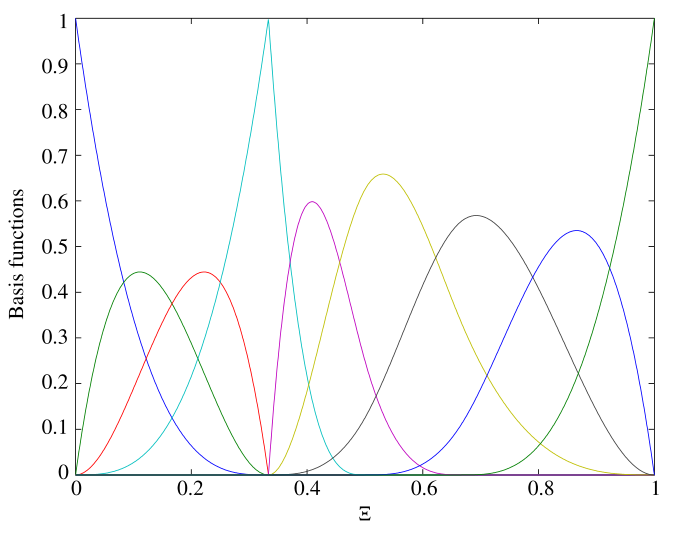
\includegraphics{literature/images/lr_nurbs_rational_basis.png}
    }
    \caption{3rd NURBS for an open knot vector $\Xi$ = \{ -1, -1, -1, -1, -1/3, -1/3, -1/3, 0, 1/3, 1, 1, 1, 1 \}. Note that the functions are only interpolatory at the end points}
    \label{lr_fig:nurbs_rational_basis}
\end{figure}

The first derivative of a NURBS basis function is computed using the quotient rule and is given by:
\begin{equation}
    \frac{d}{d\eta}R_{i,p}(\eta) =  w_i\frac{
        N^\prime_{i,p}(\eta)W(\eta) - N_{i,p}(\eta) W^\prime(\eta)
    }{W(\eta)^2}
\end{equation}

\section{Scaled boundary finite element method}
\label{lr_sec:sbfem}
\subsection{Scaled boundary finite element method in 2D elasticity}
\paragraph{}
The SBFEM is reviewed briefly in this section for two-dimensional elasticity.
Detailed derivation can be found in literature \cite{Wolf1996, WOLF20015551, Deeks2002}.
In the SBFEM, a scaling center O is selected at a point from which the whole boundary of the domain is visible (scaling requirement) (see Fig.~\ref{lr_fig:nurbs_rational_basis}).
The boundary of the domain can be represented with conventional finite elements as shown in Fig.~\ref{lr_fig:nurbs_rational_basis}.
The geometry of the domain has only to satisfy the scaling requirement.
This condition is automatically satisfied for all convex polygons and many concave polygons.
The scaling requirement is equivalent to the notion of `star convexity' \cite{Bishop2014}.
For the domain that does not meet the scaling requirement, the requirement can always be satisfied by sub-structuring, i.e. dividing the structure into smaller subdomains, for example, scaled boundary polygon formulation \cite{NATARAJAN2014101}.
\begin{figure}[!ht]
    \centering
    \scalebox{0.4}{
        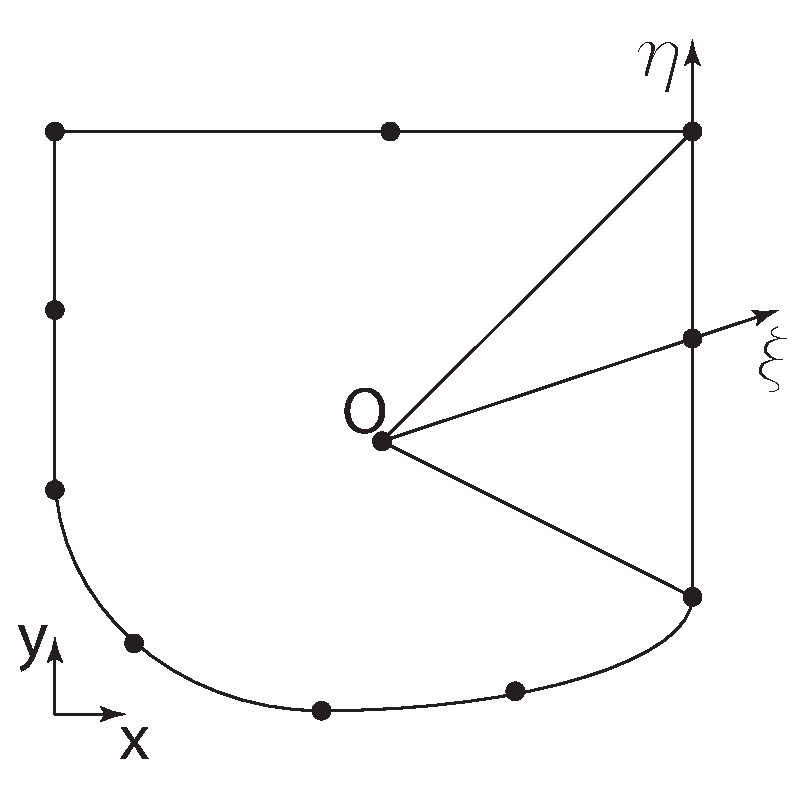
\includegraphics{literature/images/lr_sbfem_desc.eps}
    }
    \label{lr_fig:sbfem_desc}
    \caption{Two dimensional scaled boundary coordinates, where O is the scaling center and $\xi$ is the radial coordinate with $\xi=0$ at the scaling center and $\xi=1$ on the boundary.}
\end{figure}



\section{Adaptive mesh refinement}
% !TeX root = ../thesis.tex
\paragraph{}
In some situations, the FEM mesh can be so locally coarse that some localized phenomena can not be captured.
However, a naive implemented mesh generation algorithm usually produce a uniform mesh where small elements are created even though they are only necessary in limited areas.
X-FEM \citep{Moes1999} or the Generalized FEM \citep{STROUBOULIS20014081,doi:10.1002/nme.4954} was proposed to enrich the model when the mesh is so coarse that the local scale phenomena (crack for example) can not be taken into account.
Others developed the multigrid algorithms which permits relevant computations while keeping the computational cost acceptable to solve this problem \citep{doi:10.1002/nme.2427, doi:10.1002/nme.3037}.
However, only ad-hoc softwares support enriched finite element model or multigrid \citep{Duval2018}, which leads to the fact that these methods may not be applicable to all circumstances, especially for the users of the softwares that lack of such features.

\paragraph{}
As a consequence, methods using a posteriori error estimator to refine the mesh adaptively was proposed and widely adopted in FEM \citep{Duval2018, doi:10.1002/gamm.201490020,PRUDHOMME20091887,BAUMAN2009799, doi:10.1002/nme.1620121010, doi:10.1002/nme.1620240618,Oden1989,doi:10.1002/nme.1620240206,doi:10.1002/nme.1620330702,doi:10.1002/nme.1620330703, BOROOMAND1999127, ZIENKIEWICZ1999111, Ainsworth1993} and BEM \citep{Zhao1998, Guiggiani1990, KAMIYA1992223, KITA199421,ZHAO1999793,KITA2000317}.
A posteriori error estimator using stress recovery technique for the SBFEM was also proposed \citep{NME:NME439}.
However, some of these error estimators require extra work such as stress recovery.
Besides, it could be difficult to determine the most suitable error indicator to a given problem.
Machine learning and deep neural network introduced in Sec.~\ref{lr_sec:machine_learning} allows the usage of multiple error indicators was proposed \citep{SaeedIqbal;Graham.F.Carey2005}.
However, the fact that only the geometric properties were considered and the lack of physical indicators limit the effectiveness of this method.

\section{Machine learning}
\paragraph{}
A machine learning algorithm is such an algorithm that is able to learn from data and find regularities.
The ``learning'' is defined as ``A computer program is said to learn from Experience E with respect to some class of tasks T and performance measure P, if its performance at tasks in T, as measured by P, improves with experience E.'' \cite{Mitchell:1997:ML:541177}
\paragraph{}
The tasks T refer to the task that are too hard to solve with fixed programs.
For example, if a robot is designed to be able to walk, it can be done by a program that help the robot learn how to walk or by a program written manually to tell the robot how to walk.
The second option is rarely chosen because a fixed programs can hardly adapt the complex situation in the reality.
The tasks usually includes classification and regression problems in numerical calculation.
% The task in adaptive analysis will be classification.
% In this type of task, the algorithm is required to specify which category some input belongs to.
% Solving this task is to find a function $f: \mathbb{R}^n \rightarrow \{0,1\}$ where $0$ stands for ``not refine'' and $1$ for ``refine''.
% Each variable in the vector of the input $\pmb{x}$ in the function $y=f(\pmb{x})$ is a feature.

\paragraph{}
As a way to measure the abilities of a machine learning program, quantitative measurement of its performance must be designed.
Accuracy could be one of the most popular performance measurement in classification task.
It is simply defined as the rate of examples for which the algorithms gives the same classification as the reality.
In real world problem, the ability that a model performs on data that it has not seen before is more important as it is related to its performance when used in real world problem.
Consequently, these performance measures are usually evaluated using a subset of the original data called test set.
While another subset of the original data called training set are adopted to train the machine learning system.

\paragraph{}
A learning algorithm normally is either unsupervised learning or supervised learning.
It is depends on what kind of experience it has during the learning process.
Unsupervised learning algorithms experience a dataset that have a series of features.
It is expected to learn useful properties of this dataset.
While supervised learning algorithms experience a dataset that not only have many features, but also have a label or target.
For example, in Iris Fisher data set \cite{Fisher1936}, fish species of each iris plant will be included as well as features of the fish. 

\paragraph{}
Several supervised machine learning algorithms targeting classification problems will be introduced later.

% ------------------------------------------------------------------------------------ %
\subsection{Multilayer perceptron(MLP)}
\paragraph{}
There are plenty of machine learning algorithms such as Support Vector Machine (SVM)\cite{Boser1996,Cortes1995}, decision tree\cite{Olshen1984} and random forest\cite{Ho1995} that can be adopted in all kinds of situation.
Multilayer Perceptron(MLP), also known as feedforward neural networks or deep feedforward networks will be introduced in detail in this section as it is the method adopted in Chapter 5.

\paragraph{}
Fig.~\ref{lr_fig:ml_mlp_intro} illustrates an typical multilayer perceptron.
The reason why it is called feedforward is because that all calculation are conducted all the way from the inputs $x$ to the outputs $y$, passing the intermediate computations.
There is no feedback from a deeper layer to a shallower layer otherwise it becomes a recurrent neural network.
It is called neural networks is because that they are usually defined by a composition of several distinct functions.
These function can be described as an acyclic graph.
Take a function $f(x) = f^{(3)}(f^{(2)}(f^{(1)}(x)))$ as an example, it describe a MLP with three layers.
In this example, $x$ will be the input and the function $f^{(1)}$ is the first layer, $f^{(2)}$ being the second and the $f^{(3)}$ is called output layer.
Number of the functions or the length of the chains is called the depth of the neural network.
When a neural network with large number of layers, it is consider as a deep neural network and it is where the term ``deep learning'' comes from.
The training purpose of a MLP is to predict the output $y_p$ that is close to the accurate value $y_a$ from any given input $x_p$.
A training set with both inputs $x_t$ and expected outputs $y_t$ specify directly the behavior of the output layer upon different inputs.
There is no direct relationship between what other layers do and the training data.
A suitable learning algorithm is expected to be able to train these intermediate layers to response properly so that the prediction from the output layers is accurate enough.
These intermediate layers are called hidden layers as they are not directly related to the desired outputs.
\paragraph{}
Furthermore, the word neural illustrates that the idea of the topological model comes from neuroscience.
In the mathematical model of the neural network, each unit in a layer act independently like a neuron in human being's brain.
Even though a layer of these `neurons' forms a vector, the model can be more suitably described by each layer contains some neuron that behave analogously (dot production between two vectors) instead of a layer to layer relationship (matrix production between a vector and a matrix).
The choice of selecting more than one layers of vector and each neuron takes all values from the previous layer and then computed its own value to describe the model comes from the neuroscience while the functions used in the model is not guided by the neuroscience but by mathematical and engineering technologies.
A neural network so far will never aim to simulate a brain perfectly as well, it is designed to achieve statistical generalization instead.

\begin{figure}[!ht]
    \centering
    \scalebox{0.3}{
        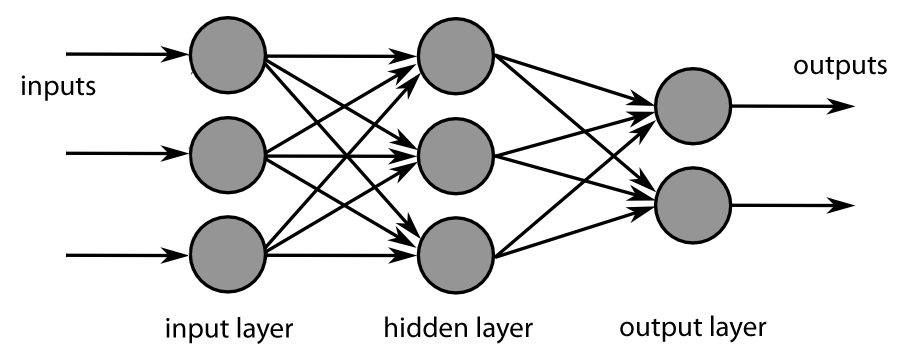
\includegraphics{literature/images/mlp_intro.png}
    }
    \caption{A typical topology of a multilayer preceptron}
    \label{lr_fig:ml_mlp_intro}
\end{figure}

\paragraph{}
The key question of a MLP is how to find a proper non-linear mapping function $\phi_i$ that can calculate all units in $i+1$-th layer from the previous one.
One of the options is to adopt a generic function, such as the Radial Basis Function(RBF)\cite{chang2010} kernel.
Even though an RBF kernel is capable to fit the training data with infinite-dimensional function, the performance on the test set usually not as satisfactory as it is on the training set.
Some advanced example can not be solved as not enough prior information is encoded and generic feature mappings drawn from the local smoothness is used only.
Another widely-accepted approach before the concept of deep learning being popular is to set the function manually.
Each used function for separated task typically spends engineers decades of time and it is very unlikely that these function can be used in other fields.
The strategy of deep learning is to find the function by itself based on the given training set.
In this approach, we have a model $y=f(x;\theta,\omega)=\phi(x;\theta)^T\omega$.
Where $\theta$ stands for parameters used to learn function $\phi$ from a large variety of functions.
Parameters $\omega$ then map the intermediate result $\phi(x)$ to the desired output.
Drawback of this method is that the convexity will not be guaranteed during the searching of the global minimum which means finding a local minimum based on gradient no longer means a global minimum.
However, the merits outweigh the shortcomings since the generalization is as high as using an RBF kernel and no human efforts is required.

\subsection{Gradient based optimization}
\paragraph{}
The learning problem of the MLP can be generalized as a optimization problem in mathematics.
In other words, the learning algorithm is to find the global minimum value of a specific value on a high dimensional surface.
The function need to minimize is called the criterion and it is called cost function or loss function when it is being minimized.
Fig.~\ref{lr_fig:ml_gradient_optimization} illustrates how the derivatives are used to perform a gradient descent algorithm on a parabola.
\begin{figure}
    \centering
    \scalebox{0.5}{
        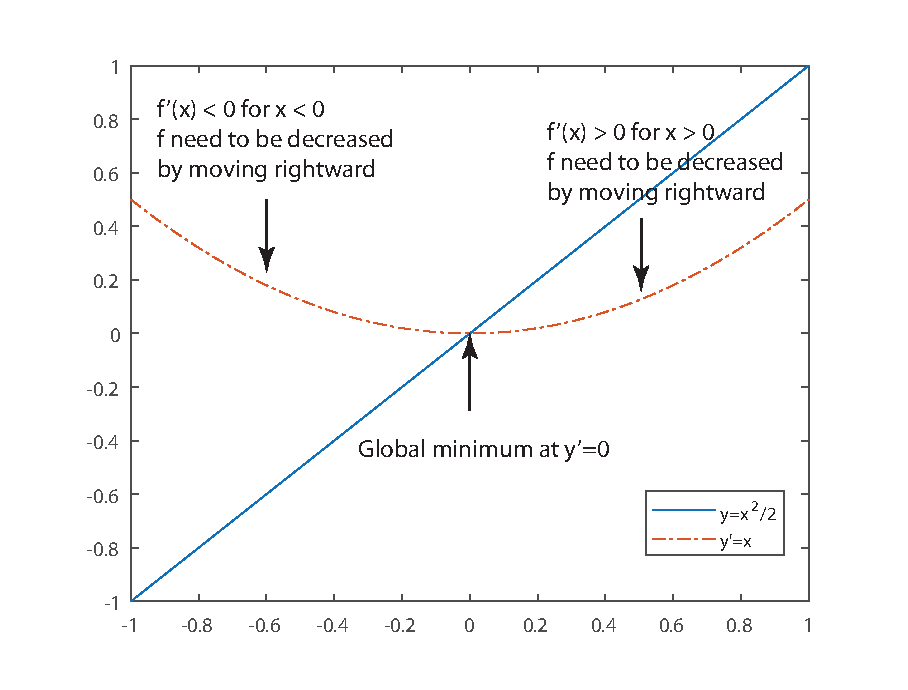
\includegraphics{literature/images/gradient_optimization.eps}
    }
    \caption{An example of gradient descent algorithm on a parabola}
    \label{lr_fig:ml_gradient_optimization}
\end{figure}

In a two dimensional curve who can be expressed by function $y=f(x)$ with real numbers $x$ and $y$.
The derivative $f^\prime=\frac{dy}{dx}$ is ultra useful to determine the global minimal value of a function as it stands for the slope and the slope tells whether $y$ is becoming smaller or larger when $x$ increase.
The global minimal is proved to happen when the derivative equal to zeros or on the boundary if the function is continuous.
While a point with zero slope does not necessary stands for a global minimal as it can be a local one or a saddle point.
\paragraph{}
In training problem of the MLP, chances are that we are end up with a multidimensional function that is not convex which creates extra challenge to determine the global minimal from local ones and saddle points surrounded by very flat regions.
As a consequence, in practice, the algorithm will be terminated when a small enough local minimal is found instead of looking for the global one.
In the situation where multiple input is involved, the concept of partial derivatives $\frac{\partial}{\partial x_i}f(x)$ is used to demonstrate the change in $y$ corresponding to the change in the $i$-th input $x_i$.
The gradient $\nabla_x f(x)$ contains the partial derivatives in all directions and hence are used in solving the learning problem in MLP.
In order to minimize loss function $f$, it is expected to determine the direction where $f$ decrease the fastest and it can be expressed in mathematical as
\begin{equation}
    \begin{aligned}
    & \argmin_{\mathbf{u}} \mathbf{u}^T \nabla_x f(x)\\
    = & \argmin_{\mathbf{u}} || \mathbf{u} ||_2 ||\nabla_xf(x)||_2 \cos\theta \\
    = & \argmin_{\mathbf{u}} \cos\theta
    \end{aligned}
\end{equation}
where $\mathbf{u}$ is a directional unit vector ($\mathbf{u}^T\mathbf{u}=1$) and $\theta$ is the angle between $\mathbf{u}$ and the gradient.
it can be concluded that $f$ can be decrease in the fastest way in the direction of the reverse of the gradient which is called gradient descent in Eq.~\ref{lr_eq:ml_gradient_descent}.
\begin{equation}
    x^\prime = x - \epsilon \nabla_x f(x)
    \label{lr_eq:ml_gradient_descent}
\end{equation}
where $\epsilon > 0$ stands for the learning rate which decided the distance for each step.
Several strategy exists to determine learning rate including using a tiny constant, adopting a large number at the beginning and decrease it during the iteration and try different learning rates and find the best (line search).

\subsection{Stochastic gradient descent (SGD)}
SGD is an extension of the gradient descent method described above in order to significantly decrease the computational time without lose the accuracy.
One commonly accepted way to improve the effectiveness of a MLP model is to increase the training set.
However, an increasingly large training set require more computational costs.
The cost function of a neural network can be written as followed when negative log-likelihood is used
\begin{equation}
    \mathbf{J}(\theta) = E_{\mathbf{x},y\sim\hat{p}_{data}}\mathbf{L}(\mathbf{x},y,\theta)
    =\frac{1}{m}\sum^m_{i=1}L(\mathbf{x}^{i},y^{i},\theta)
\end{equation}
where $L$ is the per-example loss $\mathbf{L}(\mathbf{x},y,\theta)=-log p(y|\mathbf{x},\theta)$.
And the calculation of the gradient descent becomes:
\begin{equation}
    \nabla_{\theta} \mathbf{J}(\theta)
    =\frac{1}{m}\sum^m_{i=1}\nabla_\theta \mathbf{L} (\mathbf{x},y,\theta)
\end{equation}
It is clear that the computation of the gradient is an $O(m)$ operation where $m$ is the size of the training data.
Considering the fact that it takes at least thousands iteration before a model converge and each iteration require an operation that takes prohibitively long time, some optimization must be taken.
The main idea of the SGD is to treat the gradient as an expectation.
Based on this assumption, the gradient can be calculated by some sampled data from the training set called minibatch $\mathbf{B}=\{x^{1},x^{2},\dots,x^{m^\prime}\}$ drawn from the original set.
Size of the minibatch $m^\prime$ is usually taken as an constant from one to a hundred and is irrelevant to the size of the training set unless the its size is extremely small (i.e. smaller than 100).
The gradient then can be calculated based on minibatch with $O(1)$ operation as
\begin{equation}
    g
    =\frac{1}{m^\prime} \sum^{m^\prime}_{i=1} \mathbf{L} (\mathbf{x},y,\theta)
\end{equation}

\paragraph{}
The most outstanding feature of the MLP compared to linear models is that it can capture non-linear features automatically which also result in a non-convex loss function.
As a consequence, learning algorithm in MLP adopt SGD to solve the optimization problem iteratively, instead of finding it directly with a closed form mathematical solution or by convex optimization.
This usually leads to a cost function with very low value rather than the global minimum.
Furthermore, without a convergence guarantee as non-convex loss function is treated and SGD is adopted, the selection of the initial value may have significant influence on the final result.
Hence, it is recommended to initialize all weights and bias to small values.

\subsection{Cost function}
\paragraph{}
Choosing a suitable cost function can be import to train a MLP.
In most of the case, maximum likelihood or negative log-likelihood performs reasonably satisfactory as the cross-entropy between the training data and the labels remains as for linear models.
It can be expressed as followed:
\begin{equation}
    \mathbf{J}(\theta) = -\mathbf{E}_{x,y\sim \hat{p}_{data}}  log   p_{model} (y|x)
    \label{lr_eq:ml_MLE}
\end{equation}
One of the outstanding merits to adopt this method is that the design of cost function for other model is no longer necessary.
Setting parameter for a model $p(x|y)$ and the cost function $log p(y|x)$ can be determined automatically.
Another advantage using maximum likelihood function as cost function is because that it helps to prevent gradient vanishing.
The gradient descent plays an important role in the learning algorithm and the method becomes inefficiency or even fail when the cost function becomes extremely flat (very small gradient).
In negative log-likelihood cost function, this kind of circumstance can be prevented because a logarithmic function saturate when the argument is extremely large.

\subsection{Output units}
\paragraph{}
The selection of the output units is highly related to the choice of the loss function.
In most of the case the cross-entropy between the distribution of the data and the model is used.
In other words, the form of the cross-entropy function decides the presentation of the output.
Although all output units can also act as a hidden unit, the major difference is that the output units must produce the result as expected.
\paragraph{}
In tasks where binary classification is expected, the sigmoid units is usually adopted.
The probability distribution of a binary classification is a Bernoulli distribution and the maximum-likelihood method is to define this distribution over $y$ conditioned on $x$.
The output of the neural net is to predict the probability $P(y=1|x)$ only as it is a binary classification.
By enforcing a constrain of $[0,1]$ on the probability, it becomes
\begin{equation}
    P(y=1|x) = max{0,min{1, w^T h + b}}
\end{equation}
assuming linear unit is adopted.
Even though a valid probability is defined, there will be some issue during the training as the gradient becomes zero when $w^T h +b>1$.
In gradient based learning algorithm, a zero gradient always cause problem because the algorithm may have very little information on how to improve the parameters.
In order to guarantee a non-zero gradient, a sigmoid output (Eq.~\ref{lr_eq:ml_sigmoid}) unit can be taken.
\begin{equation}
    \hat{y} = \sigma (w^T h +b)
    \label{lr_eq:ml_sigmoid}
\end{equation}
where $\sigma$ is the logistic sigmoid function
\begin{equation}
    \sigma = \frac{1}{1+e^{-x}}
\end{equation}

\paragraph{}
A sigmoid unit can be regarded as a combination of linear unit and a sigmoid activation function that convert the output from the linear component $z$ into a probability.
%-- need refactor
We omit the dependence on x for the moment to discuss how to define a probability distribution over y using the value $z$.
The sigmoid can be motivated by constructing an unnormalized probability distribution $\tilde{P}(y)$, which does not sum to 1.
We can then divide by an appropriate constant to obtain a valid probability distribution.
If we begin with the assumption that the unnormalized log probabilities are linear in $y$ and $z$ , we can exponentiate to obtain the unnormalized probabilities.
We then normalize to see that this yields a Bernoulli distribution controlled by a sigmoidal transformation of $z$:
%-- need refactor
\begin{equation}
    \begin{aligned}
        log \tilde{P} (y) &= yz \\
        \tilde{P} (y) &= e^{yz} \\
        P(y) &= \frac{e^{yz}}{\sum_{y^\prime=0}^1 e^{y^\prime z}} \\
        P(y) = \sigma ((2y-1)z)
    \end{aligned}
\end{equation}
Variable $z$ that define a distribution with normalization and exponentiation over binary variables is called logit

\begin{equation}
    \begin{aligned}
        J(\theta) &= -logP(y|x) \\
        & = -log \sigma ((2y-1)z) \\
        & = \zeta ((1-2y)z)
    \end{aligned}
\end{equation}
where $\zeta(x)$ is the softplus function 
\begin{equation}
    \zeta(x) = log(1+e^x)
\end{equation}

\paragraph{}
By rewrite the cost function in terms of softplus, it can be seen that saturation happens only when $(1-2y)z$ approaches negative infinity.
In other words, it happens when $y=1$ and $z$ approaches positive infinity which means the prediction is correct, or when $y=0$ and $z$ approaches negative infinity which means the prediction is extremely wrong.
In the later case, the softplus function can be simplified as
\begin{equation}
    \zeta((1-2y)z) = \zeta(|z|)
\end{equation}
And its derivative becomes $sign(z)$, which means the softplus function will not have gradient vanishing problem in the later case.
It helps the gradient descent learning algorithms to function with stability.

\subsection{Hidden units}
The choice of the hidden units lack of definitive principles and is still an active area of research.
Nevertheless, the rectified linear units (RELU) usually act as a default option.
RELU uses an activation function that maps $g(z)$ to $max\{0,z\}$ as shown in Fig.~\ref{lr_fig:ml_relu}
\begin{figure}[!ht]
    \centering
    \scalebox{0.4}{
        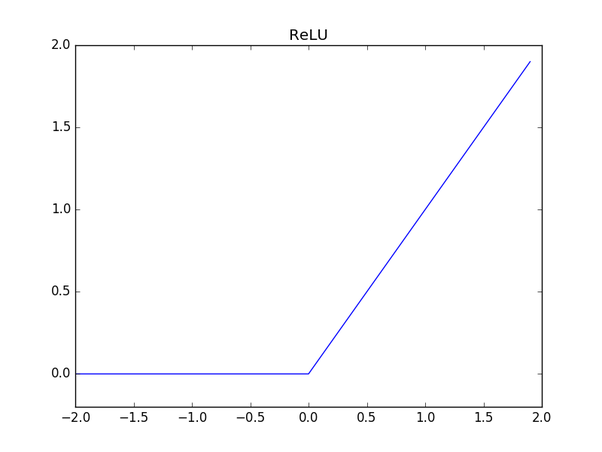
\includegraphics{literature/images/relu.png}
    }
    \caption{Rectified linear units}
    \label{lr_fig:ml_relu}
\end{figure}

\paragraph{}
Although it is not differentiable at $z=0$, the gradient descent still act as expected in practice.
This is because a numerical methods rarely find the local minimal, but end up with a point that is close enough to the local minimal.
Based on the assumption that a strict zero gradient is not expected, undefined derivatives can be allowed on hidden units.

\paragraph{}
One of the most outstanding advantage of the RELU is that it is extremely easy to optimize.
It is a linear unit expected for the fact that half of its domain yields zero.
As a consequence, the derivative of an RELU is significant if the unit is active.
RELU are applied on top of the existing affine transformation:
\begin{equation}
    \mathbf{h} = g( \mathbf{W}^T \mathbf{x} + \mathbf{b})
\end{equation}
Initial values for the transformation matrix are suggested to set with a small positive value as it can make most of the RELU active and let the derivatives pass through.
Because the output remain constant when it is inactive, the unit can not learn anything when it is not active.
Improvements has been proposed recently.
Absolute value rectification that map $g(z)$ to $|z|$ has been used in object recognition \cite{jarret2009}.
Leaky RELU that give a small positive value for the derivatives \cite{maas2013} while parametric RELU regard this derivatives as a learnable parameter \cite{He2015}.
Maxout units \cite{Goodfellow2013} is a further generalization of the RELU.
% --------- need refactor
instead of applying an element-wise function $g(z)$, maxout units divide $z$ into groups of $k$ values.
Each maxout unit then outputs the maximum element of one of these groups:
\begin{equation}
    g(z)_i = \max_{j\in G^{(i)}} z_j
\end{equation}
where $G^{(i)}$ is the set of indices into the input for group $i, \{(i-1)k+1, \dots, ik \}$.
This provides a way of learning a piecewise linear function that responds to multiple directions in the input $x$ space.
% ---------- need refactor
It can be regarded as learning the activation function as it actually learn a piecewise linear function.
High fidelity and any convex function can be achieved by maxout units if a large $k$ is used.
In practice, maxout units with $k=2$ usually have the same performance to traditional RELU, parametric RELU and Leaky RELU.
Since every maxout unit need to learn its own parameter, the size of the training set must be large enough to support the learning algorithms, or keep the $k$ value low \cite{Cai2013}.

\subsection{Architecture design}
\subsection{Back-propagation algorithm}




% ----------------------------------------------------------------- %

\subsection{Performance indicator}
\subsubsection{Confusion matrix}
A confusion matrix is a matrix used to illustrate the outcome of a classification model on a set of test data whose actual results are known.
    % Please add the following required packages to your document preamble:
    % \usepackage{multirow}
    \begin{table}[]
        \centering
        \caption{Confusion matrix}
        \label{my-label}
        \begin{tabular}{ccccc}
                                & & \multicolumn{2}{c}{\textbf{Predicted}}                 &  \\ \cline{3-4}
                                \multirow{3}{*}[-0.7em]{\textbf{Actual}} &
                                & \multicolumn{1}{|c|}{Refined}        & \multicolumn{1}{c|}{Not refined}    &  \\ \cline{2-4}        
                                & \multicolumn{1}{|c}{Refined}     & \multicolumn{1}{|c|}{True Positive(TP)}  & \multicolumn{1}{c|}{False Negative(FN)} &  \\ \cline{2-4}
                                & \multicolumn{1}{|c}{Not refined} & \multicolumn{1}{|c|}{False Positive(FP)} & \multicolumn{1}{c|}{True Negative(TN)}  &  \\ \cline{2-4}
        \end{tabular}
    \end{table}

\subsubsection{Accuracy}
\paragraph{}
Accuracy may be the most intuitive indicator.
It is simply defined as $\frac{TP+TN}{TP+TN+FP+FN}$
The importance of accuracy is dependent on the prior since the model can be highly influenced by the prior probability distribution.
For example, a spam detection model is trained from a data set which contains only 10\% of the spam e-mails.
As a consequence, if the model is extremely conservative and classify almost all incoming e-mails as non-spam, it can easily achieve an accuracy of more than 90\% in cross validation which is higher than lots of spam detectors.

\subsubsection{Precision(P)}
\paragraph{}
$$P=TP/(TP+FP)$$
Precision describes the chance that the model gives `true' and it is actually `true'.
In the spam detector example, a high precision can be expected as a conservative tends to give non-spam unless it has strong confidence.

\subsubsection{Recall rate(R)}
\paragraph{}
$$R=TP/(TP+FN)$$
Recall rate describes the ratio the model gives `true' to the total number of `true's.
In the spam detector example, a low recall rate is expected.

\subsubsection{F1 score}
\paragraph{}
$$F1 = 2*P*R/(P+R)$$
F1 score is an indicator that consider both the precision rate and the recall rate.
It is defined as the harmonic mean of them.

\subsubsection{Receiver operating characteristic(ROC)}
\paragraph{}
ROC is a True Positive Rate(TPR) vs False Positive Rate(FPR) curve (fig.~\ref{lr_fig:performance_roc}) where $TPR=R$ and $FPR=FP/(FP+TN)$
\begin{figure}[h!]
    \centering
    \scalebox{0.25}{
        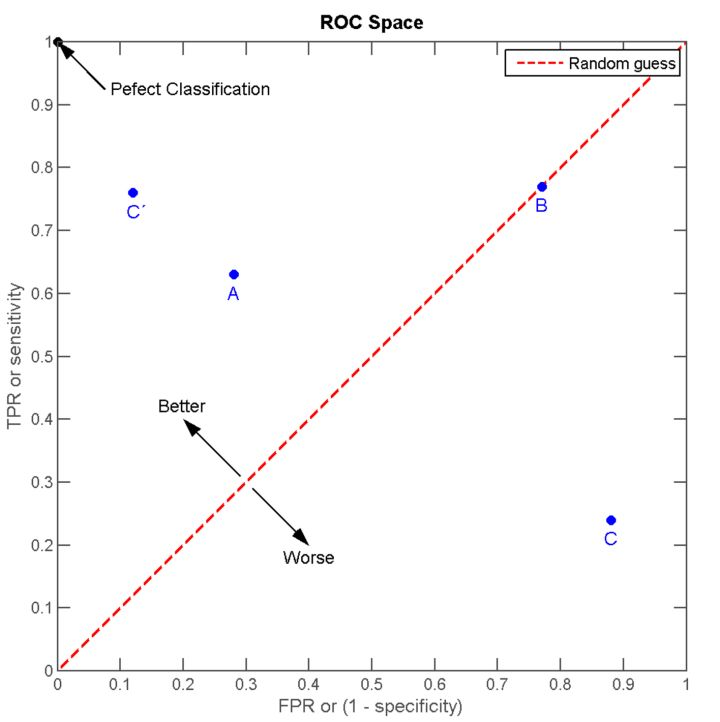
\includegraphics{adaptivity/images/svm_roc.jpg}
    }
    \caption{Receiver operating characteristic(ROC)}
    \label{lr_fig:performance_roc}
\end{figure}

\subsubsection{Area under the curve(AUC)}
\paragraph{}
As can be seen from ROC, the larger the area under the curve, the better the classifier is.
Consequently, area under the curve (AUC) becomes another important indicator in machine learning.

\section{Automatic mesh generation in 3D}
\paragraph{}
The FEM could be one of the most popular numerical method\hl{s} in engineering.
A necessary procedure is to discretize the problem domain into FE mesh of elementary shapes.
In 3D problem, the conventional FEM allows hexahedron, tetrahedron, wedge and pyramid only which limits the flexibility of mesh generation.
In order to achieve a reasonably accurate result, the mesh of the traditional FEM is required to conform to the boundary of the problem domain.
As a consequence, it could be necessary to develop an automatic mesh generation algorithm using limited types of shapes \citep{Frey:2007:MGA:1205626}.
The development of an automatic generation algorithm is reported to be able to save 80\% of the overall analysis time \citep{Hug2005}.

\paragraph{}
The research toward automatic mesh generation is popular over decades \citep{owen2000,Blacker1993,doi:10.1002/fld.1650081003,doi:10.1093/comjnl/24.2.167}.
Generally speaking, the hexahedral element is favored over the tetrahedral element in terms of accuracy but it could be difficult to generate the mesh with hexahedral elements only automatically.
Methods using plastering \citep{Blacker1993}, whisker weaving \citep{Tau1984}, sweeping \citep{Staten1999} and octree \citep{doi:10.1002/nme.1620201103} were proposed to generate a hexahedral mesh.
However, meshing of arbitrary domains using hexahedral element\hl{s} without losing the exact geometric representation is not achievable up to now.
Methods based on tetrahedral elements using Delaunay triangulation \citep{doi:10.1093/comjnl/24.2.167} and the advancing front technique (AFT) \citep{doi:10.1002/fld.1650081003} were proposed for arbitrary domains.
But Delaunay triangulation requires boundary recovery \citep{doi:10.1002/nme.808,LIU201432} and AFT need to solve colliding fronts \citep{Shewchuk1997}.
Furthermore, a mix use of all allowed elements \citep{owen2000} was proposed while the accuracy is not as satisfactory as that determined from the all-hexahedron mesh.

\paragraph{}
As a consequence, new numerical methods that reduce the limitation on element usage including X-FEM \citep{Moes1999}, isogeometric analysis \citep{Hug2005} (introduced in Sec.~\ref{lr_sec:iso_analysis}), finite cell method (FCM) \citep{Parvizian2007} and SBFEM \citep{Wol2003} (introduced in Sec.~\ref{lr_sec:sbfem}) were proposed.

\paragraph{}
The X-FEM eases the burden posed on mesh generation as conforming to the geometric boundary is not necessary.
Geometric discontinuity within the element is solved by the adoption of partition of unity \citep{MELENK1996289} and enrichment functions.
The method is then extended by the help of level-set \citep{OSHER198812} to be able to solve the holes \citep{Sukumar2001}, problems with material interfaces \citep{doi:10.1002/nme.2259} and flows \citep{Chessa2003}.
It has been applied in field of fluid-structure-contact interaction problems \citep{Mayer2010} and crack propagation for elastostatic problems \citep{doi:10.1002/nme.429,doi:10.1002/nme.430} in 3D.

\paragraph{}
In FCM, the mesh is generated by simple unfitted structured mesh of higher-order basis functions and the geometry is represented by averaging the adaptive quadrature points which removes the necessity of boundary conforming.
The method has been improved in terms of topology \citep{Parvizian2012} and applied to voxel model \citep{doi:10.1002/nme.3289} and problems with material interfaces \citep{Joulaian2013}.

\paragraph{}
Recently, an automatic mesh generation algorithm developed from the SBFEM and the octree-based algorithm using STL file (introduced in Sec.~\ref{lr_sec:stl}) was proposed \citep{Liu2017}.
Arbitrary element faces are allowed in the scaled boundary finite element which significantly decreases the limitation of element shape.
Mesh generated from an octree-based algorithm leads to higher quality elements and higher computational efficiency.
However, the geometry can not be retained exactly in the STL file which means the inevitable geometric imperfection may result in considerable accuracy issue \citep{Hug2005}.

 %
\subsection{STL file}
\label{lr_sec:stl}
\paragraph{}
STL file is another popular format which is used to represent the surfaces in CAD industry other than NURBS introduced in Sec.~\ref{lr_sec:NURBS}, especially in 3D printing and rapid prototyping \citep{Rengier2010,doi:10.1080/10426910902997571}.
One of the most promising advantages of the STL format is its simplicity.
Surfaces are divided into unstructured triangles but unexpected behaviors such as ill-shaped, overlapping and self-intersecting are allowed.
Although the STL can not represent the geometric information exactly, it has gained more popularity and wider application than that of NURBS.

\paragraph{}
As a result, several surface re-meshing methods \citep{BECHET20021,Wang2007227} were proposed in order to conduct the mesh generation from the STL files.
When used as the geometric input of the numerical method, a check of the unexpected behaviors including ill-shaped, overlapping and self-intersecting must be performed.
A mesh repairing \citep{Attene:2013:PMR:2431211.2431214} can be adopted when these behaviors are observed.
Furthermore, the elements generated will be in tetrahedral and the accuracy could be inferior to that determined from hexahedral elements even though high-quality triangular surface meshes is observed.


\section{Conclusions}
\paragraph{}
This chapter has summarized the linear theory of the Isogeometric analysis, together with a brief introduction on NURBS and its mathematical backgrounds, potentials and limitations.
A brief introduction on the IGES file is also presented.
Due to the dimensional mismatch, the SBFEM is the technique which can provide a seamless integration with the CAD modeling.
As a consequence, the SBFEM is enhanced with the idea of the Isogeometric Analysis, the automatic mesh generation and the adaptive mesh refinement.
The concept of the adaptive mesh refinement and its limitations are presented as well.
The MLP then is introduced to overcome this limitation by the adoption of multiple error indicators.
Finally, algorithm used to generate octree mesh in 3D from STL file is presented.
